% This is samplepaper.tex, a sample chapter demonstrating the
% LLNCS macro package for Springer Computer Science proceedings;
% Version 2.21 of 2022/01/12
%
\documentclass[runningheads]{llncs}
%
% T1 fonts will be used to generate the final print and online PDFs,
% so please use T1 fonts in your manuscript whenever possible.
% Other font encondings may result in incorrect characters.
%
% Used for displaying a sample figure. If possible, figure files should
% be included in EPS format.
%
% If you use the hyperref package, please uncomment the following two lines
% to display URLs in blue roman font according to Springer's eBook style:
%\usepackage{color}
%\renewcommand\UrlFont{\color{blue}\rmfamily}
%
%%%%%%%%%%%%%%%%%%%%%%%%%%%%SELF DEFINED AND INPUTS%%%%%%%%%%%%%%%%%%%%%%%%%%%%%%%%%%%%%%%%%%

\usepackage[T1]{fontenc}
\usepackage[normalem]{ulem}
\usepackage{mathtools}
\usepackage{blkarray,bigstrut} 
\usepackage{graphicx,wrapfig,lipsum}
\usepackage{tcolorbox}
\usepackage{enumitem}
\usepackage{array}
\usepackage{algorithm}
\usepackage{algorithmic}
\usepackage{mathpartir}
\usepackage{multirow}
\usepackage{hyperref}
\usepackage{amssymb}
\usepackage{subcaption}
\usepackage{stmaryrd}
\usepackage{color} 


\usepackage{tikz}
\usetikzlibrary{snakes}
\usetikzlibrary{svg.path} 
\usetikzlibrary{calc} 
\usetikzlibrary{shapes}
\usetikzlibrary{shapes.geometric}
\usetikzlibrary{arrows.meta}
\usetikzlibrary{arrows}
\usetikzlibrary{decorations.text,decorations.markings}
% % % % 

%%%%%%%%%%Packages for adaoption%%%

% \usepackage{amsthm} 

%Packages

\input{ldefs}
\newcommand{\highlight}[1]{\textcolor[rgb]{.0,0.0,1.0}{ #1}}
\newcommand{\THESYSTEM}{\textsf{PsRB}}

%%%%%%%%%%%%%%%%%%%%%%%%%%%%SELF DEFINED AND INPUTS%%%%%%%%%%%%%%%%%%%%%%%%%%%%%%%%%%%%%%%%%%

\begin{document}
%
\title{Path Sensitive Reachability Bound Analysis}
%
%\titlerunning{Abbreviated paper title}
% If the paper title is too long for the running head, you can set
% an abbreviated paper title here
%
%%%%%%%%%%%%%%%%%%%%%%%%%%%%Authors%%%%%%%%%%%%%%%%%%%%%%%%%%%%%%%%%%%%%%%%%%
% \author{First Author\inst{1}\orcidID{0000-1111-2222-3333} \and
% Second Author\inst{2,3}\orcidID{1111-2222-3333-4444} \and
% Third Author\inst{3}\orcidID{2222--3333-4444-5555}}
% %
% \authorrunning{F. Author et al.}
% % First names are abbreviated in the running head.
% % If there are more than two authors, 'et al.' is used.
% %
% \institute{Princeton University, Princeton NJ 08544, USA \and
% Springer Heidelberg, Tiergartenstr. 17, 69121 Heidelberg, Germany
% \email{lncs@springer.com}\\
% \url{http://www.springer.com/gp/computer-science/lncs} \and
% ABC Institute, Rupert-Karls-University Heidelberg, Heidelberg, Germany\\
% \email{\{abc,lncs\}@uni-heidelberg.de}}
%
%%%%%%%%%%%%%%%%%%%%%%%%%%%%Authors Above%%%%%%%%%%%%%%%%%%%%%%%%%%%%%%%%%%%%%%%%%%

\maketitle              

% typeset the header of the contribution
%
\begin{abstract}
    % The number of times a given control location 
    % inside a procedure is visited during the program execution.
    The upper bound on the number of times a given control location 
    inside a procedure is visited during program execution is referred to as the reachability-bound.
    %  by~\cite{GulwaniZ10} in the first place.
    % A tight reachability-bound
    % can help to improve the analysis result on other program features.
    % While computing a tight reachability-bound for a given program control location is challenging.
    % Many works in the program analysis area develop algorithms estimating the program's loop bound or overall complexity.
    % But there isn't a general analysis algorithm that
    % computes the reachability-bound
    % directly or path-sensitively.
    % To leverage these limitations,
    This paper presents a path-sensitive reachability-bound algorithm
    aiming to find a precise symbolic reachability-bound \todo{on the program's every control location path-sensitively}.
    %  in this paper.
    In comparison with previous methods, our algorithm brings together two lines of program complexity analysis techniques:
    1. amortized bound analysis through program abstraction and ranking function estimation, and
    2. loop summarization based multiple loop paths refinement.
    Built on the combination, we introduce two new quantities, \emph{path reachability-bound} and \emph{loop reachability-bound}.
    % combines them effectively. 
    This effective combination leverages the precision and efficiency trade-off between the two lines of techniques.
    It allows us to compute precise reachability-bound on each program point path-sensitively.
    We implement a prototype and report on an experimental comparison with state-of-art tools over four different benchmarks.
\keywords{Loop Bound Inference, program refinement, path-sensitive}
\end{abstract}
%
%
%

%%%%%%%%%%%%%%%%%%%%%%%%%%%%%%%%%%%%%%%%%%%%%%%%%%%%%%%%%%%%%%%%%%%%%%%%%%%%%%%%%%%%%%%%%%%%%%%%%%%%%%%%%%%%%%%%%%%%%%%%%%%%%%%%%%%%%%%%%
%%%%%%%%%%%%%%%%%%%%%%%%%%%%%%%%%%%%%%%%%%%%%%%% The Introduction and Overview %%%%%%%%%%%%%%%%%%%%%%%%%%%%%%%%%%%%%%%%%%%%%%%%%%%%%%%%
%%%%%%%%%%%%%%%%%%%%%%%%%%%%%%%%%%%%%%%%%%%%%%%%%%%%%%%%%%%%%%%%%%%%%%%%%%%%%%%%%%%%%%%%%%%%%%%%%%%%%%%%%%%%%%%%%%%%%%%%%%%%%%%%%%%%%%%%%
\section{Introduction}
\label{sec:intro}

Gulwani et. al~\cite{GulwaniZ10} first introduce \emph{reachability-bound} as the upper bound on the number of times a given control location 
inside a procedure is visited during program execution.
A tight reachability-bound has many applications.
For example from a privacy and security perspective,
how much secret information is leaked by a program depends on the number of times a certain operation that leaks the data
is executed~\cite{Malacaria07};
from an efficiency perspective, when different program locations consume different resources, a precise reachability-bound of each location can help to estimate the resource cost more accurate than just computing the overall complexity.
While existing works all have different limitations when inferring the \emph{reachability-bound}.
For example, Gulwani et. al~\cite{GulwaniZ10}
give a two-step solution by combining program abstract and proof-rules-based bound computation.
But it does not compute the \emph{reachability-bound} precisely for every control location.
Instead, they only compute the complexity bounds for overall loop and over-approximate for different locations using this bound,
which is loose especially when there are multipath loops.
Techniques in program complexity analysis~\cite{GustafssonEL05,HumenbergerJK18} 
or worst-case resource cost analysis
~\cite{BrockschmidtEFFG16,AlbertAGP08,AliasDFG10,Flores-MontoyaH14} can be repurposed to estimate similar quantities such as the
bounds on loop iterations, execution time, etc.
While these quantities focus only on  
the overall complexity,
none of them compute the reachability-bound on a given program control location directly or path-sensitively.
This leads to inaccuracy in data leakage analysis, resource cost estimation, etc.
To overcome these limitations, 
we introduce a novel path-sensitive reachability-bound analysis algorithm that solve 
the reachability-bounds problem efficiently and path-sensitively.
It is built over an abstract transition graph which effectively combines amortized complexity analysis with loop summarization based multipath refinement.
This combination mitigates the limitations faced by either technique individually. 
Before diving into the algorithm, below are some related works and their limitations.

% \begin{itemize}
% \item 
\emph{Program Abstraction.}
Program abstraction is commonly used in program analysis as a preprocessing step to abstract program features and generate transition graphs or systems. For example, Gulwani et. al~\cite{GulwaniZ10} summarizes programs into some underlying abstract domains (the unified lattice~\cite{CousotH78}, polyhedra~\cite{CousotC77} or octagonal~\cite{Mine06})
and generates transition systems for loop counters.
\cite{KincaidCBR18} abstracts program into the wedge domain and computes the non-linear loop invariant.
%  While it only works well for the specific targeting problem.
Efficiency is the main bottleneck when generating and solving the constraint.
We choose to use the difference constraint based program abstraction model~\cite{SinnZV17,SinnZV14} combined with boolean expression to generate our abstract transition graph.
It is more accurate in the sense of representing the program loops path-sensitively. This representation is also comparatively lightweight.

% \item 
\emph{Amortized Complexity Analysis.}
One line of complexity analysis follows the idea of the \emph{amortized complexity analysis}
originated from Tarjan's influential paper~\cite{PotechinP17}. It is usually combined with ranking functions~\cite{BradleyMS05,CookSZ13,Zuleger18} or counter increments~\cite{ZulegerGSV11,SinnZV14,SinnZV17,LuCT21,AliasDFG10}.
They do well in nested loops by alternating the loop bound computation with the ranking or counter estimation. This alternation is efficient without recursively unrolling the nested loops when composing the bound of different paths.
  % \\
  But estimating the counter or ranking function invariant ignores the interleaving between multiple paths in the same loop,
% Most of them 
such as the tools CofloCo~\cite{Montoya17,Flores-MontoyaH14,Flores-Montoya16}, KoAT~\cite{BrockschmidtEFFG16,BrockschmidtEFFG14,FalkeKS12,FalkeKS11}, the algorithm in~\cite{LuCT21}, and etc.
%  over-approximate the loop bound when the path interleaving affects loop execution.
It is hard to repurpose their result as the reachability-bound on different points.
% loop bound path-insensitively as the reachability-bound on different points.
Another kind of \emph{amortized complexity analysis} based on type refinement or annotation~\cite{CraryW00,JostHLH10,CicekBG0H17,RajaniG0021,CarbonneauxHS15} has the same weakness in the multipath loops, resulting in the over-approximation of the resource cost on different program points.
To overcome these limitations, we enrich it with path-sensitivity according to the Alg.~2 in~\cite{SinnZV14},
% which assigns a variable to each edge on which this variable decrease as its ranking function.
the Alg.~3 in~\cite{ZulegerGSV11},
and the Def.~25 in Section 4 from~\cite{SinnZV17}.

\emph{Loop Summarization and Path Refinement Based Complexity Analysis}.
Another line of loop bound analysis through loop summarization and path refinement seeks for precise loop path representation~\cite{ManoliosV06,BalakrishnanSIG09,SharmaDDA11,Flores-MontoyaH14,HumenbergerJK18,CyphertBKR19}, and explicating the interleaving between paths~\cite{GulwaniJK09,ZulegerGSV11}.
\cite{KincaidBCR19,KincaidCBR18,BreckCKR20} introduce some loop summarization techniques which can help to improve the accuracy of the path refinement but specifically for non-linear loops, program recurrence, etc.
%  summarization techniques~\cite{KincaidCBR18} and the invariant generating algorithm considering recurrence in~\cite{BreckCKR20}. 
However, when composing the bound between nested loops, recursively unrolling the nested loops is heavy and non-terminating in most cases.
%
Our method simplifies the path refinement algorithm in~\cite{GulwaniJK09} using contextualization techniques based on~\cite{ZulegerGSV11,SinnZV14,ManoliosV06}.
We also limit the iterations of the refinement algorithm to a constant in our bound analysis algorithm.
% \end{itemize}
%

We perform both path refinement and ranking estimation over an abstract transition graph through program abstraction presented in Section~\ref{sec:progabs}.
This combination utilizes the effectiveness of \emph{amortized complexity analysis} by computing the ranking function
% $\locbound(\absevent, c)$ for each transition edge $\absevent$, 
and estimating its bound invariant in Section~\ref{sec:rank}.
It additionally benefits from the accuracy of path refinement techniques through a light-weight path refinement algorithm adopted from~\cite{GulwaniJK09} in Section~\ref{sec:refine}.
Building on this combination, we introduce two novel quantities,
the \emph{path reachability-bound} and \emph{loop reachability-bound}.
The first one bounds the evaluation times of each loop free and interleaving free path in a refined program, and the second one bounds the iterations of an outer loop w.r.t. the innermost loop such that in these iterations of outer loop, the innermost loop is ``entered''. 
Then we present the algorithm for estimating the two quantities in Section~\ref{sec:looprb} and~\ref{sec:pathrb} and compute the \emph{reachability-bound} for each program point path-sensitively in Section~\ref{sec:psrb}.
Our evaluation on the prototype implementation in Section~\ref{sec:eval} shows that we can accurately estimate different bounds for different program points on multiple loop paths. By summing up the different \emph{reachability-bound}s on every location, the results shows a big improvement comparing to the state-of-art worst case complexity analysis.

To recapitulate, our main contributions are summarized as follows.
\\
% \begin{itemize}
%   \item 
1. A path-sensitive reachability-bound algorithm which computes sound bound on the evaluation times of each program point path-sensitively.
\\
%  \item 
2. The combination of \emph{amortized bound analysis} through ranking function estimation and the path refinement approach in our algorithm.
% \item 
\\
3. Two novel quantities, the \emph{path reachability-bound} and \emph{loop reachability-bound} and their corresponding estimating algorithms.
% \item 
\\
4. A prototype implementation with evaluation over four different benchmarks.
  The evaluation shows big improvement comparing to the state-of-art worst case complexity analysis, and potential applications in other areas.
% \end{itemize}
% %


\section{Technique Challenges and Algorithm Overview}
\label{sec:overview}
In this section, we discuss a representative running examples with
challenges of analyzing the symbolic
\emph{reachability-bound} on
every control location and illustrate our key novelties, \emph{path reachability-bound} and the \emph{loop reachability-bound}.
This example is adopted from the example in~\cite{GulwaniZ10}, which
is a skeleton code from the .Net base-class library.

% \paragraph{Challenges.}
\begin{example}
  [The Running Example with Two Paths Loop and Nested Loop in One Path]
  \label{ex:relatedNestedWhileOdd_abscfg}
    { \small
  \begin{figure}
  \centering
  \begin{subfigure}{.4\textwidth}
    \begin{centering}
    {\small
    $
    \begin{array}{l}
      \kw{nestedOdd}(n, m) \triangleq \\
      \clabel{ \assign{i}{n} }^{0} ; \\
          \ewhile ~ \clabel{i > 0}^{1} ~ \edo ~ \\
          \qquad \Big(
            \eif(\clabel{i \% 2 \neq 0 }^{2},\\
            \qquad \clabel{\assign{k}{i - m}}^{3};\\
            \qquad \ewhile ~ \clabel{k > 0}^{4} ~ \edo ~
            \Big( \clabel{\assign{k}{k - 1}}^{5} \Big);\\
            \qquad \clabel{\assign{i}{k + m}}^{6};
            \clabel{\assign{i}{i - 1}}^{7}, \\
            \qquad \clabel{\assign{i}{i - 3}}^{8})
            \Big)
      \end{array}
    $
    }
    \caption{}
    \end{centering}
    \end{subfigure}
  \begin{subfigure}{.5\textwidth}
    \begin{centering}
  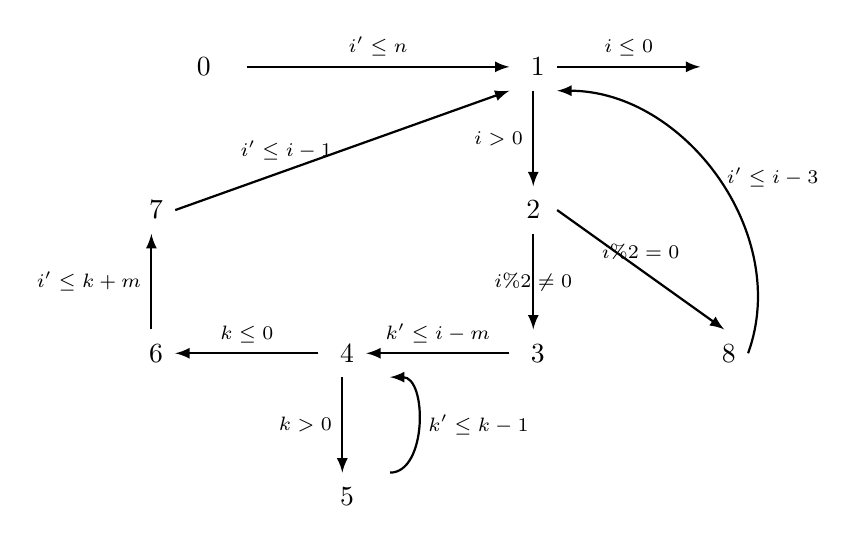
\begin{tikzpicture}[scale=\textwidth/20cm,samples=200]
  \draw[] (-7, 10) circle (0pt) node{{ $0$}};
  \draw[] (0, 10) circle (0pt) node{{ $1$}};
  \draw[] (0, 7) circle (0pt) node{\textbf{$2$}};
  \draw[] (0, 4) circle (0pt) node{{ $3$}};
  \draw[] (-4, 4) circle (0pt) node{{ $4$}};
  \draw[] (-8, 4) circle (0pt) node{{ $6$}};
  \draw[] (-4, 1) circle (0pt) node{{ $5$}};
  \draw[] (4, 4) circle (0pt) node{{ $8$}};
  \draw[] (-8, 7) circle (0pt) node{{ $7$}};
  % Counter Variables
  \draw[] (4.5, 10) circle (0pt) node {\textbf{$\lex$}};
  % \draw[] (6, 4) circle (0pt) node {{ $ex$}};
  %
  % Control Flow Edges:
  \draw[ thick, -latex] (-6, 10)    -- node [above] {\scriptsize $i' \leq n$}(-0.5, 10);
  \draw[ thick, -latex] (0, 9.5)    -- node [left] {\scriptsize $i > 0$} (0, 7.5) ;
  \draw[ thick, -latex] (0.5, 7)    -- node [above] {\scriptsize $ i \% 2 = 0 $}  (4, 4.5);
  \draw[ thick, -latex] (4.5, 4)    to  [out=70,in=0]   node [right] {\scriptsize $i' \leq i - 3$ }(0.5, 9.5);
  \draw[ thick, -latex]  (0, 6.5)   -- node  {\scriptsize $i \% 2 \neq 0$}  (0, 4.5) ;
  \draw[ thick, -latex]  (-0.5, 4)  -- node [above] {\scriptsize $k' \leq i - m$ }  (-3.5, 4) ;
  \draw[ thick, -latex]  (-4.5, 4)  -- node [above] {\scriptsize $k \leq 0$ }  (-7.5, 4);
  \draw[ thick, -latex] (0.5, 10)   -- node [above] {\scriptsize $i \leq 0$}  (3.5, 10);
  \draw[ thick, -latex] (-4, 3.5)   -- node [left] {\scriptsize $k > 0$}  (-4, 1.5);
  \draw[ thick, -latex] (-3, 1.5)   to  [out=0,in=0] node [right] {\scriptsize $k' \leq k- 1$}  (-3, 3.5);
  \draw[ thick, -latex] (-8, 4.5)   --  node [left] {\scriptsize $i' \leq k + m$ }(-8, 6.5);
  \draw[ thick, -latex] (-7.5, 7)  --  node [left] {\scriptsize $i' \leq i - 1$ }(-0.5, 9.5);
  % \draw[ thick, -latex] (6, 6.5)  -- node [right] {$\top$} (6, 4.5) ;
  \end{tikzpicture}
  \caption{}
    \end{centering}
    \end{subfigure}
\begin{subfigure}{.9\textwidth}    
\begin{centering}
  {\small
  $\tpath_0 = (0 \to 1)$
  \quad
  $\tpath_1 = (1 \to 2 \to 3 \to 4)$
  \quad
  $\tpath_2 = (4 \to 6 \to 7 \to 1)$
  \quad
  $\tpath_3 = (4 \to 5 \to 4)$
  \quad
  $\tpath_4 = (1 \to 2 \to 8 \to 1)$
  \quad
  $\tpath_5 = (1 \to \lex)$
  \\
  $
  \tpath_0 ; \rpchoose{ 1: \rprepeat(\tpath_1; 4:\rprepeat(\tpath_3); \tpath_2; \tpath_4), 
  1: \rprepeat(\tpath_4; \tpath_1; 4:\rprepeat(\tpath_3); \tpath_2) }; \tpath_5
  $
  }
  % \caption{}
    \end{centering}
    \end{subfigure}
  \caption{
  (a) The program of the two paths loop with a nested Loop in one path,
    (b) The corresponding \emph{Abstract Transition Graph}, $\absG(\kw{nestedOdd}(n, m))$. }
      \label{fig:relatedNestedWhileOdd-overview}
  \end{figure}
  }
  %
  \end{example}    
  
\footnotetext{We use the notation $(l_0 \to \cdots \to l_n)$ to denote a vertices sequence $(l_0, \cdots, l_n)$, and the constraint on each edge in each transition path are omitted for concise.}
% \todo{Shorten}
% \begin{itemize}
%   \item 
\textbf{Challenge I}
  In this example, given $n \geq m$,
the precise \emph{reachability-bound}s for control locations $4$ and $5$ are both $m \times \lfloor\frac{n}{m}\rfloor$,
for location $2$ and $3$ are $(m + 1) \times \lfloor\frac{n}{m}\rfloor + 1$, 
and $1$ for locations $0, 1$ and $\lex$. 
\highlight{Notice here, though within the same loop $L_2$, the bounds for locations $4$ and $5$ on the first branch, and $6$ on the second branch are different.}
\\
However, the state-of-art \emph{reachability-bound} analysis~\cite{GulwaniZ10}
gives the same \emph{reachability-bound}, $n + \lfloor\frac{n}{m}\rfloor$ for all the locations within the loop $L_2$, which is tight w.r.t. $L_2$'s iteration times but not for different locations inside $L_2$ without considering multiple paths.
Among works on program complexity, cost and loop bound analysis, \cite{GulwaniJK09} can also compute the tight bound on the loop iteration but not reachability-bound on each location path-sensitively.
Though we can use it as the \emph{reachability-bound} for location $1$ and $2$,
the \emph{reachability-bounds} for control locations $4, 5$ and $6$ are still unclear.

This motivates us the first key novelty -- the \emph{path reachability-bound} $\inoutB(\rprog, \tpath)$ for a loop free path $\tpath$ within a loop program $\rprog$ bounds the evaluation times of each loop free path instead of the entire multipath loop.
% \item 

\textbf{Challenge II}
  Then in line 8, $i$ is reset by $w$ and $w$ is reset by $j$ at line 5. So the
while $L_6$ is only executed in the first iteration of while loop $L_1$ and $L_3$.
% \\
The while loop $L_3$ at line 3 is executed only in 
the first $m - N$ iterations of the 
$L_1$ because $j$ is reset by $i$ in line 2.
% \\
So the total iterations of all the three loops is
$n + m^2 - m \times N$,
and the precise \emph{reachability-bound} for location $7$ inside the $L_6$ is $N$,
for locations $4, 5$ and $8$ between the $L_3$ and $L_6$ are $(n-N) \times (m - N)$,
and $n - N$ for locations $2$ and $9$.
% \\
\highlight{Notice here the \emph{reachability-bounds} for the locations inside the loop $L_6$ is 
the same as its innermost loop iteration bound.
% , as well as our \emph{path reachability-bound}.
However, for the locations between $L_3$ and $L_6$,
the \emph{reachability-bounds} are the multiplication of the inner and outer loop iteration bounds.}
\\
To the best of our knowledge, the loop bound analysis method in \cite{GulwaniJK09} can only give a loose bound $n + (m \times n) + N$ for the entire loop complexity, and 
the DC-based algorithm in \cite{SinnZV17} is able to
compute a better but still loose bound, $n + m^2 - m \times N$ on total iteration times.
None of them can give the precise \emph{reachability-bound} for every location in these nested loops,
which is non-trivial to compute even though knowing the loop bound.
% especially for the locations similar to $7$ in $\kw{threeNestedWhile}$.

\highlight{
This motivates use consider our second novel quantity --
the numbers of iterations of the outside loop $L_3$ and $L_1$ such that,
during these iterations, the loop $L_6$ is ``entered''. 
We call this the \emph{loop reachability} of the location within loop $L_6$ w.r.t the loops $L_3$ and $L_1$.
Then by multiplying the loop iteration bound of the $L_6$ with its \emph{loop reachability} times w.r.t the  $L_3$ and $L_1$, we can compute the precise
\emph{reachability-bounds} for location $7$.
}

\highlight{
This quantity isn't considered or computed in any of the previous works.
In the line of methods based on path refinement and loop summarization, the \emph{Progress Invariant} method in \cite{GulwaniJK09} is only able to compute
the
bound on iteration numbers
of the inner loop $L_6$ in each iteration of $L_3$ and $L_1$, which are both $N$.
So they have to over-approximate the reachability-bound for locations inside $L_6$ with the
overall program complexity by multiplication, i.e., $n + m^2 - m \times N$.
In the line of the \emph{amortized complexity analysis} through ranking function, the DC-based algorithm in \cite{SinnZV17}
is only able to
compute the combined loop bound and the local bound of each loop
separately as well.
% We are still unable to know the precise \emph{reachability-bound} for the locations in the innermost loop.
}
% \end{itemize}
With the two key novelties, our algorithm computes the reachability-bound for this example through the following steps.
% \paragraph{Main Steps of Path-sensitive Reachability-bound Analysis}
% \label{sec:static_rb}

\textbf{\emph{Step1: Program abstraction.}}
In Section~\ref{sec:progabs},
we first 
generate the \emph{Abstract Transition Graph} as in Figure~\ref{fig:relatedNestedWhileOdd-overview}(b).
Each edge $l \xrightarrow{dc} l'$ is an abstract transition $\absevent = (l, dc, l')$ annotated with a constraint $dc$ corresponding to the command of label $l$.

Then we abstract the program in the form of paths.
$$
\tpath_0 ; \rpchoose{ 1: \rprepeat(\tpath_1; 4:\rprepeat(\tpath_3); \tpath_2), 1:\rprepeat(\tpath_4) }; \tpath_5
$$
$;$ concatenates sequence of execution paths,
$\rprepeat(\tpath_3)$ represents looping on the path $\tpath_3$ and
$\rpchoose{ \ldots}$ represents the loop $L_1$ which contains two possible execution paths,
$\rprog_1 = \tpath_1; 4:\rprepeat(\tpath_3);\tpath_2$ and $\rprog_2 =\tpath_4$.

% \textbf{Step 2: Program Refinement}
\textbf{\emph{Step 2: Path interleaving refinement.}} 
Two execution paths are not simply iterating on themselves during the program execution,
they could interleave each other at certain iteration.
We summarize each execution path into conjunctions of transition relations.
\begin{equation}
    \begin{array}{l}
        \rprog_1 \models \phi_1 = \\
    \rprog_2 \models \phi_2 = 
    \end{array}
\end{equation}
  
In this sense, Algorithm~\ref{alg:prog-refine} in Section~\ref{sec:refine} computes the interleaving orders
by exhaustively checking the compositions of transition relations of different execution paths,
\begin{equation}
    \begin{array}{l}
        \rprog_1 ; \rprog_1 \models \exists i, k \st \phi_1 \circ \phi_1 = ... \implies \efalse\\
        \rprog_2 ; \rprog_2 \models \exists i, k \st \phi_2 \circ \phi_2 = ... \implies \efalse \\
        \rprog_2 ; \rprog_1 \models \exists i, k \st \phi_2 \circ \phi_1 = ...  \\
        \rprog_1 ; \rprog_2 \models \exists i, k \st \phi_1 \circ \phi_2 = ... 
    \end{array}
\end{equation}
Only two execution paths are feasible, so we identify two unique interleaving orders --
either $\rprog_1$ executes after one iteration of $\rprog_2$ or vice versa.
% Then, loop $L_1$ in the source program is generates new execution paths as follows,
\[
    \rprog^1 = \rprog_1 ; \rprog_2 = \tpath_1; 4:\rprepeat(\tpath_3); \tpath_2; \tpath_4
    \qquad
    \rprog^2 = \rprog_2 ; \rprog_1 = \tpath_4; \tpath_1; 4:\rprepeat(\tpath_3); \tpath_2
\]
% The second step in Section~\ref{sec:refine}
Then, the multiple-paths loop $L_1$ in the source program is refined
into multiple loops where each one can only iterate following the specified interleaving order.
% the interleaving of paths is explicit.
As in the bottom of Figure~\ref{fig:relatedNestedWhileOdd-overview}(c),
the program is transformed into 
\[
    \tpath_0 ; \rpchoose{ 1: \rprepeat(\tpath_1; 4:\rprepeat(\tpath_3); \tpath_2; \tpath_4), 
1: \rprepeat(\tpath_4; \tpath_1; 4:\rprepeat(\tpath_3); \tpath_2) }; \tpath_5
\]
In this refined program, 
each new execution path is equivalent to the execution of the original loop. 
% denoted as $\rprog_1^1$ and $\rprog_1^2$.

% \textbf{Step 3: Ranking Function Estimation}
\textbf{\emph{Step 3: ranking function estimation.}}
Algorithms in Section~\ref{sec:rank} identifies the ranking function for each transition edge, which is a symbol whose number of decreasing times can represent the number of execution of this edge.
For example for edge $4 \to 5$, its ranking function is $k$ and edges on $\tpath_1$, $\tpath_2$ and $\tpath_4$ all have $i$ as their ranking functions.

% \textbf{Step 4: Path-sensitive Reachability-bound Computation.}
\textbf{\emph{Step 4: local path reachability-bound.}}
For $\tpath_3$ in the program in Figure~\ref{fig:relatedNestedWhileOdd-overview}, we want to know how many times it is ``reached'' during the program execution.
From the refined program, $\tpath_3$ shows up in both newly generated execution paths $\rprog^1$ and $\rprog^2$  and nested in two level loops.
The algorithm in Section~\ref{sec:pathlocalrb} first
% computes a local \emph{path reachability-bound} for it w.r.t. its innermost loop $L_4$ by computing 
computes three abstract states for the ranking functions on $\tpath_3$ when first, second and last visiting during execution of $L_4$,
\begin{equation*}
    \rfinit(\rprog^1, \tpath_3, c) = \{k = n - m\} \quad
    \rfnext(\rprog^1, \tpath_3, c) = \{k = 1\} \quad
    \rffinal(\tpath_3, c) = \{ k = 0 \}.
\end{equation*}
Then  the maximal value of the following formula provides   
an upper bound on the number of execution times of $\tpath_3$ when executing only the innermost loop where $\tpath_3$ is nested. 
\[
    \max
    \left\{ 
        {\frac{a - b}{1}} 
        ~\vert~
        x = a \in \{k = n - m\}
        \land x = b \in \{ k = 0 \}
    \right\}  = n - m
\]
% The algorithm in Section~\ref{sec:pathlocalrb}
% computes $\outinB(4:\rprepeat(\tpath_3), \tpath_3, c) = n - m$ by computing
% the initial state, next state and final state of ranking functions on $\tpath_3$ during the execution of $\rprepeat(\tpath_3)$.

\textbf{\emph{Step 5: loop reachability-bound.}}
Previous step only provides the path reachability-bound for a simple transition path w.r.t. the innermost loop.
For nested loops, we need to compute the \emph{loop reachability-bound} for each simple transition path with respect to every level of the outer loop.
Since $\tpath_3$ is nested in two level loops, we compute its \emph{loop reachability-bound}
with respect to the outer loop $L_1$. 
It is expected to be $1$ because the inner loop $L_4$ is reached only in the first iteration of the outer loop $L_1$.
% , we aim to compute $1$ as the \emph{loop reachability-bound} of $\tpath_3$ w.r.t. $L_1$.
In the first refined execution path, $\rprog^1 = \rprepeat(\tpath_1; 4:\rprepeat(\tpath_3); \tpath_2; \tpath_4)$,
we compute three abstract states when visiting $L_4$ the first, second and last time during the execution of loop $\rprog^1$,
\begin{equation*}
\lpinit(\rprog^1, \tpath_3, c) = \max\{ n - m\} \quad
\lpnext(\rprog^1, \tpath_3, c) = \max\{n - m\} \quad
\rffinal(\tpath_3, c) = \{k = 0\}.
\end{equation*}
Then we compute \emph{loop reachability-bound} as the maximal value of the formula,
\[
    \max\limits_{x = a \in \{k = 0\}}
    \frac{\lpinit(\max\{n - m\} - a }{\max\{n - m\}} = 1
  \]
We also compute in the second refined execution path $\rprog_1^2$ the same number.
% $\outinB(4:\rprepeat(\tpath_3), \tpath, c) = n - m - 3$ and the same $\lpchB(\rprog_1^2, \tpath_3, c)$.
% So 

\textbf{\emph{Step 6: path reachability-bound.}}
For each simple transition path in every refined execution path where it shows up, we take the production of the \emph{loop reachability-bound}
and local \emph{path reachability-bound}.
For example for $\tpath_3$ in the first refined execution path 
$\rprepeat(\tpath_1; 4:\rprepeat(\tpath_3); \tpath_2; \tpath_4)$,
we compute $1 \times (n - m)$ and $1 \times (n - m - 3)$ in the second execution path.
Then we
take the maximal value over all refined execution order and
$\inoutB(\rprog, \tpath_3, c) = \max\{ 1 \times (n - m), 1 \times (n - m - 3) \} = n - m$.
This maximization operation does not produce over-approximation because there does not exist interleave
between the refined execution paths and each refined execution path is equivalent to the original loop, and each other as well.

\textbf{\emph{Step 7: reachability-bound.}}
Now for every program point $l$, we sum up the $\inoutB(\rprog, \tpath)$ over all $\tpath$ that contains $l$ and get $\psRB(l, c)$.
Since point $5$ only shows up on $\tpath_3$, we compute \highlight{$\psRB(5, c) = n - m$}.
The points $0$ and $\lex$ are not in any loop, so we have $\psRB(0, c) = \psRB(\lex, c) = 1$.
The points $3, 6, 7$ and $8$ which only show up once on $\tpath_2$ and $\tpath_4$ are all equal to $\lfloor\frac{m}{4}\rfloor$ the same as their $\inoutB$.
For the loop headers $1$ and $4$, we only count the $\tpath$ where they show up as a start-point.
So $\psRB(4, c) = \lfloor\frac{m}{4}\rfloor + n - m + 1$ and $\psRB(1,c) = 2 \times \lfloor\frac{m}{4}\rfloor + 1$ all as expected.


% % The second key idea combining two lines of works above is the \emph{loop reachability-bound}, $\lpchB(L:\rprog, \tpath)$.
% % For each transition path $\tpath$ w.r.t each of the loops $L:\rprog$ in which $\tpath$ is nested,
% % $\lpchB(L:\rprog, \tpath)$ bounds the iterations for
% % the outside loop, $L:\rprog$ w.r.t. the innermost loop where $\tpath$ is enclosed,
% % such that during these iterations of $L:\rprog$, the innermost loop is ``entered''. 
% % Then by multiplication and summing over these two bounds where each program control point shows up, we compute each point's the \emph{reachability-bound} path-sensitively.

% \paragraph{The path reachability-bound}, $\inoutB(\rprog, \tpath)$ is our first key novelty.
% It is a bound for a loop free path $\tpath$ within a loop program $\rprog$ bounds the evaluation times of each loop free path instead of the entire multipath loop.
% \input{examples/whileTwoCounters-overview}
% \footnotetext{We use the notation $(l_0 \to \cdots \to l_n)$ to denote a vertices sequence $(l_0, \cdots, l_n)$, and the constraint on each edge in each transition path are omitted for concise.}
% Figure~\ref{fig:whileTwoCounters-overview}(a) shows an example of a two paths loops
% with different \emph{reachability-bounds} on the control locations in different paths.
% This example is adopted from the example in~\cite{GulwaniZ10}, which
% is a skeleton code from the .Net base-class library.
% \\
% In this example, given $n \geq m$,
% the precise \emph{reachability-bound}s for control locations $4$ and $5$ are both $m \times \lfloor\frac{n}{m}\rfloor$,
% for location $2$ and $3$ are $(m + 1) \times \lfloor\frac{n}{m}\rfloor + 1$, 
% and $1$ for locations $0, 1$ and $\lex$. 
% \highlight{Notice here, though within the same loop $L_2$, the bounds for locations $4$ and $5$ on the first branch, and $6$ on the second branch are different.}
% \\
% However, the state-of-art \emph{reachability-bound} analysis~\cite{GulwaniZ10}
% gives the same \emph{reachability-bound}, $n + \lfloor\frac{n}{m}\rfloor$ for all the locations within the loop $L_2$, which is tight w.r.t. $L_2$'s iteration times but not for different locations inside $L_2$ without considering multiple paths.
% Among works on program complexity, cost and loop bound analysis, \cite{GulwaniJK09} can also compute the tight bound on the loop iteration but not reachability-bound on each location path-sensitively.
% Though we can use it as the \emph{reachability-bound} for location $1$ and $2$,
% the \emph{reachability-bounds} for control locations $4, 5$ and $6$ are still unclear.

% To compute the bounds for locations on different paths of a loop, we compute the \emph{path reachability-bound},
% which is the first key idea of this path-sensitive \emph{reachability-bound} analysis algorithm. This bound approximate the evaluation times of each loop free path instead of the entire multipath loop.
% \\
% This bound is computed based on the refined loop and using the estimated ranking function for every path, combines two lines of work introduced in Section~\ref{sec:intro}. It is benefited from the high accuracy of the path refinement and the ranking function estimation, but reduces the efficiency comparing to simply computing the ranking function.
% \\
% % Our algorithm combines the idea of \emph{difference constraint} based program complexity analysis method from \cite{SinnZV17}
% % and the control-flow refinement technique from~\cite{GulwaniJK09}.
% For this example, we first
% generate the abstract transition graph for the program using the difference constraints, such as Figure~\ref{fig:whileTwoCounters-overview}(b).
% Then it transforms every loop in $\kw{twoPathsWhile}$ by explicitly computing the interleaving between paths and
% %  using the control-flow refinement technique from~\cite{GulwaniJK09} and 
% generates a refined program $\rprog$ as
% \\
% % 
% % The refined program for program $\kw{twoPathsWhile}$ is
% % \[
%   $
%   \tpath_0 ; 
%   \rpchoose{2: \rprepeat_2(\rprepeat_1(\tpath_1); \tpath_2), 
%   2: \rprepeat_1(\tpath_1)}; \tpath_3.
%   $
% % \]
% \\
% Each $\tpath_i$ in this refined program is a \emph{simple transition path} we computed in a pre-procedure, which is loop free and not interleave with the other $\tpath_j, j \neq i$ as in Figure~\ref{fig:whileTwoCounters-overview}(c).
% % Every path will not interleave with the others. 
% Then we compute the \emph{path reachability-bound} for every $\tpath_i$,
% $\inoutB(\rprog, \tpath_i)$ during the execution of $\rprog$.
% % which is a bound on the reachability time of $\tpath$ during the execution of $\rprog$.
% The \emph{path reachability-bound}s for the four simple transition paths in this example are
% $\inoutB(\rprog, \tpath_1) = \max\{m, m \times \lfloor\frac{n}{m}\rfloor\}$,
% $\inoutB(\rprog, \tpath_2) = \lfloor\frac{n}{m}\rfloor$,
% and $\inoutB(\rprog, \tpath_0) = \inoutB(\rprog, \tpath_3) = 1$.
% % \\
% % Then we use this bounds
% % and another \emph{loop reachability-bound}
% % to compute the final \emph{reachability-bound} for each location.
% Since there isn't nested loop in this example, we simply sum up $\inoutB(\rprog, \tpath)$ over the $\tpath$ where a certain location shows up
% and as the \emph{reachability-bound} of this location.
% Then we get the precise \emph{reachability-bound} for every location in program $\kw{twoPathsWhile}$ as
% $\psRB(0) = \psRB(1) = \psRB(\lex) = 1$,
% $\psRB(4) = \psRB(5) = \max\{m, m \times \lfloor\frac{n}{m}\rfloor\}$,
% $\psRB(3) = \psRB(2) = \max\{m, m \times \lfloor\frac{n}{m}\rfloor\} + \lfloor\frac{n}{m}\rfloor + 1 $,
% and $\psRB(6) = \lfloor\frac{n}{m}\rfloor$.
% %

% However, when there exists nested loop, computing the \emph{reachability-bound} for each location encounters another challenge.
% The \emph{path reachability-bound} is precise for each path w.r.t. the innermost loop but not the outer nested loops.
% \paragraph*{Loop reachability-bound}, $\lpchB(L:\rprog, \tpath)$ is our second key idea combining two lines of works.
% It has high accuracy and efficiency by using the estimated ranking function based on the \emph{amortized complexity analysis} methodology over the refined loop paths.
% For each transition path $\tpath$ w.r.t each of the loops $L:\rprog$ in which $\tpath$ is nested,
% $\lpchB(L:\rprog, \tpath)$ 
% \highlight{is a bound on the iterations for
% the outside loop, $L:\rprog$ w.r.t. the innermost loop where $\tpath$ is enclosed,
% such that during these iterations of $L:\rprog$, the innermost loop is ``entered''. 
% This is distinguished from the traditional methods, which only estimate the bound on the inner loop's iteration number
% in one iteration of the outside loop.}

% Figure~\ref{fig:threeWhile-overview}(a) shows an example of the nested loops with related 
% iterators.
% This example is adopted from the example in~\cite{GulwaniJK09}, which is common in product code.
% \\
% In line 8, $i$ is reset by $w$ and $w$ is reset by $j$ at line 5. So the
% while $L_6$ is only executed in the first iteration of while loop $L_1$ and $L_3$.
% % \\
% The while loop $L_3$ at line 3 is executed only in 
% the first $m - N$ iterations of the 
% $L_1$ because $j$ is reset by $i$ in line 2.
% % \\
% So the total iterations of all the three loops is
% $n + m^2 - m \times N$,
% and the precise \emph{reachability-bound} for location $7$ inside the $L_6$ is $N$,
% for locations $4, 5$ and $8$ between the $L_3$ and $L_6$ are $(n-N) \times (m - N)$,
% and $n - N$ for locations $2$ and $9$.
% % \\
% \highlight{Notice here the \emph{reachability-bounds} for the locations inside the loop $L_6$ is 
% the same as its innermost loop iteration bound.
% % , as well as our \emph{path reachability-bound}.
% However, for the locations between $L_3$ and $L_6$,
% the \emph{reachability-bounds} are the multiplication of the inner and outer loop iteration bounds.}
% \\
% To the best of our knowledge, the loop bound analysis method in \cite{GulwaniJK09} can only give a loose bound $n + (m \times n) + N$ for the entire loop complexity, and 
% the DC-based algorithm in \cite{SinnZV17} is able to
% compute a better but still loose bound, $n + m^2 - m \times N$ on total iteration times.
% None of them can give the precise \emph{reachability-bound} for every location in these nested loops,
% which is non-trivial to compute even though knowing the loop bound,
% especially for the locations similar to $7$ in $\kw{threeNestedWhile}$.
% \\
% \highlight{
% In order to precisely compute how many times the location $7$ is reached, we need to know
% the numbers of iterations of the outside loop $L_3$ and $L_1$ such that,
% during these iterations, the loop $L_6$ is ``entered''. 
% We call this the \emph{loop reachability} of the location within loop $L_6$ w.r.t the loops $L_3$ and $L_1$.
% Then by multiplying the loop iteration bound of the $L_6$ with its \emph{loop reachability} times w.r.t the  $L_3$ and $L_1$, we can compute the precise
% \emph{reachability-bounds} for location $7$.
% }
% \\
% \highlight{
% This quantity isn't considered or computed in any of the previous works.
% In the line of methods based on path refinement and loop summarization, the \emph{Progress Invariant} method in \cite{GulwaniJK09} is only able to compute
% the
% bound on iteration numbers
% of the inner loop $L_6$ in each iteration of $L_3$ and $L_1$, which are both $N$.
% So they have to over-approximate the reachability-bound for locations inside $L_6$ with the
% overall program complexity by multiplication, i.e., $n + m^2 - m \times N$.
% In the line of the \emph{amortized complexity analysis} through ranking function, the DC-based algorithm in \cite{SinnZV17}
% is only able to
% compute the combined loop bound and the local bound of each loop
% separately as well.
% % We are still unable to know the precise \emph{reachability-bound} for the locations in the innermost loop.
% }
% \\
% Similar to the $\kw{twoPathsWhile}$ example, we also generate its abstract transition graph as well in Figure~\ref{fig:threeWhile-overview}(a),
% and compute its refined program,
% $\rprog = \tpath_0; 1: \rprepeat(\tpath_1;$ 
% $3: {\rprepeat(\tpath_2; 6 : {\rprepeat(\tpath_3)}; \tpath_4)}; \tpath_5);$ 
% $\tpath_6$,
% where the $\tpath_0, \ldots$ are shown in the middle part of Figure~\ref{fig:threeWhile-overview}(b).
% We use $\rprog_1$ and $\rprog_3$ denote the body of the loop $L_1$ and $L_3$ respectively as in the bottom part of Figure~\ref{fig:threeWhile-overview}(b).
% % to denote ${\rprepeat(\tpath_1; 3: {\rprepeat(\tpath_2; 6 : {\rprepeat(\tpath_3)}; \tpath_4)}; \tpath_5)}$
% % and $\rprog_3 = {\rprepeat(\tpath_2; 6 : {\rprepeat(\tpath_3)}; \tpath_4)}$
% In the first step, we still compute the \emph{path reachability-bound} for each $\tpath_i$ but only w.r.t. the innermost loop it is nested.
% Then differently from $\kw{twoPathsWhile}$,
% we compute \emph{loop reachability-bound} for each $\tpath_i$ w.r.t. each of its outer nested loops.
% For example, for $\tpath_3$ we compute
% $\lpchB(1: \rprog_1, \tpath_3) = 1$ and
% $\lpchB(3: \rprog_3, \tpath_3) = 1$.
% Both are tight because loop $L_6$ will only be entered once among all iterations of $L_1$ and $L_3$, and in all the rest iterations, the body of loop $L_6$ isn't executed at all.
% So $1$ as \emph{loop reachability-bound} of this path is tight w.r.t. both the loop $L_3$ and $L_1$.
% % In the same way, we also compute $\lpchB(3: \rprog_3, \tpath_3) = 1$ precisely.
% Then for each $\tpath_i$, the multiplication of its \emph{path reachability-bound} with all its \emph{loop reachability-bound}s is an accurate \emph{loop reachability-bound} for the locations on this path.
% By summing up the reachability-bound of the path where each location shows up,
% % as its \emph{reachability-bound} as before.
% % and multiply this result by all its \emph{loop reachability-bound}s.
% % In this way, 
% we compute $N$ as the \emph{reachability-bound} of location $7$, which is tight.
%     %
    \begin{figure}
    \centering
    %
    \begin{subfigure}{.45\textwidth}
        $
        \begin{array}{l}
            N < m < n\\
            \kw{threeNestedWhile}(n, m, N) \triangleq \\
            \clabel{ \assign{i}{0} }^{0} ; \\
                L_1: \ewhile ~ \clabel{i < n}^{1} ~ \edo ~ \\
                \quad \Big(
                 \highlight{\clabel{\assign{j}{0}}^{2}} ;\\
                 L_3:  \quad \ewhile ~ \clabel{j < m}^{3} ~ \edo ~ \\
                \quad \quad \Big( \clabel{\assign{j}{j+1}}^{4};\\
                  \quad \quad \highlight{\clabel{\assign{w}{i}}^{5}};\\
                  L_6:  \quad \quad \ewhile ~ \clabel{w < N}^{6} ~ \edo ~ \\
                  \quad \quad \quad \Big( \clabel{\assign{w}{w + 1}}^{7}
                      \Big); \\
                      \quad \quad \clabel{\assign{i}{w}}^{8}
                      \Big); \\
                      \quad \clabel{\assign{i}{i+1}}^{9}
                  \Big)
            \end{array}
            $
    \caption{}
        \end{subfigure}
    \begin{subfigure}{.48\textwidth}
        \begin{centering}
            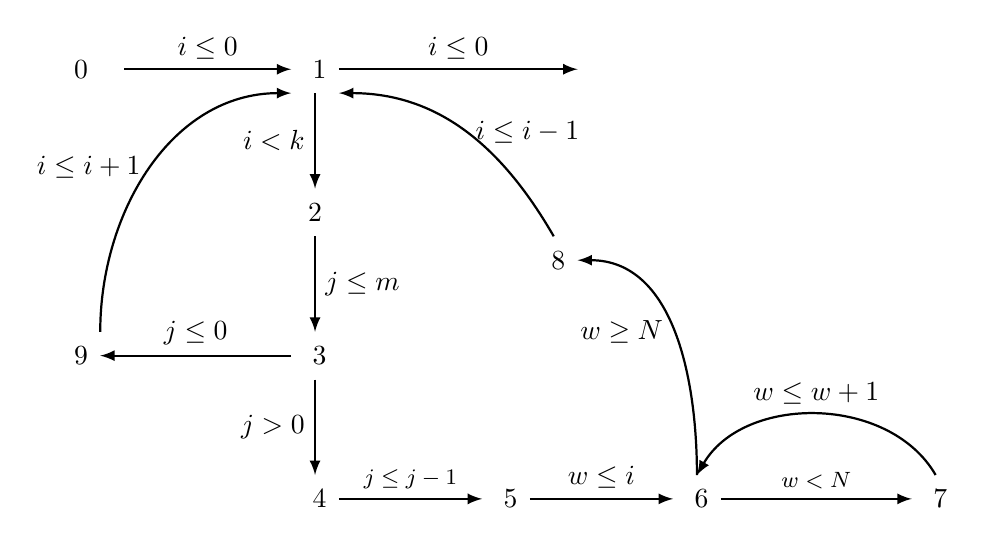
\begin{tikzpicture}[scale=\textwidth/20cm,samples=200]
                \draw[] (-5, 10) circle (0pt) node{{ $0$}};
                \draw[] (0, 10) circle (0pt) node{{ $1$}};
                \draw[] (6, 10) circle (0pt) node {{$\lex$}};
                \draw[] (0, 7) circle (0pt) node{{$2$}};
                \draw[] (0, 4) circle (0pt) node{{ $3$}};
                \draw[] (-5, 4) circle (0pt) node{{ $9$}};
                \draw[] (0, 1) circle (0pt) node{{ $4$}};
                \draw[] (4, 1) circle (0pt) node{{ $5$}};
                \draw[] (8, 1) circle (0pt) node{{ $6$}};
                \draw[] (13, 1) circle (0pt) node{{ $7$}};
                \draw[] (5, 6) circle (0pt) node{{ $8$}};
                % Counter Variables
                %
                % Control Flow Edges:
                \draw[ thick, -latex] (-4, 10)  -- node [above] {$i \leq 0$}(-0.5, 10);
                \draw[ thick, -latex] (0, 9.5)  -- node [left] {$i < k$} (0, 7.5) ;
                \draw[ thick, -latex] (0, 6.5)  -- node [right] {$j \leq m$} (0, 4.5) ;
                \draw[ thick, -latex] (0, 3.5)  -- node [left] {$j > 0$} (0, 1.5) ;
                \draw[ thick, -latex] (-0.5, 4)  -- node [above] {$j \leq 0$} (-4.5, 4) ;
                \draw[ thick, -latex] (-4.5, 4.5)  to  [out=90,in=180]  node [left] {$i \leq i + 1$ }(-0.5, 9.5);
                \draw[ thick, -latex] (0.5, 10)  -- node [above] {$i \leq 0$}  (5.5, 10);
                \draw[ thick, -latex] (0.5, 1)  -- node [above] {{\footnotesize $j \leq j - 1$}}  (3.5, 1);
                \draw[ thick, -latex] (4.5, 1)  -- node [above] {$w \leq i$}  (7.5, 1);
                \draw[ thick, -latex] (8.5, 1)  -- node [above] {{\footnotesize $w < N$}}  (12.5, 1);
                \draw[ thick, -latex] (8, 1.5)  to [out=90,in=0] node [left] {{$w \geq N$}}  (5.5, 6);
                \draw[ thick, -latex] (13, 1.5)  to  [out=120,in=60] node [above] {$w \leq w + 1$}  (8, 1.5);
                \draw[ thick, -latex] (5, 6.5)  to  [out=120,in=0]  node [right] {$i \leq i - 1$ }(0.5, 9.5);
                \end{tikzpicture}
%     \caption{}
%     \end{centering}
%     \end{subfigure}
% \begin{subfigure}{.2\textwidth}    
% \begin{centering}
    {\small
$
    \begin{array}{ll}
        \tpath_0 = (0 \to 1)
        &
        \tpath_4 = (6 \to 8 \to 3)
        \\        
        \tpath_1 = (1 \to 2 \to 3)
        &
        \tpath_5 = (3 \to 9 \to 1)
        \\
        \tpath_2 = (3 \to 4 \to 5 \to 6)
        &
        \tpath_6 = (1 \to \lex)
        \\
        \tpath_3 = (6 \to 7 \to 6)
    \end{array}
$
$
    \begin{array}{l}
        \rprog_1 = {\rprepeat(\tpath_1; 3: {\rprepeat(\tpath_2; 6 : {\rprepeat(\tpath_3)}; \tpath_4)}; \tpath_5)}
        \\
        \rprog_3 = {\rprepeat(\tpath_2; 6 : {\rprepeat(\tpath_3)}; \tpath_4)}
    \end{array}
$
}
\caption{}
\end{centering}
\end{subfigure}
    \caption{
    (a) An example of three nested loops with related iterator variables.
    (b) The abstract transition graph, simple transition paths and loop body.}
        \label{fig:threeWhile-overview}
    \end{figure}

% %

%%%%%%%%%%%%%%%%%%%%%%%%%%%%%%%%%%%%%%%%%%%%%%%%%%%%%%%%%%%%%%%%%%%%%%%%%%%%%%%%%%%%%%%%%%%%%%%%%%%%%%%%%%%%%%%%%%%%%%%%%%%%%%%%%%%%%%%%
%%%%%%%%%%%%%%%%%%%%%%%%%%%%%%%%%%%%%%%%%%%%%%%% The Program Model and Definition %%%%%%%%%%%%%%%%%%%%%%%%%%%%%%%%%%%%%%%%%%%%%%%%%%%%%%%%
%%%%%%%%%%%%%%%%%%%%%%%%%%%%%%%%%%%%%%%%%%%%%%%%%%%%%%%%%%%%%%%%%%%%%%%%%%%%%%%%%%%%%%%%%%%%%%%%%%%%%%%%%%%%%%%%%%%%%%%%%%%%%%%%%%%%%%%%%
\section{Program Model and The Reachability-bound}
\label{sec:preliminary}
% \input{preliminary}
\subsection{Labeled Language}
\[
\begin{array}{llll}
\mbox{Arithmetic Operators} 
& \oplus_a & ::= & + ~|~ - ~|~ \times 
%
~|~ \div ~|~ \emax ~|~ \emin
\\  
\mbox{Arithmetic Expression} 
& \aexpr & ::= & 
n ~|~ {x} ~|~ \aexpr \oplus_a \aexpr  
 ~|~ \elog \aexpr  ~|~ \esign \aexpr
\\
\mbox{Boolean Expression} & \bexpr & ::= & 
%
\etrue ~|~ \efalse  ~|~ \neg \bexpr
 ~|~ \bexpr \land \bexpr
%
~|~ \bexpr \lor \bexpr
~|~ \aexpr \leq \aexpr 
~|~ \aexpr < \aexpr 
~|~ \aexpr = \aexpr 
\\
\mbox{Expression} & \expr & ::= & v ~|~ \aexpr ~|~ \bexpr ~|~ [\expr, \dots, \expr]
\\  
%
\mbox{Value} 
& v & ::= & { n \in \mathbb{N}^{\infty} ~|~ \etrue ~|~ \efalse ~|~ [] ~|~ [v, \dots, v]} \\
%
% \\%
\mbox{Label} 
& l & \in & (\mathbb{N} \cup \{\lin, \lex\}) 
\\ 
%
\mbox{Labeled Command} 
& {c} & ::= &  
\clabel{\assign{x}{\expr}}^l 
~|~  \clabel{\eskip}^l
~|~ \ewhile \clabel{\bexpr}^{l} \edo ({c})
~|~ \eif(\clabel{\bexpr}^{l} , {c}, {c}) 
~|~ {c};{c}  
\\ 
\mbox{Event} 
& \event & ::= & 
({x}, l, v) ~ \mbox{Assignment Event} 
% \\
% &&& 
~|~(\bexpr, l, v) ~ \mbox{Testing Event}
\\
\mbox{Trace} & \trace
& ::= & [] ~|~ \trace :: \event
\\
\end{array}
\]
We denote by $\infty$ a value s.t. $n < \infty $ for all $n \in \mathbb{N}$.
We use following notations to represent the sets of corresponding terms:
\[
\begin{array}{lll}
\vardom & : & \mbox{Set of Variables}  
\\ 
%
\booldom & : & \mbox{Set of Boolean Expressions}  
\\ 
%
\cdom & : & \mbox{Set of Commands} 
\\ 
%
\eventset  & : & \mbox{Set of Events}  
\\
%
\eventset^{\asn}  & : & \mbox{Set of Assignment Events}  
\\
%
\eventset^{\test}  & : & \mbox{Set of Testing Events}  
\\
%
\ldom  & : & \mbox{Set of Labels}  
\\
%
\highlight{\ftdom} & : & \mbox{\highlight{Set of All Finite Execution Traces}}
\\
\highlight{\inftdom} & : & \mbox{\highlight{Set of Infinite  Execution Traces}}
\\
\highlight{\tdom} & : & \mbox{\highlight{Set of All Finite Or Infinite  Execution Traces}}
\\ 
%
\inpvar(c) & : & \mbox{Set of Program $c$'s Input Variables}  
\\
%
\ftdom_0(c) & : & \mbox{Set of Program $c$'s Initial Traces.}
\\ & & \mbox{Each initial trace $\trace_0 \in \ftdom_0(c)$ is finite and every input variable of the program $c$ has an initial value in $\trace_0$.}
\end{array}
\]
%
\subsection{{Trace-based Operational Semantics}}
\label{sec:operational_semantics}
\paragraph{Event}
An event is a triple.
Its first element is the variable name $x$,
or a boolean expression (from the guard of if or while command), 
following by 
 the label, $l$ associated to this command and the value assigned to the variable.

 We have two kinds of events: \emph{assignment events} and \emph{testing events},
 and we use $\eventset^{\asn}$ and $\eventset^{\test}$ to denote the set of all assignment events and testing events, respectively.

 An \emph{assignment event} tracks the execution of an assignment and consists of the assigned variable, the label of the command that generates it, the value assigned to the variable.

 A \emph{testing event} tracks the execution of if and while commands, specifically the evaluation of the boolean expression $b$ in the guard of a $\eif(\clabel{b}^l, c_1, c_2)$ command or $\ewhile \clabel{b}^l \edo c$.
 It consists of the boolean expression $b$ in the guard of the command, the label of the guard, the result of evaluating the guard.
%
\[
\begin{array}{llll}
  \mbox{Event} 
  & \event & ::= & 
  ({x}, l, v) ~ \mbox{Assignment Event} 
  ~|~(\bexpr, l, v) ~ \mbox{Testing Event}
\end{array}
\]
Event projection operators $\pi_i$ projects the $i^{th}$ element from an event: 
% \\
$\pi_i : 
\eventset \to \vardom \cup \booldom \cup \ldom $

\paragraph{Trace.}
%
A trace $\trace \in \tdom $ is a list of events, 
collecting the events generated along the program execution. 
\[
\begin{array}{llll}
\mbox{Trace} & \trace
& ::= & [] ~|~ \trace :: \event
\end{array}
\]
A trace can be regarded as the program history, 
which records all the evaluations for assignment commands and guards in $\eif$ and $\ewhile$ command.
\\
\highlight{If a program doesn't terminate when executing under some initial trace, it produces an infinite trace $\trace \in \tdom^{\infty}$.
$\tdom^{\infty}$ is the set of all finite or infinite traces.}
\\
$\tracecat: \mathcal{T} \to \mathcal{T} \to \mathcal{T}$ is the trace concatenation operator, which combines two traces,
and $\vcounter : \mathcal{T} \to \mathbb{N} \to \mathbb{N}$ is the counting operator, 
which counts the occurrence of a labeled variable in the trace. When the input trace is infinite, it returns $\infty$.
$\event \in \trace $ or $\event \notin \trace $ denotes that $\event$ belongs to $trace$ or not.
All the definition details are in the appendix.
%
The counter operator is abused when the input is a sequence of labels $L = (l_1, \cdots, l_n)$ by counting the occurrence
of this sequence in trace. Specifically,
$\vcounter(\trace :: (\_, l_1, \_) :: \cdots :: (\_, l_n, \_), L ) \triangleq \vcounter(\trace, L) + 1$
and $\vcounter(\trace :: (\_, l, \_), L ) 
\triangleq \vcounter(\trace, L) ~ l \neq l_n$, etc.
The operator $\tlabel : \tdom \to \mathcal{P}{(\ldom)}$ gives the set of labels in every event belonging to a trace.
$\tlabel{(\trace  :: (\_, l, \_)])} \triangleq \{l\} \cup \tlabel{(\trace )}$ and $\tlabel({[ ]}) \triangleq \{\}$.
%
\paragraph{Environment.} $\env : {\ftdom}  \to \vardom \to(\mathbb{N} \cup \{\bot\})$
\[
\begin{array}{llll}
\env(\trace  \traceadd (x, l, v)) x \triangleq v
&
\env(\trace \traceadd (y, l, v)) x \triangleq \env(\trace) x, y \neq x
&
\env(\trace \traceadd (b, l, v)) x \triangleq \env(\trace) x
&
\env({[]} ) x \triangleq \bot
\end{array}
\]
%
\begin{lem}[Initial Traces]
  \label{lem:initial_trace}
  \[
    \forall c \in \cdom, \trace \in \ftdom \st \trace \in \ftdom_0(c) \iff 
    \forall x \in \inpvar(c) \st \env(\trace_0) x \neq \bot
    \]
\end{lem}
%
\paragraph{Configuration.}
%
\paragraph{Expression Semantics}
The evaluation notation for arithmetic expression is $\econfig{} : \mathcal{A} \to \tdom \to \mathcal{V}$.
The $\econfig{\aexpr}(\trace)$ evaluates an arithmetic expression $\aexpr$ under trace $\trace$ following the arithmetic expression evaluation rules in Figure~\ref{fig:aexpr-eval}.
\begin{figure}
\begin{mathpar}
  \boxed{ \econfig{} \, : \, \mbox{Arithmetic Expression $\to$ Trace $\to$ Arithmetic Value}}
  \\
  \inferrule{ 
    \empty
  }{
   \econfig{n} (\trace)
   = n
  }
  \and
  \inferrule{ 
    \env(\trace) x = v
  }{
   \econfig{x} 
   = v
  }
  \and
  \inferrule{ 
    \econfig{\aexpr_1}(\trace) = v_1
    \and 
    \econfig{\aexpr_2}(\trace) = v_2
    \and 
     v_1 \oplus_a v_2 = v
  }{
   \econfig{\aexpr_1 \oplus_a \aexpr_2} 
   = v
  }
  \and
  \inferrule{ 
    \econfig{\aexpr}(\trace) = v'
    \and 
    \elog v' = v
  }{
   \econfig{\elog \aexpr}(\trace) 
   = v
  }
  \and
  \inferrule{ 
    \econfig{\aexpr}(\trace) = v'
    \and 
    \esign v' = v
  }{
   \econfig{\esign \aexpr} 
   = v
  }
   \end{mathpar}
   \caption{Evaluation Rules of Arithmetic Expression}
   \label{fig:aexpr-eval}
   \end{figure}

 The evaluation rules for boolean expression and standard expression are in Figure~\ref{fig:bexpr-eval} and Figure~\ref{fig:expr-eval}.
 \begin{figure}
  \begin{mathpar}
  \boxed{ \barrow \, : \, \mbox{ Boolean Expression $\times$ Trace $\rightarrow$ Boolean Value} }
  \\
  \inferrule{ 
    \empty
  }{
   \config{\efalse, \trace} 
   \barrow \efalse
  }
  \and 
  \inferrule{ 
    \empty
  }{
   \config{\etrue, \trace} 
   \barrow \etrue
  }
  \and 
  \inferrule{ 
    \config{\bexpr, \trace} \barrow v'
    \and 
    \neg v' = v
  }{
   \config{\neg \bexpr, \trace} 
   \barrow v
  }
  \and 
  \inferrule{ 
    \config{\bexpr, \trace_1} \barrow v_1
    \and 
    \config{\bexpr, \trace_2} \barrow v_2
    \and 
     v_1 \land v_2 = v
  }{
   \config{\bexpr, \trace_1 \land \bexpr_2} 
   \barrow v
  }
  \and 
  \inferrule{ 
    \config{\bexpr, \trace_1} \barrow v_1
    \and 
    \config{\bexpr, \trace_2} \barrow v_2
    \and 
     v_1 \lor v_2 = v
  }{
   \config{\bexpr, \trace_1 \lor \bexpr_2} 
   \barrow v
  }
  \end{mathpar}
  \caption{Evaluation Rules of Boolean Expression}
  \label{fig:bexpr-eval}
  \end{figure}
  
  \begin{figure}
    \begin{mathpar}
  \boxed{ \earrow \, : \, \mbox{Expression $\times$ Trace $\rightarrow$ Value} }
  \\
  \inferrule{ 
    \econfig{\aexpr}(\trace) = v
  }{
   \config{\aexpr, \trace} 
   \earrow v
  }
  \and
  \inferrule{ 
    \config{\bexpr, \trace} \barrow v
  }{
   \config{\bexpr, \trace} 
   \earrow v
  }
  \and
  \inferrule{ 
    \config{\expr_1, \trace} \earrow v_1
    \cdots
    \config{\expr_n, \trace} \earrow v_n
  }{
   \config{ [\expr_1, \cdots, \expr_n], \trace} 
   \earrow [v_1, \cdots, v_n]
  }
  \and
  \inferrule{ 
    \empty
  }{
   \config{v, \trace} 
   \earrow v
  }
   \end{mathpar}
   \caption{Evaluation Rules of Standard Expression}
   \label{fig:expr-eval}
   \end{figure}

\paragraph{Operational Semantics Rules}
%
The trace based operational semantics rules are defined as in Figure~\ref{fig:command-os}.
\begin{figure}
  \begin{mathpar}
\boxed{
\mbox{Command $\times$ Trace}
\xrightarrow{}
\mbox{Command $\times$ Trace}
}
\and
\boxed{\config{{c, \trace}}
\xrightarrow{} 
\config{{c',  \trace'}}
}
%
\\
%
\inferrule
{
\config{\expr, \trace} \earrow v
  \and
\event = ({x}, l, v)
}
{
\config{\clabel{\assign{{x}}{\expr}}^{l},  \trace } 
\xrightarrow{} 
\config{\clabel{\eskip}^l, \trace \traceadd \event}
}
~\rname{assn}
\and
%
\inferrule
{
  \config{\bexpr, \trace} \earrow \etrue
 \and 
 \event = (\bexpr, l, \etrue)
}
{
\config{{\ewhile \clabel{\bexpr}^{l} \edo (c), \trace}}
\xrightarrow{} 
\config{{
c; \ewhile \clabel{\bexpr}^{l} \edo (c),
\trace \traceadd \event}}
}
~\rname{while-t}
%
%
\and
%
\inferrule
{
  \config{\bexpr, \trace} \earrow \efalse
 \and 
 \event = (\bexpr, l, \efalse)
}
{
\config{{\ewhile \clabel{\bexpr}^{l} \edo (c), \trace}}
\xrightarrow{} 
\config{{
  \clabel{\eskip}^l,
\trace \traceadd \event}}
}
~\rname{while-f}
%
%
\and
%
%
\inferrule
{
\config{{c_1, \trace}}
\xrightarrow{}
\config{{c_1',  \trace'}}
}
{
\config{{c_1; c_2, \trace}} 
\xrightarrow{} 
\config{{c_1'; c_2, \trace'}}
}
~\rname{seq1}
%
\and
%
\inferrule
{
  \config{{c_2, \trace}}
  \xrightarrow{}
  \config{{c_2',  \trace'}}
}
{
\config{{\clabel{\eskip}^l; c_2, \trace}} \xrightarrow{} \config{{ c_2', \trace'}}
}
~\rname{seq2}
%
\and
%
%
\inferrule
{
  \config{\bexpr, \trace} \earrow \etrue
 \and 
 \event = (\bexpr, l, \etrue)
}
{
\config{{
\eif(\clabel{\bexpr}^{l}, c_1, c_2), 
\trace}}
\xrightarrow{} 
\config{{c_1, \trace \traceadd \event}}
}
~\rname{if-t}
%
\and
%
\inferrule
{
 \config{\bexpr, \trace} \earrow \efalse
 \and 
 \event = (\bexpr, l, \efalse)
}
{
\config{{\eif(\clabel{\bexpr}^{l}, c_1, c_2), \trace}}
\xrightarrow{} 
\config{{c_2, \trace \traceadd \event}}
}
~\rname{if-f}
%
\end{mathpar}
\caption{Operational Semantics Rules}
\label{fig:command-os}
\end{figure}


Given an initial trace $\trace_0 \in \ftdom_0(c)$ of the program $c$,
we use $\to^*$ for the reflexive and transitive closure of $\to$. 
If $\config{c, \trace_0} \rightarrow^{*} \config{\clabel{\eskip}^l, \trace_0 \tracecat \trace}$,
then the program's execution terminates and produces a finite execution trace $\trace \in \ftdom$.
\\
\begin{defn}[Non-terminating and Infinite Trace]
  \label{def:non-terminating}
  Given a program $c$ and an initial trace $\trace \in \ftdom_0(c)$,
  when $c$ executes with $\trace$,  we define the execution of $c$ under $\trace$ is non-terminating and produces an infinite trace $\trace' \in \inftdom$, as 
  $\config{c, \trace_0} \uparrow^{\infty} \trace' \in \lim(\uparrow)$
  where the limit is defined as follows.
  \[
    \begin{array}{l}
      \lim(\uparrow) 
      % \in \left( (\cdom \times \ftdom) \times (\cdom \times \inftdom) \right) 
      \triangleq 
    \\ \quad
    \Big\{
      (\config{c, \trace}, \trace') ~\vert~ 
      c\in \cdom, \trace \in \ftdom_0(c),
      \trace' \in \inftdom 
      \land \exists \trace_0 \in \ftdom, c_0 \in \cdom \st 
      \config{c, \trace} \to \config{c_0, \trace_0}
      \\ \qquad \qquad \qquad 
      \land \forall i \in \mathbb{N}, \exists \trace_i, \trace_{i + 1} \in \ftdom, \trace'' \in \inftdom, c_i, c_{i + 1} \in \cdom \st 
      \config{c_i, \trace_i} \to \config{c_{i + 1}, \trace_{i + 1}} 
      \land  \trace' = \trace_{i + 1} \tracecat \trace''
    \Big\}
    \end{array}
  \]
\end{defn}
%
% \begin{defn}[Non-terminating and Infinite Trace (alternative way)]
%   \label{def:non-terminating-2}
%   Given a program $c$ and an initial trace $\trace_0 \in \ftdom_0(c)$,
%   when $c$ executes with $\trace_0$,  we define $c$ is non-terminating under $\trace_0$, $\config{c, \trace_0} \uparrow^{\infty}$ if and only if there exists a function
%   $f : \mathbb{N} \to \cdom \times \tdom$ such that $f(0) = \config{c, \trace_0}$ and
%   for every $i \in \mathbb{N}$ there exist  $\trace_i, \trace_{i + 1}\in \tdom$, $c_i, c_{i + 1} \in \cdom$ such that  $f(i) = \config{c_i, \trace_i}$, $f(i + 1) =  \config{c_{i + 1}, \trace_{i + 1}}$ and
%   $\config{c_i, \trace_i} \to \config{c_{i + 1}, \trace_{i + 1}}$. 
%   \[
%     \begin{array}{l}
%     \forall \trace_0 \in \ftdom_0(c), c \in \cdom \st
%     \config{c, \trace_0} \uparrow^{\infty}
%     \\
%     \iff \exists f : \mathbb{N} \to \cdom \times \tdom \st 
%     f(0) = \config{c, \trace_0}
%     \\ \qquad \land
%     \forall i \in \mathbb{N}, \exists \trace_i, \trace_{i + 1} \in \tdom, c_i, c_{i + 1} \in \cdom\st 
%     \\ \qquad \quad
%     f(i) = \config{c_i, \trace_i}$, $f(i + 1) =  \config{c_{i + 1}, \trace_{i + 1}} \land \config{c_i, \trace_i} \to \config{c_{i + 1}, \trace_{i + 1}}
%     \end{array}
%   \]
%   Given a program $c$ and an initial trace $\trace_0 \in \ftdom_0(c)$, if $\config{c, \trace_0} \uparrow^{\infty}$, 
%   let $f$ be the function such that for every $i \in \mathbb{N}$,  $\trace_i, \trace_{i + 1}\in \tdom$, $c_i, c_{i + 1} \in \cdom$ where $\config{c_i, \trace_i} \to \config{c_{i + 1}, \trace_{i + 1}}$, we have $f(i) = \config{c_i, \trace_i}$, $f(i + 1) =  \config{c_{i + 1}, \trace_{i + 1}}$. 
%   Let $\pi_2 : (\cdom \times \tdom) \to \tdom$ be the projector which projects the trace from a configuration,
%   then we define $\config{c, \trace_0} \uparrow^{\infty} \trace'$ produces an infinite trace $\trace' = \pi_2(\lim\limits_{i \to \infty}(f(i))) \in \inftdom$.
%   \[ \trace' = \lim( \pi_2 \circ (f(i))). \]
% \end{defn}
% %

% \begin{defn}[Non-terminating and Infinite Trace (third way)]
%   \label{def:infinite-trace}
%   Given a program $c$ and an initial trace $\trace_0 \in \ftdom_0(c)$,
%   when $c$ executes with $\trace_0$,  we define $c$ is non-terminating under $\trace_0$, denoted as $\config{c, \trace_0} \uparrow^{\infty} \trace'$ and produce an infinite trace $\trace' \in \inftdom$ 
%   if and only if there exists a function
%   $f : \mathbb{N} \to \cdom \times \tdom$ such that $f(0) = \config{c, \trace_0}$ and
%   for every $i \in \mathbb{N}$ there exist  $\trace_i, \trace_{i + 1}\in \tdom$, $c_i, c_{i + 1} \in \cdom$ such that  $f(i) = \config{c_i, \trace_i}$, $f(i + 1) =  \config{c_{i + 1}, \trace_{i + 1}}$ and
%   $\config{c_i, \trace_i} \to \config{c_{i + 1}, \trace_{i + 1}}$. 
%   \[
%     \begin{array}{l}
%     \forall \trace_0 \in \ftdom_0(c), \trace' \in \inftdom, c \in \cdom \st
%     \config{c, \trace_0} \uparrow^{\infty} \trace'
%     \\
%     \iff \exists f : \mathbb{N} \to \cdom \times \tdom \st 
%     f(0) = \config{c, \trace_0}
%     \\ \qquad \land
%     \forall i \in \mathbb{N}, \exists \trace_i, \trace_{i + 1} \in \tdom, c_i, c_{i + 1} \in \cdom\st 
%     \\ \qquad \quad
%     f(i) = \config{c_i, \trace_i}$, $f(i + 1) =  \config{c_{i + 1}, \trace_{i + 1}} \land \config{c_i, \trace_i} \to \config{c_{i + 1}, \trace_{i + 1}}.
%     \end{array}
%   \]
%   Let $\pi_2 : (\cdom \times \tdom) \to \tdom$ be the projector which projects the trace from a configuration,
%   then the infinite trace $\trace'$ produced by $\config{c, \trace_0} \uparrow^{\infty} \trace'$ is
%   \[ \trace' = \pi_2(\lim\limits_{i \to \infty}(f(i))) \in \inftdom. \]
% \end{defn}
%
This follows the maximal trace semantics in \cite{cousot2019abstract} Section 2.5 Equation (12).
\\
If we observe the operational semantics rules, we can find that no rule will shrink the trace. 
So we have the Lemma~\ref{lem:tracenondec} with proof in Appendix~\ref{apdx:lem_language}, 
specifically the trace has the property that its length never decreases during the program execution.
\begin{lem}
  [Trace Non-Decreasing]
  \label{lem:tracenondec}
  For any program $c \in \cdom$ and initial trace $\trace_0 \in \ftdom_0(c)$,
  if there exists $\trace \in \tdom$ and $c' \in \cdom $ such that $\config{c, \trace_0} \rightarrow^{*} \config{c', \trace} $ or 
  $\config{c, \trace_0} \uparrow^{\infty} \trace$  
  then there exists a trace $\trace' \in \tdom$ such that $\trace_0 \tracecat \trace' = \trace$ formally as follows.
  %
  \[
    \begin{array}{l}
    \forall \trace_0 \in \ftdom_0(c), \trace \in \tdom, c, c' \in \cdom \st
    \Big( \config{c, \trace_0} \rightarrow^{*} \config{c', \trace} 
    \lor  \config{c, \trace_0} \uparrow^{\infty} \trace \Big)
    \\ \quad
    \implies \exists \trace' \in \tdom \st \trace_0 \tracecat \trace' = \trace 
    \end{array}
    \]
  \end{lem}
  % \begin{lem}
  %   [Trace Non-Decreasing (based on the alternative non-termination definition)]
  %   \label{lem:tracenondec2}
  %   For any program $c \in \cdom$ and initial trace $\trace_0 \in \ftdom_0(c)$,
  %   \begin{itemize}
  %     \item if there exists $\trace \in \tdom$ and $c' \in \cdom $ such that $\config{c, \trace_0} \rightarrow^{*} \config{c', \trace} $
  %     then there exists a trace $\trace' \in \ftdom$ such that $\trace_0 \tracecat \trace' = \trace$;
  %     \item if $\config{c, \trace_0} \uparrow^{\infty} $ and produces an infinite trace $\trace \in \inftdom$ as defined in Definition~\ref{def:non-terminating}
  %     then there exists an infinite trace $\trace' \in \inftdom$ such that $\trace_0 \tracecat \trace' = \trace$ formally as follows.  
  %   \end{itemize}
  %   %
  %   \[
  %     \begin{array}{l}
  %     \forall \trace_0 \in \ftdom_0(c), \trace \in \tdom, c, c' \in \cdom \st
  %     \config{c, \trace_0} \rightarrow^{*} \config{c', \trace} 
  %     \implies \exists \trace' \in \ftdom \st \trace_0 \tracecat \trace' = \trace 
  %     \\
  %     \todomath{\land \config{c, \trace_0} \uparrow^{\infty} \implies \exists \trace' \in \inftdom \st \trace_0 \tracecat \trace' \in \inftdom}
  %     \end{array}
  %     \]
  %   \end{lem}

\emph{The Reachability-bound}

\mg{I am looking at the definition of reachability bound and the different measures involved. I don’t think it make sense to have 0 for an infinite trace. I actually find the formalization of the diverging cases quite unclear. suppose we change the definition to have that the reachability-bound for a non-terminating program to be infinite, is the program analysis still sound?}

We first introduce two important counter notations counting the occurrence of a program point and a list of program points respectively.
\begin{defn}[Program Point Counter]
 \label{def:counter}
The counting operator $\counter : \tdom \to \ldom \to \mathbb{N}$
counts the appearance of a label in a trace.
\begin{center}
{\small
$
\begin{array}{llll}
\counter([(\_, l, v)] \tracecat \trace', l ) \triangleq \counter(\trace', l) + 1 & \text{if}~ l = l
&
\counter({[]}, l) \triangleq 0 & 
\\
\counter([(\_, l', v)] \tracecat \trace', l) \triangleq \counter(\trace', l) & \text{if}~ l' \neq l
&
\counter(\trace, l) \triangleq 0 & \text{if }~ \trace \in \inftdom
\end{array}
$
}
\end{center}
\end{defn}
\begin{defn}[Point List Counter]
 \label{def:lcounter}
 The counting operator $\lcounter : \tdom \to \mathcal{P}(\ldom) \to \mathbb{N}$
 counts the appearance of a list of labels $L = [l_1, \ldots, l_n]$ as
{\small
\begin{center}
 $
 \begin{array}{lll}
 \lcounter(\trace'' \tracecat \trace', L ) 
 & \triangleq \lcounter(\trace', L) + 1 & \text{if}~ \pi_2(\trace''[i]) = l_i, \forall i = 1, \ldots, n
 \\ 
 \lcounter([(\_, l, \_)] \tracecat \trace'' \tracecat \trace', L ) 
 & \triangleq \lcounter(\trace', L) & \text{if}~ l \neq l_1 \lor \bigvee\limits_{i = 2, \ldots, n} \pi_2(\trace''[i]) \neq l_i
 \\ 
 \lcounter(\trace, L ) 
 & \triangleq 0 & \text{if }~ \trace \in \inftdom.
 \end{array}
 $
 \end{center}
 }
% {When the input trace is infinite, $\lcounter(\trace, L)$ returns $\bot$ for any $L$.}
\end{defn}
%
When the input trace is infinite, both $\counter(\trace, l)$ and $\lcounter(\trace, L)$ returns $0$.
We denote by $\infty$ a value s.t. $v < \infty $ for all $v \in \mathbb{N}$

\begin{defn}[Reachability-bound]
 \label{def:rb}
 For a program ${c}$ and a location $l$ in $c$,
a function $f(c, l) : \tdom \to (\mathbb{N} \cup \{\infty\})$ is a \emph{reachability-bound} for $l$ if and only if
{\small
\begin{center}
 $
\begin{array}{ll}
 \forall \trace_0 \in \ftdom_0(c), \trace \in \tdom, c' \in \cdom, l, l' \in \lvar(c) \st 
 \\ \qquad
 \Big(
 \config{{c}, \trace_0} \to^{*} \config{\clabel{\eskip}^{l'}, \trace_0 \tracecat \trace} 
 \lor 
 \config{{c}, \trace_0} \uparrow^{\infty} \trace_0 \tracecat \trace 
 \Big)
 \implies f({c}, l)(\trace_0) \geq \counter(\trace, l) 
 \end{array}
 $
\end{center}
}
\end{defn}
It is easy to compute a trivial \emph{reachability-bound} $f(c, l): \tdom \to \infty$, and 
our algorithm computes a non-trivial one.


% \section{{Language and Program Model}}
% \label{sec:language}
% \subsection{Labeled Language}
\[
\begin{array}{llll}
\mbox{Arithmetic Operators} 
& \oplus_a & ::= & + ~|~ - ~|~ \times 
%
~|~ \div ~|~ \emax ~|~ \emin
\\  
\mbox{Arithmetic Expression} 
& \aexpr & ::= & 
n ~|~ {x} ~|~ \aexpr \oplus_a \aexpr  
 ~|~ \elog \aexpr  ~|~ \esign \aexpr
\\
\mbox{Boolean Expression} & \bexpr & ::= & 
%
\etrue ~|~ \efalse  ~|~ \neg \bexpr
 ~|~ \bexpr \land \bexpr
%
~|~ \bexpr \lor \bexpr
~|~ \aexpr \leq \aexpr 
~|~ \aexpr < \aexpr 
~|~ \aexpr = \aexpr 
\\
\mbox{Expression} & \expr & ::= & v ~|~ \aexpr ~|~ \bexpr ~|~ [\expr, \dots, \expr]
\\  
%
\mbox{Value} 
& v & ::= & { n \in \mathbb{N}^{\infty} ~|~ \etrue ~|~ \efalse ~|~ [] ~|~ [v, \dots, v]} \\
%
% \\%
\mbox{Label} 
& l & \in & (\mathbb{N} \cup \{\lin, \lex\}) 
\\ 
%
\mbox{Labeled Command} 
& {c} & ::= &  
\clabel{\assign{x}{\expr}}^l 
~|~  \clabel{\eskip}^l
~|~ \ewhile \clabel{\bexpr}^{l} \edo ({c})
~|~ \eif(\clabel{\bexpr}^{l} , {c}, {c}) 
~|~ {c};{c}  
\\ 
\mbox{Event} 
& \event & ::= & 
({x}, l, v) ~ \mbox{Assignment Event} 
% \\
% &&& 
~|~(\bexpr, l, v) ~ \mbox{Testing Event}
\\
\mbox{Trace} & \trace
& ::= & [] ~|~ \trace :: \event
\\
\end{array}
\]
We denote by $\infty$ a value s.t. $n < \infty $ for all $n \in \mathbb{N}$.
We use following notations to represent the sets of corresponding terms:
\[
\begin{array}{lll}
\vardom & : & \mbox{Set of Variables}  
\\ 
%
\booldom & : & \mbox{Set of Boolean Expressions}  
\\ 
%
\cdom & : & \mbox{Set of Commands} 
\\ 
%
\eventset  & : & \mbox{Set of Events}  
\\
%
\eventset^{\asn}  & : & \mbox{Set of Assignment Events}  
\\
%
\eventset^{\test}  & : & \mbox{Set of Testing Events}  
\\
%
\ldom  & : & \mbox{Set of Labels}  
\\
%
\highlight{\ftdom} & : & \mbox{\highlight{Set of All Finite Execution Traces}}
\\
\highlight{\inftdom} & : & \mbox{\highlight{Set of Infinite  Execution Traces}}
\\
\highlight{\tdom} & : & \mbox{\highlight{Set of All Finite Or Infinite  Execution Traces}}
\\ 
%
\inpvar(c) & : & \mbox{Set of Program $c$'s Input Variables}  
\\
%
\ftdom_0(c) & : & \mbox{Set of Program $c$'s Initial Traces.}
\\ & & \mbox{Each initial trace $\trace_0 \in \ftdom_0(c)$ is finite and every input variable of the program $c$ has an initial value in $\trace_0$.}
\end{array}
\]
%
\subsection{{Trace-based Operational Semantics}}
\label{sec:operational_semantics}
\paragraph{Event}
An event is a triple.
Its first element is the variable name $x$,
or a boolean expression (from the guard of if or while command), 
following by 
 the label, $l$ associated to this command and the value assigned to the variable.

 We have two kinds of events: \emph{assignment events} and \emph{testing events},
 and we use $\eventset^{\asn}$ and $\eventset^{\test}$ to denote the set of all assignment events and testing events, respectively.

 An \emph{assignment event} tracks the execution of an assignment and consists of the assigned variable, the label of the command that generates it, the value assigned to the variable.

 A \emph{testing event} tracks the execution of if and while commands, specifically the evaluation of the boolean expression $b$ in the guard of a $\eif(\clabel{b}^l, c_1, c_2)$ command or $\ewhile \clabel{b}^l \edo c$.
 It consists of the boolean expression $b$ in the guard of the command, the label of the guard, the result of evaluating the guard.
%
\[
\begin{array}{llll}
  \mbox{Event} 
  & \event & ::= & 
  ({x}, l, v) ~ \mbox{Assignment Event} 
  ~|~(\bexpr, l, v) ~ \mbox{Testing Event}
\end{array}
\]
Event projection operators $\pi_i$ projects the $i^{th}$ element from an event: 
% \\
$\pi_i : 
\eventset \to \vardom \cup \booldom \cup \ldom $

\paragraph{Trace.}
%
A trace $\trace \in \tdom $ is a list of events, 
collecting the events generated along the program execution. 
\[
\begin{array}{llll}
\mbox{Trace} & \trace
& ::= & [] ~|~ \trace :: \event
\end{array}
\]
A trace can be regarded as the program history, 
which records all the evaluations for assignment commands and guards in $\eif$ and $\ewhile$ command.
\\
\highlight{If a program doesn't terminate when executing under some initial trace, it produces an infinite trace $\trace \in \tdom^{\infty}$.
$\tdom^{\infty}$ is the set of all finite or infinite traces.}
\\
$\tracecat: \mathcal{T} \to \mathcal{T} \to \mathcal{T}$ is the trace concatenation operator, which combines two traces,
and $\vcounter : \mathcal{T} \to \mathbb{N} \to \mathbb{N}$ is the counting operator, 
which counts the occurrence of a labeled variable in the trace. When the input trace is infinite, it returns $\infty$.
$\event \in \trace $ or $\event \notin \trace $ denotes that $\event$ belongs to $trace$ or not.
All the definition details are in the appendix.
%
The counter operator is abused when the input is a sequence of labels $L = (l_1, \cdots, l_n)$ by counting the occurrence
of this sequence in trace. Specifically,
$\vcounter(\trace :: (\_, l_1, \_) :: \cdots :: (\_, l_n, \_), L ) \triangleq \vcounter(\trace, L) + 1$
and $\vcounter(\trace :: (\_, l, \_), L ) 
\triangleq \vcounter(\trace, L) ~ l \neq l_n$, etc.
The operator $\tlabel : \tdom \to \mathcal{P}{(\ldom)}$ gives the set of labels in every event belonging to a trace.
$\tlabel{(\trace  :: (\_, l, \_)])} \triangleq \{l\} \cup \tlabel{(\trace )}$ and $\tlabel({[ ]}) \triangleq \{\}$.
%
\paragraph{Environment.} $\env : {\ftdom}  \to \vardom \to(\mathbb{N} \cup \{\bot\})$
\[
\begin{array}{llll}
\env(\trace  \traceadd (x, l, v)) x \triangleq v
&
\env(\trace \traceadd (y, l, v)) x \triangleq \env(\trace) x, y \neq x
&
\env(\trace \traceadd (b, l, v)) x \triangleq \env(\trace) x
&
\env({[]} ) x \triangleq \bot
\end{array}
\]
%
\begin{lem}[Initial Traces]
  \label{lem:initial_trace}
  \[
    \forall c \in \cdom, \trace \in \ftdom \st \trace \in \ftdom_0(c) \iff 
    \forall x \in \inpvar(c) \st \env(\trace_0) x \neq \bot
    \]
\end{lem}
%
\paragraph{Configuration.}
%
\paragraph{Expression Semantics}
The evaluation notation for arithmetic expression is $\econfig{} : \mathcal{A} \to \tdom \to \mathcal{V}$.
The $\econfig{\aexpr}(\trace)$ evaluates an arithmetic expression $\aexpr$ under trace $\trace$ following the arithmetic expression evaluation rules in Figure~\ref{fig:aexpr-eval}.
\begin{figure}
\begin{mathpar}
  \boxed{ \econfig{} \, : \, \mbox{Arithmetic Expression $\to$ Trace $\to$ Arithmetic Value}}
  \\
  \inferrule{ 
    \empty
  }{
   \econfig{n} (\trace)
   = n
  }
  \and
  \inferrule{ 
    \env(\trace) x = v
  }{
   \econfig{x} 
   = v
  }
  \and
  \inferrule{ 
    \econfig{\aexpr_1}(\trace) = v_1
    \and 
    \econfig{\aexpr_2}(\trace) = v_2
    \and 
     v_1 \oplus_a v_2 = v
  }{
   \econfig{\aexpr_1 \oplus_a \aexpr_2} 
   = v
  }
  \and
  \inferrule{ 
    \econfig{\aexpr}(\trace) = v'
    \and 
    \elog v' = v
  }{
   \econfig{\elog \aexpr}(\trace) 
   = v
  }
  \and
  \inferrule{ 
    \econfig{\aexpr}(\trace) = v'
    \and 
    \esign v' = v
  }{
   \econfig{\esign \aexpr} 
   = v
  }
   \end{mathpar}
   \caption{Evaluation Rules of Arithmetic Expression}
   \label{fig:aexpr-eval}
   \end{figure}

 The evaluation rules for boolean expression and standard expression are in Figure~\ref{fig:bexpr-eval} and Figure~\ref{fig:expr-eval}.
 \begin{figure}
  \begin{mathpar}
  \boxed{ \barrow \, : \, \mbox{ Boolean Expression $\times$ Trace $\rightarrow$ Boolean Value} }
  \\
  \inferrule{ 
    \empty
  }{
   \config{\efalse, \trace} 
   \barrow \efalse
  }
  \and 
  \inferrule{ 
    \empty
  }{
   \config{\etrue, \trace} 
   \barrow \etrue
  }
  \and 
  \inferrule{ 
    \config{\bexpr, \trace} \barrow v'
    \and 
    \neg v' = v
  }{
   \config{\neg \bexpr, \trace} 
   \barrow v
  }
  \and 
  \inferrule{ 
    \config{\bexpr, \trace_1} \barrow v_1
    \and 
    \config{\bexpr, \trace_2} \barrow v_2
    \and 
     v_1 \land v_2 = v
  }{
   \config{\bexpr, \trace_1 \land \bexpr_2} 
   \barrow v
  }
  \and 
  \inferrule{ 
    \config{\bexpr, \trace_1} \barrow v_1
    \and 
    \config{\bexpr, \trace_2} \barrow v_2
    \and 
     v_1 \lor v_2 = v
  }{
   \config{\bexpr, \trace_1 \lor \bexpr_2} 
   \barrow v
  }
  \end{mathpar}
  \caption{Evaluation Rules of Boolean Expression}
  \label{fig:bexpr-eval}
  \end{figure}
  
  \begin{figure}
    \begin{mathpar}
  \boxed{ \earrow \, : \, \mbox{Expression $\times$ Trace $\rightarrow$ Value} }
  \\
  \inferrule{ 
    \econfig{\aexpr}(\trace) = v
  }{
   \config{\aexpr, \trace} 
   \earrow v
  }
  \and
  \inferrule{ 
    \config{\bexpr, \trace} \barrow v
  }{
   \config{\bexpr, \trace} 
   \earrow v
  }
  \and
  \inferrule{ 
    \config{\expr_1, \trace} \earrow v_1
    \cdots
    \config{\expr_n, \trace} \earrow v_n
  }{
   \config{ [\expr_1, \cdots, \expr_n], \trace} 
   \earrow [v_1, \cdots, v_n]
  }
  \and
  \inferrule{ 
    \empty
  }{
   \config{v, \trace} 
   \earrow v
  }
   \end{mathpar}
   \caption{Evaluation Rules of Standard Expression}
   \label{fig:expr-eval}
   \end{figure}

\paragraph{Operational Semantics Rules}
%
The trace based operational semantics rules are defined as in Figure~\ref{fig:command-os}.
\begin{figure}
  \begin{mathpar}
\boxed{
\mbox{Command $\times$ Trace}
\xrightarrow{}
\mbox{Command $\times$ Trace}
}
\and
\boxed{\config{{c, \trace}}
\xrightarrow{} 
\config{{c',  \trace'}}
}
%
\\
%
\inferrule
{
\config{\expr, \trace} \earrow v
  \and
\event = ({x}, l, v)
}
{
\config{\clabel{\assign{{x}}{\expr}}^{l},  \trace } 
\xrightarrow{} 
\config{\clabel{\eskip}^l, \trace \traceadd \event}
}
~\rname{assn}
\and
%
\inferrule
{
  \config{\bexpr, \trace} \earrow \etrue
 \and 
 \event = (\bexpr, l, \etrue)
}
{
\config{{\ewhile \clabel{\bexpr}^{l} \edo (c), \trace}}
\xrightarrow{} 
\config{{
c; \ewhile \clabel{\bexpr}^{l} \edo (c),
\trace \traceadd \event}}
}
~\rname{while-t}
%
%
\and
%
\inferrule
{
  \config{\bexpr, \trace} \earrow \efalse
 \and 
 \event = (\bexpr, l, \efalse)
}
{
\config{{\ewhile \clabel{\bexpr}^{l} \edo (c), \trace}}
\xrightarrow{} 
\config{{
  \clabel{\eskip}^l,
\trace \traceadd \event}}
}
~\rname{while-f}
%
%
\and
%
%
\inferrule
{
\config{{c_1, \trace}}
\xrightarrow{}
\config{{c_1',  \trace'}}
}
{
\config{{c_1; c_2, \trace}} 
\xrightarrow{} 
\config{{c_1'; c_2, \trace'}}
}
~\rname{seq1}
%
\and
%
\inferrule
{
  \config{{c_2, \trace}}
  \xrightarrow{}
  \config{{c_2',  \trace'}}
}
{
\config{{\clabel{\eskip}^l; c_2, \trace}} \xrightarrow{} \config{{ c_2', \trace'}}
}
~\rname{seq2}
%
\and
%
%
\inferrule
{
  \config{\bexpr, \trace} \earrow \etrue
 \and 
 \event = (\bexpr, l, \etrue)
}
{
\config{{
\eif(\clabel{\bexpr}^{l}, c_1, c_2), 
\trace}}
\xrightarrow{} 
\config{{c_1, \trace \traceadd \event}}
}
~\rname{if-t}
%
\and
%
\inferrule
{
 \config{\bexpr, \trace} \earrow \efalse
 \and 
 \event = (\bexpr, l, \efalse)
}
{
\config{{\eif(\clabel{\bexpr}^{l}, c_1, c_2), \trace}}
\xrightarrow{} 
\config{{c_2, \trace \traceadd \event}}
}
~\rname{if-f}
%
\end{mathpar}
\caption{Operational Semantics Rules}
\label{fig:command-os}
\end{figure}


Given an initial trace $\trace_0 \in \ftdom_0(c)$ of the program $c$,
we use $\to^*$ for the reflexive and transitive closure of $\to$. 
If $\config{c, \trace_0} \rightarrow^{*} \config{\clabel{\eskip}^l, \trace_0 \tracecat \trace}$,
then the program's execution terminates and produces a finite execution trace $\trace \in \ftdom$.
\\
\begin{defn}[Non-terminating and Infinite Trace]
  \label{def:non-terminating}
  Given a program $c$ and an initial trace $\trace \in \ftdom_0(c)$,
  when $c$ executes with $\trace$,  we define the execution of $c$ under $\trace$ is non-terminating and produces an infinite trace $\trace' \in \inftdom$, as 
  $\config{c, \trace_0} \uparrow^{\infty} \trace' \in \lim(\uparrow)$
  where the limit is defined as follows.
  \[
    \begin{array}{l}
      \lim(\uparrow) 
      % \in \left( (\cdom \times \ftdom) \times (\cdom \times \inftdom) \right) 
      \triangleq 
    \\ \quad
    \Big\{
      (\config{c, \trace}, \trace') ~\vert~ 
      c\in \cdom, \trace \in \ftdom_0(c),
      \trace' \in \inftdom 
      \land \exists \trace_0 \in \ftdom, c_0 \in \cdom \st 
      \config{c, \trace} \to \config{c_0, \trace_0}
      \\ \qquad \qquad \qquad 
      \land \forall i \in \mathbb{N}, \exists \trace_i, \trace_{i + 1} \in \ftdom, \trace'' \in \inftdom, c_i, c_{i + 1} \in \cdom \st 
      \config{c_i, \trace_i} \to \config{c_{i + 1}, \trace_{i + 1}} 
      \land  \trace' = \trace_{i + 1} \tracecat \trace''
    \Big\}
    \end{array}
  \]
\end{defn}
%
% \begin{defn}[Non-terminating and Infinite Trace (alternative way)]
%   \label{def:non-terminating-2}
%   Given a program $c$ and an initial trace $\trace_0 \in \ftdom_0(c)$,
%   when $c$ executes with $\trace_0$,  we define $c$ is non-terminating under $\trace_0$, $\config{c, \trace_0} \uparrow^{\infty}$ if and only if there exists a function
%   $f : \mathbb{N} \to \cdom \times \tdom$ such that $f(0) = \config{c, \trace_0}$ and
%   for every $i \in \mathbb{N}$ there exist  $\trace_i, \trace_{i + 1}\in \tdom$, $c_i, c_{i + 1} \in \cdom$ such that  $f(i) = \config{c_i, \trace_i}$, $f(i + 1) =  \config{c_{i + 1}, \trace_{i + 1}}$ and
%   $\config{c_i, \trace_i} \to \config{c_{i + 1}, \trace_{i + 1}}$. 
%   \[
%     \begin{array}{l}
%     \forall \trace_0 \in \ftdom_0(c), c \in \cdom \st
%     \config{c, \trace_0} \uparrow^{\infty}
%     \\
%     \iff \exists f : \mathbb{N} \to \cdom \times \tdom \st 
%     f(0) = \config{c, \trace_0}
%     \\ \qquad \land
%     \forall i \in \mathbb{N}, \exists \trace_i, \trace_{i + 1} \in \tdom, c_i, c_{i + 1} \in \cdom\st 
%     \\ \qquad \quad
%     f(i) = \config{c_i, \trace_i}$, $f(i + 1) =  \config{c_{i + 1}, \trace_{i + 1}} \land \config{c_i, \trace_i} \to \config{c_{i + 1}, \trace_{i + 1}}
%     \end{array}
%   \]
%   Given a program $c$ and an initial trace $\trace_0 \in \ftdom_0(c)$, if $\config{c, \trace_0} \uparrow^{\infty}$, 
%   let $f$ be the function such that for every $i \in \mathbb{N}$,  $\trace_i, \trace_{i + 1}\in \tdom$, $c_i, c_{i + 1} \in \cdom$ where $\config{c_i, \trace_i} \to \config{c_{i + 1}, \trace_{i + 1}}$, we have $f(i) = \config{c_i, \trace_i}$, $f(i + 1) =  \config{c_{i + 1}, \trace_{i + 1}}$. 
%   Let $\pi_2 : (\cdom \times \tdom) \to \tdom$ be the projector which projects the trace from a configuration,
%   then we define $\config{c, \trace_0} \uparrow^{\infty} \trace'$ produces an infinite trace $\trace' = \pi_2(\lim\limits_{i \to \infty}(f(i))) \in \inftdom$.
%   \[ \trace' = \lim( \pi_2 \circ (f(i))). \]
% \end{defn}
% %

% \begin{defn}[Non-terminating and Infinite Trace (third way)]
%   \label{def:infinite-trace}
%   Given a program $c$ and an initial trace $\trace_0 \in \ftdom_0(c)$,
%   when $c$ executes with $\trace_0$,  we define $c$ is non-terminating under $\trace_0$, denoted as $\config{c, \trace_0} \uparrow^{\infty} \trace'$ and produce an infinite trace $\trace' \in \inftdom$ 
%   if and only if there exists a function
%   $f : \mathbb{N} \to \cdom \times \tdom$ such that $f(0) = \config{c, \trace_0}$ and
%   for every $i \in \mathbb{N}$ there exist  $\trace_i, \trace_{i + 1}\in \tdom$, $c_i, c_{i + 1} \in \cdom$ such that  $f(i) = \config{c_i, \trace_i}$, $f(i + 1) =  \config{c_{i + 1}, \trace_{i + 1}}$ and
%   $\config{c_i, \trace_i} \to \config{c_{i + 1}, \trace_{i + 1}}$. 
%   \[
%     \begin{array}{l}
%     \forall \trace_0 \in \ftdom_0(c), \trace' \in \inftdom, c \in \cdom \st
%     \config{c, \trace_0} \uparrow^{\infty} \trace'
%     \\
%     \iff \exists f : \mathbb{N} \to \cdom \times \tdom \st 
%     f(0) = \config{c, \trace_0}
%     \\ \qquad \land
%     \forall i \in \mathbb{N}, \exists \trace_i, \trace_{i + 1} \in \tdom, c_i, c_{i + 1} \in \cdom\st 
%     \\ \qquad \quad
%     f(i) = \config{c_i, \trace_i}$, $f(i + 1) =  \config{c_{i + 1}, \trace_{i + 1}} \land \config{c_i, \trace_i} \to \config{c_{i + 1}, \trace_{i + 1}}.
%     \end{array}
%   \]
%   Let $\pi_2 : (\cdom \times \tdom) \to \tdom$ be the projector which projects the trace from a configuration,
%   then the infinite trace $\trace'$ produced by $\config{c, \trace_0} \uparrow^{\infty} \trace'$ is
%   \[ \trace' = \pi_2(\lim\limits_{i \to \infty}(f(i))) \in \inftdom. \]
% \end{defn}
%
This follows the maximal trace semantics in \cite{cousot2019abstract} Section 2.5 Equation (12).
\\
If we observe the operational semantics rules, we can find that no rule will shrink the trace. 
So we have the Lemma~\ref{lem:tracenondec} with proof in Appendix~\ref{apdx:lem_language}, 
specifically the trace has the property that its length never decreases during the program execution.
\begin{lem}
  [Trace Non-Decreasing]
  \label{lem:tracenondec}
  For any program $c \in \cdom$ and initial trace $\trace_0 \in \ftdom_0(c)$,
  if there exists $\trace \in \tdom$ and $c' \in \cdom $ such that $\config{c, \trace_0} \rightarrow^{*} \config{c', \trace} $ or 
  $\config{c, \trace_0} \uparrow^{\infty} \trace$  
  then there exists a trace $\trace' \in \tdom$ such that $\trace_0 \tracecat \trace' = \trace$ formally as follows.
  %
  \[
    \begin{array}{l}
    \forall \trace_0 \in \ftdom_0(c), \trace \in \tdom, c, c' \in \cdom \st
    \Big( \config{c, \trace_0} \rightarrow^{*} \config{c', \trace} 
    \lor  \config{c, \trace_0} \uparrow^{\infty} \trace \Big)
    \\ \quad
    \implies \exists \trace' \in \tdom \st \trace_0 \tracecat \trace' = \trace 
    \end{array}
    \]
  \end{lem}
  % \begin{lem}
  %   [Trace Non-Decreasing (based on the alternative non-termination definition)]
  %   \label{lem:tracenondec2}
  %   For any program $c \in \cdom$ and initial trace $\trace_0 \in \ftdom_0(c)$,
  %   \begin{itemize}
  %     \item if there exists $\trace \in \tdom$ and $c' \in \cdom $ such that $\config{c, \trace_0} \rightarrow^{*} \config{c', \trace} $
  %     then there exists a trace $\trace' \in \ftdom$ such that $\trace_0 \tracecat \trace' = \trace$;
  %     \item if $\config{c, \trace_0} \uparrow^{\infty} $ and produces an infinite trace $\trace \in \inftdom$ as defined in Definition~\ref{def:non-terminating}
  %     then there exists an infinite trace $\trace' \in \inftdom$ such that $\trace_0 \tracecat \trace' = \trace$ formally as follows.  
  %   \end{itemize}
  %   %
  %   \[
  %     \begin{array}{l}
  %     \forall \trace_0 \in \ftdom_0(c), \trace \in \tdom, c, c' \in \cdom \st
  %     \config{c, \trace_0} \rightarrow^{*} \config{c', \trace} 
  %     \implies \exists \trace' \in \ftdom \st \trace_0 \tracecat \trace' = \trace 
  %     \\
  %     \todomath{\land \config{c, \trace_0} \uparrow^{\infty} \implies \exists \trace' \in \inftdom \st \trace_0 \tracecat \trace' \in \inftdom}
  %     \end{array}
  %     \]
  %   \end{lem}
% % %
% \section{{The Reachability-bound}}
% \label{sec:execution_rb}
% 
\emph{The Reachability-bound}

\mg{I am looking at the definition of reachability bound and the different measures involved. I don’t think it make sense to have 0 for an infinite trace. I actually find the formalization of the diverging cases quite unclear. suppose we change the definition to have that the reachability-bound for a non-terminating program to be infinite, is the program analysis still sound?}

We first introduce two important counter notations counting the occurrence of a program point and a list of program points respectively.
\begin{defn}[Program Point Counter]
 \label{def:counter}
The counting operator $\counter : \tdom \to \ldom \to \mathbb{N}$
counts the appearance of a label in a trace.
\begin{center}
{\small
$
\begin{array}{llll}
\counter([(\_, l, v)] \tracecat \trace', l ) \triangleq \counter(\trace', l) + 1 & \text{if}~ l = l
&
\counter({[]}, l) \triangleq 0 & 
\\
\counter([(\_, l', v)] \tracecat \trace', l) \triangleq \counter(\trace', l) & \text{if}~ l' \neq l
&
\counter(\trace, l) \triangleq 0 & \text{if }~ \trace \in \inftdom
\end{array}
$
}
\end{center}
\end{defn}
\begin{defn}[Point List Counter]
 \label{def:lcounter}
 The counting operator $\lcounter : \tdom \to \mathcal{P}(\ldom) \to \mathbb{N}$
 counts the appearance of a list of labels $L = [l_1, \ldots, l_n]$ as
{\small
\begin{center}
 $
 \begin{array}{lll}
 \lcounter(\trace'' \tracecat \trace', L ) 
 & \triangleq \lcounter(\trace', L) + 1 & \text{if}~ \pi_2(\trace''[i]) = l_i, \forall i = 1, \ldots, n
 \\ 
 \lcounter([(\_, l, \_)] \tracecat \trace'' \tracecat \trace', L ) 
 & \triangleq \lcounter(\trace', L) & \text{if}~ l \neq l_1 \lor \bigvee\limits_{i = 2, \ldots, n} \pi_2(\trace''[i]) \neq l_i
 \\ 
 \lcounter(\trace, L ) 
 & \triangleq 0 & \text{if }~ \trace \in \inftdom.
 \end{array}
 $
 \end{center}
 }
% {When the input trace is infinite, $\lcounter(\trace, L)$ returns $\bot$ for any $L$.}
\end{defn}
%
When the input trace is infinite, both $\counter(\trace, l)$ and $\lcounter(\trace, L)$ returns $0$.
We denote by $\infty$ a value s.t. $v < \infty $ for all $v \in \mathbb{N}$

\begin{defn}[Reachability-bound]
 \label{def:rb}
 For a program ${c}$ and a location $l$ in $c$,
a function $f(c, l) : \tdom \to (\mathbb{N} \cup \{\infty\})$ is a \emph{reachability-bound} for $l$ if and only if
{\small
\begin{center}
 $
\begin{array}{ll}
 \forall \trace_0 \in \ftdom_0(c), \trace \in \tdom, c' \in \cdom, l, l' \in \lvar(c) \st 
 \\ \qquad
 \Big(
 \config{{c}, \trace_0} \to^{*} \config{\clabel{\eskip}^{l'}, \trace_0 \tracecat \trace} 
 \lor 
 \config{{c}, \trace_0} \uparrow^{\infty} \trace_0 \tracecat \trace 
 \Big)
 \implies f({c}, l)(\trace_0) \geq \counter(\trace, l) 
 \end{array}
 $
\end{center}
}
\end{defn}
It is easy to compute a trivial \emph{reachability-bound} $f(c, l): \tdom \to \infty$, and 
our algorithm computes a non-trivial one.

% % 
%%%%%%%%%%%%%%%%%%%%%%%%%%%%%%%%%%%%%%%%%%%%%%%%%%%%%%%%%%%%%%%%%%%%%%%%%%%%%%%%%%%%%%%%%%%%%%%%%%%%%%%%%%%%%%%%%%%%%%%%%%%%%%%%%%%%%%%%%
%%%%%%%%%%%%%%%%%%%%%%%%%%%%%%%%%%%%%%%%%%%%%%%% The Reachability Bound Algorithm %%%%%%%%%%%%%%%%%%%%%%%%%%%%%%%%%%%%%%%%%%%%%%%%%%%%%%%%
%%%%%%%%%%%%%%%%%%%%%%%%%%%%%%%%%%%%%%%%%%%%%%%%%%%%%%%%%%%%%%%%%%%%%%%%%%%%%%%%%%%%%%%%%%%%%%%%%%%%%%%%%%%%%%%%%%%%%%%%%%%%%%%%%%%%%%%%%


\section{Abstraction Transition Graph}
\label{sec:progabs}
This path-sensitive reachability-bound algorithm
is performed on basis of an \emph{Abstract Transition Graph} for the program $c$.
This step shows how to generate the abstract transition graph $\absG(c)$ of a
program $c$ through constructing its vertices and edges.

\subsection{Vertices Construction}
\label{sec:abs_prog-vertex}
Every 
vertex corresponds to a program execution point, which is a unique
label of a command in this program.
Specifically,
the vertices of this graph is the set of $c$'s labels with the exit label ${\lex}$, 
\[ 
  \absV(c) = \lvar(c)\cup\{{\lex}\}
  \]

\subsection{Edge Construction}
\label{sec:abs_prog-edge}
  The vertices can be easily collected and the key point of the abstract
  transition graph for a program is constructing the edge set, $\absE(c)$ for a program $c$.
  It relies on the control flow analysis and the program abstraction of each command.
  To make it easy to understand, it
  is an enriched control flow graph with an annotation on each edge.
  The edge set is constructed by a program abstraction method in three steps.
  \\
  In the first step, \textbf{Constraint Computation} generates the constraint
  for the expression in each program command,
  which is used as the annotation of an edge.
  \\
  In the second step, \textbf{Initial and Final State Computation} generates two sets for each command. 
  The initial state is a set that contains the
  program point where this command {starts} executing, 
  and the final state is a set
  that contains the constraint of this command
  and the continuation program points after the execution of this command.
  \\ 
  In the third step, \textbf{Abstract Event Computation} generates a set of edges for the program.
  Each edge is a pair of initial and finial state.
%
\paragraph{Constraint Computation}
In this step, we first show how to compute the constraints for expressions in a program $c$,
by a program abstraction method adopted from the
algorithm in Section 6 in~\cite{sinn2017complexity}.
\\
Given a program $c$,
every arithmetic expression in an assignment command with label $l$,
or boolean expression in the guard of a $\eif$ or $\ewhile$ command with label $l$
is transformed into a constraint.
\\
This constraint describes the abstract execution of the assignment command with label $l$,
or abstract evaluation of the boolean expression in the guard with label $l$.

\highlight{Notations / Formal Definitions:}
\begin{itemize}
\item Operator: $\absexpr : \mathcal{A} \cup \mathcal{B} \to DC(\mathcal{VAR}  \cup \constdom)\cup \booldom \cup \{\top\}$
%
\item Constraints $\dcdom^{\top}: DC(\mathcal{VAR}  \cup \constdom) \cup \booldom\cup \{\top\}$  contains:
%
\begin{itemize}
\item Difference Constraints $DC(\mathcal{VAR}  \cup \constdom)$ is the set of all the inequality of
form $x' \leq y + v$ where $x \in \mathcal{VAR} $, 
$y \in \mathcal{VAR}$ and $v \in \constdom$.
The \emph{Symbolic Constant} set $\constdom = \mathbb{N} \cup \inpvar \cup{\infty}$
is the set of natural numbers with $\infty$ and input variables.
An inequality $x' \leq y + v$ describes that the value of $x$ in the current state is
at most the value of $y$ in the previous state plus some constant $v$.
$x' \leq y + v$ on an edge describes $l \xrightarrow{x' \leq y + v} l'$ describes
that after evaluating the assignment command with label $l$, the value of $x$ is
at most the value of $y$ before executing this command plus some constant $v$.
%
\item The Boolean Expressions $b$ from the set $\booldom$.
$b$ on an edge $l \xrightarrow{b} l'$ describes
that after evaluating the guard with label $l$,
$b$ holds and the command with label $l$ will execute right after.
%
\item The top constraint, $\top$ denotes always true. It is preserved for $\eskip$ command.
\end{itemize}
\end{itemize}

\highlight{Computation Steps:}
\begin{defn}[Constraint Computation]
  \label{def:constraint_compute}
  For a program $c$, a boolean expression $\bexpr$ in the guard of a $\eif$ or $\ewhile$ command
  or an expression $\expr$ and a variable $x$
  in an assignment command $\assign{x}{\expr}$,
  the constraint $\absexpr(\bexpr, \_)$ or $\absexpr(x - v, x)$ is computed as follows,
  \[
    \begin{array}{ll} 
      \absexpr(x - v, x)  = x' \leq x - v  & x \in \grdvar \land v \in \mathbb{N} \\
      \absexpr(y + v, x)  = x' \leq y + v  & x \in \grdvar \land v \in \mathbb{Z} \land y \in (\grdvar \cup \constdom) \\
      \absexpr(v, x)  = x' \leq v + 0  & x \in \grdvar \land v \in (\grdvar \cup \constdom) \\
      \absexpr(y + v, x)  = x' \leq y + v & \\
      \grdvar = \grdvar \cup \{y\} & x \in \grdvar \land v \in \mathbb{Z} \land y \notin (\grdvar \cup \constdom)  \\
      \absexpr(\expr, x) = x' \leq \infty  &  x \in \grdvar \land \expr \text{ doesn't have any of the forms as above} \\
      \absexpr(\expr, x) = \etrue  &  x \notin \grdvar \\
      \absexpr(\bexpr, \_) = \bexpr   & \\
      \grdvar = \grdvar \cup FV(\bexpr) &  x \in \grdvar \land \bexpr \text{ is a boolean expression} \\
    \end{array}
    \]
  \end{defn}
%
  $\grdvar$ is the set of variables used in the guard expression of every while command in the program $c$. 
  In the case 4, if a variable $x$, belonging to the set 
  $\grdvar$ is updated by a variable $y$, which isn't in this set, 
  we add $y$ into the set $\grdvar$ and repeat 
  above procedure  until $\grdvar$ and $\absexpr(\expr, x)$ is stabilized. 
  \\
Specifically 
we handle a 
normalized expression, $x > 0$
in guards of while loop headers, and 
the counter variable $x$ only increase, decrease or reset by 
simple arithmetic expression (mainly multiplication, division, minus and plus (able to extend to max and min)). 
The counter variable $x$ is generalized into norm when the boolean expression $x > 0$
in $\ewhile$ doesn't have the form $x > 0$.
The way of normalizing the guards and computing the norms is adopted from the computation step 1 in Section 6.1 in paper \cite{sinn2017complexity}. 
\begin{defn}[Symbolic Expression ($\mathcal{A}_{S}$)]
  $\mathcal{A}_{S}$ is the set of all the symbolic expressions 
over $\constdom$.
\end{defn}
The symbolic expression set is a subset of arithmetic expressions over $\mathbb{N}$ with input variables, 
i.e., $\mathcal{A}_{S} \subseteq \mathcal{A}_{\lin}$.
\paragraph{Abstract Initial and Final State Computation}
This step computes two sets for each command. 
The initial state is a set that contains the
program points before executing this command, which is computed by the standard initial state generation method from control flow analysis.
The final state is a set
that contains the constraint of this command and the program points after the execution of this command.
This set is enriched 
from the standard control flow analysis.

%
\highlight{Notations / Formal Definitions:}
\begin{itemize}
\item The abstract initial state: $\absinit(c) \in \ldom$.
%
\item The abstract Final State: $\absfinal(c) \in \mathcal{P}(\ldom \times \dcdom^{\top})$
\end{itemize}

\highlight{Computation Steps:}
\begin{itemize}
  \item The \emph{abstract initial state}, $\absinit(c) \in \mathcal{P}(\ldom)$
  for a command $c$ is the set of the initial program points.
Each point in this set is a unique program label corresponds to the command before executing this command. 
\\
Given a program $c$, its abstract initial state, $\absinit(c)$ is computed as follows,
%
\[
  \begin{array}{ll}
    \absinit(\clabel{\assign{x}{\expr}}{}^l)  & = \{l\}  \\
    \absinit(\clabel{\eskip}^{l})  & = l \\
    \absinit(\eif [b]^l \ethen c_1 \eelse c_2)  & = \{l\} \\
    \absinit(\ewhile [b]^l \edo c)  & = \{l\} \\
    \absinit(c_1 ; c_2)  & = \absinit(c_1) \\
 \end{array}
 \]
%
%
\item The \emph{abstract final state} of the program $c$, 
$\absfinal(c) \in \mathcal{P}(\ldom \times \dcdom^{\top})$
is a set of pairs, $(l, dc)$ with a
program point (i.e., a label), $l$ as the first component and a constraint, 
$dc$ as the second component.
The program point $l$ corresponds to the labeled command after the execution of $c$,
and the constraint $dc$ in this pair is computed by $\absexpr$ for the expression in $c$.
%  in the first step.
\\
Given a program $c$, its final state, $\absfinal(c)$ is computed as follows,
 \[
  \begin{array}{ll}
    \absfinal(\clabel{\assign{x}{\expr}}{}^l)  & = \{(l, \absexpr\eapp (\expr, x))\}  \\
     \absfinal(\clabel{\eskip}^{l})  
     & = \{(l, \top)\} \\
     \absfinal(\eif [b]^l \ethen c_1 \eelse c_2)  & = \absfinal(c_1) \cup \absfinal(c_2) \\
     \absfinal(\ewhile [b]^l \edo c)  & = \{(l, \absexpr(\bexpr, \top))\} \\
     \absfinal(c_1 ; c_2)  & =  \absfinal(c_2) \\
 \end{array}
 \]
 %
\end{itemize}
 \paragraph{Abstract Event Computation} Each abstract event is an edge between two vertices in the abstract transition graph.
 It is generated by computing the initial state and finial state interactively and recursively for a program $c$.
 
 \highlight{Notations / Formal Definitions:}
 \begin{itemize}
  \item \emph{Abstract Event}: 
  $\absevent \in $
  $\ldom \times \dcdom^{\top} \times \ldom$
  \item \emph{Abstract Event Computation}: $\absflow \in \cdom \to \mathcal{P}( \ldom \times \dcdom^{\top} \times \ldom )$
 \end{itemize}
 Its type is defined as follows,
 \begin{defn}[Abstract Event]
   \label{def:abs_event}
   Abstract Event: 
   $\absevent \in $
   $\ldom \times \dcdom^{\top} \times \ldom$
   is a 
   triple where the first and third components are labels,
   second component is a constraint from $\dcdom^{\top}$.
   \end{defn}
   In an abstract event $(l, dc, l')$ of a program $c$, 
   the first label $l \in \ldom$ corresponds to an initial state of $c$, and 
   the second label $l' \in \ldom$ with the constraint $dc \in \dcdom^{\top}$ correspond to an abstract final state of $c$.
  The abstract initial state is a label from $\ldom$.
We abuse the notation $\mathcal{P}(\absevent)$ for the power set of all abstract events.

\highlight{Computation Steps:}
\\
The set of the abstract events $\absflow(c)$ for a program $c$
is computed as follows in Definition~\ref{def:absevent_compute}.
 %
 \begin{defn}[Abstract Event Computation]
 \label{def:absevent_compute}
  $\absflow \in \cdom \to \mathcal{P}( \ldom \times \dcdom^{\top} \times \ldom )$
  \end{defn}
 %
%  The \emph{Abstract Execution Trace} for program $c$ is computed as follows.
%  \\
  % We now show how to compute the abstract execution trace. 
 We first append a $\eskip$ command with 
%  a symbolic label $l_e$, i.e., $\clabel{\eskip}^{l_e}$ at the end of the program $c$, and compute the $\absflow(c) = \absflow'(c')$ for $c'$, where $c' = c;\clabel{\eskip}^{l_e}$ as follows,
the label $\lex$, i.e., $\clabel{\eskip}^{{\lex}}$ at the end of the program $c$, and construct 
the program $c' = c;\clabel{\eskip}^{{\lex}}$.
Then, we compute the $\absflow(c) = \absflow'(c')$ for $c'$ as follows,
 %
 {\footnotesize
 \[
   \begin{array}{ll}
      \absflow'(\clabel{\assign{x}{\expr}}{}^l)  & = \emptyset  \\
      \absflow'([\eskip]^{l})  & = \emptyset \\
      \absflow'(\eif [b]^l \ethen c_t \eelse c_f)  & =  \absflow'(c_t) \cup \absflow'(c_f)
        \\ & \quad 
        \cup \{(l, \absexpr(\bexpr, \top),  \absinit(c_t) ) ,  (l, \absexpr(\neg\bexpr, \top), \absinit(c_f)) \} \\
       \absflow'(\ewhile [b]^l \edo c_w)  & =  \absflow'(c_w) \cup \{(l, \absexpr(\bexpr, \top), \absinit(c_w)) \} 
       \\ & \quad 
       \cup \{(l', dc, l)| (l', dc) \in \absfinal(c_w) \} \\
       \absflow'(c_1 ; c_2)  & = \absflow'(c_1) \cup  \absflow'(c_2) 
       \\ & \quad 
       \cup \{ (l, dc, \absinit(c_2)) | (l, dc) \in \absfinal(c_1) \} \\
   \end{array}
   \]
   }
   Notice $\absflow'([x := \expr]^{l})$ and $\absflow'([\eskip]^{l})$ are both empty set. 
   For every event $\event$ with label $l$ in an execution trace $\trace$ of program $c$, 
   there is an abstract event in program's abstract execution trace of form $(l, \_, \_)$.  
   We also show the soundness of the \emph{abstract events computation} in Appendix.

 \highlight{Theorem Guarantee:}
\begin{lem}[Soundness of the Abstract Events Computation]
\label{lem:abscfg_sound}
For every program $c$ and
the execution trace $\trace \in \tdom$ which is generated w.r.t.
an initial trace  $\vtrace_0 \in \tdom_0(c)$,
there is an abstract event $\absevent = (l, \_, \_) \in \absflow(c)$ 
for every event $\event \in \trace$ having the same label $l$, i.e., $\event = (\_, l, \_)$.
%
\[
\begin{array}{l}
  \forall c \in \cdom, \vtrace_0 \in \tdom_0(c), \trace \in \tdom ,  \event = (\_, l, \_) \in \eventset \st
  \config{{c}, \trace_0} \to^{*} \config{\eskip, \trace_0 \tracecat \vtrace} 
  \land \event \in \trace 
  \\
  \qquad \implies \exists \absevent = (l, \_, \_) \in (\ldom\times \dcdom^{\top} \times \ldom) \st 
  \absevent \in \absflow(c)
\end{array}
\]
\end{lem}
This lemma is proved formally in Lemma~\ref{lem:abscfg_sound} in Appendix~\ref{apdx:pathinsensitive_rb_soundness}.
\\
If $l$ is the label of an assignment command in a program $c$,
then there is a unique abstract event in the program's abstract events set
$\absevent \in \absflow(c)$ of form $(l, \_, \_)$. This uniqueness property is formally represented in Lemma~\ref{lem:absevent_unique} below
and proved in Appendix~\ref{apdx:pathinsensitive_rb_soundness}..
\begin{lem}[Uniqueness of the Abstract Events Computation]
\label{lem:abscfg_unique}
For every program $c$ and
an execution trace $\trace \in \tdom$ that is generated w.r.t.
an initial trace $\vtrace_0 \in \tdom_0(c)$,
there is a unique abstract event $\absevent = (l, \_, \_) \in \absflow(c)$ 
for every assignment event $\event \in \eventset^{\asn}$ in the
execution trace having the label $l$, i.e., $\event = (\_, l, \_)$ and $\event \in \trace$.
%
\[
  \begin{array}{l}
    \forall c \in \cdom, \vtrace_0 \in \tdom_0(c), \trace \in \tdom ,  \event = (\_, l, \_) \in \eventset^{\asn} \st
\config{{c}, \trace_0} \to^{*} \config{\eskip, \trace_0 \tracecat \vtrace} 
\land \event \in \trace 
\\
\qquad \implies \exists! \absevent = (l, \_, \_) \in (\ldom\times \dcdom^{\top} \times \ldom) \st 
\absevent \in \absflow(c)
\end{array}
\]
\end{lem}
%
\paragraph{Edge Construction}
The edge for $c$'s abstract transition graph is constructed simply by computing the program's abstract events set, $\absflow(c)$ as follows,
  \[
    \absE(c) = \{(l_1, dc, l_2) | (l_1, dc, l_2) \in \absflow(c)\}
  \]
For each edge $(l, dc, l') \in \absE(c)$, $dc$ describes an abstract execution of the assignment command with label $l$,
of evaluation of the guard with label $l$.
%
\subsection{Abstract Transition Graph Construction} 
With the vertices $\absV(c)$ and edges $\absE(c)$ ready, we construct the abstract transition graph, formally in
Definition~\ref{def:abs_cfg}.
%
\begin{defn}[Abstract Transition Graph]
\label{def:abs_cfg}
Given a program $c$, 
its \emph{abstract transition graph} $\absG(c) =(\absV(c), \absE(c))$ is computed as follows,
\\
$\absE(c) = \{(l_1, dc, l_2) | (l_1, dc, l_2) \in \absflow(c)\}$,
\\
$\absV(c) = \lvar(c)\cup\{\lex\}$
\end{defn}
% \\
\subsection{Abstract Transition Graph through An Example}
\label{sec:abs_prog_example}
% 
\begin{example}[The Abstract Control Flow Graph for While with Two Paths]
  \label{ex:twoPathsWhile_abscfg}
  %
  { \small
  \begin{figure}
  \centering
  \begin{subfigure}{.4\textwidth}
    \begin{centering}
    {\small
    $
    \begin{array}{l}
      \kw{twoPathsWhile}(n, m) \triangleq \\
    \clabel{ \assign{i}{n} }^{0} ; \\
    \clabel{ \assign{j}{0} }^{1} ; \\
        \ewhile ~ \clabel{i > 0}^{2} ~ \edo ~ \\
        \qquad \Big(
          \eif(\clabel{j < m}^{3}, \\
          \qquad \qquad \clabel{\assign{j}{j + 1}}^{4}; 
          \clabel{\assign{i}{i - 1}}^{5},\\
          \qquad \qquad \clabel{\assign{j}{0}}^{6});
          \Big)
        \end{array}
        $
    }
    \caption{}
    \end{centering}
    \end{subfigure}
  \begin{subfigure}{.5\textwidth}
    \begin{centering}
  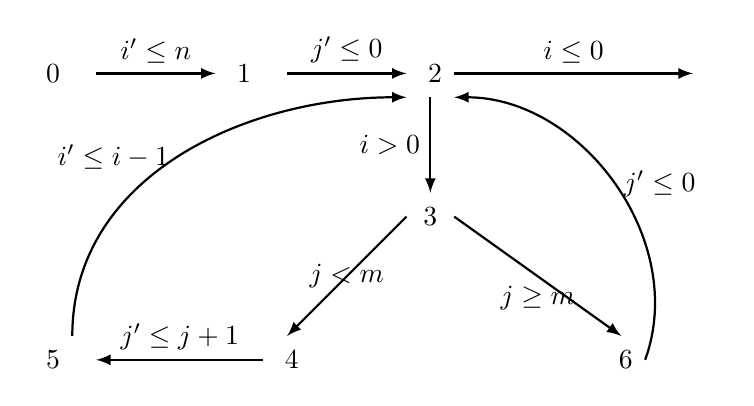
\begin{tikzpicture}[scale=\textwidth/20cm,samples=200]
  \draw[] (-8, 10) circle (0pt) node{{ $0$}};
  \draw[] (-4, 10) circle (0pt) node{{ $1$}};
  \draw[] (0, 10) circle (0pt) node{{ $2$}};
  \draw[] (0, 7) circle (0pt) node{{$3$}};
  \draw[] (-3, 4) circle (0pt) node{{ $4$}};
  \draw[] (-8, 4) circle (0pt) node{{ $5$}};
  \draw[] (4, 4) circle (0pt) node{{ $6$}};
  % Counter Variables
  \draw[] (6, 10) circle (0pt) node {\textbf{$\lex$}};
  %
  % Control Flow Edges:
  \draw[ thick, -latex] (-7, 10)  -- node [above] {$i' \leq n$}(-4.5, 10);
  \draw[ thick, -latex] (-3, 10)  -- node [above] {$j' \leq 0$}(-0.5, 10);
  \draw[ thick, -latex] (0, 9.5)  -- node [left] {$i > 0$} (0, 7.5) ;
  \draw[ thick, -latex] (0.5, 7)  -- node [below] {$ j \geq m $}  (4, 4.5);
  \draw[ thick, -latex] (-7.5, 4.5)  to  [out=90,in=180]  node [left] {$i' \leq i - 1$ }(-0.5, 9.5);
  \draw[ thick, -latex] (4.5, 4)  to  [out=70,in=0]   node [right] {$j' \leq 0 $}(0.5, 9.5);
  \draw[ thick, -latex]  (-0.5, 7) -- node  {$j < m$}  (-3, 4.5) ;
  \draw[ thick, -latex]  (-3.5, 4) -- node [above] {$j' \leq j + 1$}  (-7, 4) ;
  \draw[ thick, -latex] (0.5, 10)  -- node [above] {$i \leq 0$}  (5.5, 10);
  \end{tikzpicture}
  \caption{}
    \end{centering}
    \end{subfigure}
  \caption{
  (a) The Two Paths While Loop Example
    (b) The Abstract Execution Control Flow Graph}
      \label{fig:twoPathsWhile_abscfg}
  \end{figure}
  }
The program in Figure~\ref{fig:twoPathsWhile_abscfg}(a) is an example of two paths loop with different reachability-bounds on the control
locations in different paths.
Its abstract control flow graph is shown in Figure~\ref{fig:twoPathsWhile_abscfg}(b).
The edge $(0 \xrightarrow{i' \leq n} 1)$ on the top tells us the command 
$\clabel{\assign{i}{n}}^0$ is executed with a continuation point $1$, and the
command $\clabel{\assign{j}{0}}^1$ will be executed next.
The annotation $i' \leq 0$ is a difference constraint 
computed by $\absexpr$ over
the expression $n$ in the assignment command $\assign{i}{n}$.
It represents that the value of $i$ is less than or equal to value of $n$ after the
execution of $\clabel{\assign{i}{n}}^0$ and before executing $\clabel{\assign{j}{0}}^1$.
Another example constraint $i' \leq i - 1$ on the edge $5 \xrightarrow{i' \leq i - 1} 2$
describes the execution of
 the command at line $5$, 
$\clabel{\assign{i}{i - 1}}^{5}$. 
The $i'$ on the left side of $i' \leq i - 1$ represents the value of $i$ after the assignment operation,
and the right-hand side $i$ stores the value before the assignment.
The boolean constraint $i \leq 0 $ on the edge $2 \xrightarrow{i \leq 0} \lex$, 
represents the negation of the testing guard $i > 0$
in the $\ewhile$ command with loop header at line $2$.
$2 \xrightarrow{i \leq 0} \lex$ denotes that $i \leq 0$ must hold in order to perform this transition from program point $2$ to
the program exit. 
\end{example}
\section{Loop Refinement}
\label{sec:refine}
Three steps:
\begin{enumerate}
  \item It first collects all \emph{simple transition paths}.
  Every \emph{simple transition paths}, $\tpath \in \paths(\absG(c))$ 
  contains only the edges of atomic assignment or guard transitions without interleaving other paths.
  Each of them corresponds to a path in the flatten program in Definition~4.1 in \cite{GulwaniJK09}.
%
    \item \textbf{Rewrite the Program}
    Then it rewrites the program $c$ by rearranging all \emph{simple transition paths} as the syntax in \cite{GulwaniJK09} and preserves the same semantics.
\item \textbf{Refined Program}
Then it computes the 
refined program, $\rprog$ by Algorithm~1 in paper~\cite{GulwaniJK09}.
\\
This step invokes the algorithm REFINE from paper~\cite{GulwaniJK09} and compute the 
refined program $\rprog$ for a program $c$ given the rewritten program as input.
\end{enumerate}

\subsection{Collecting The Simple Transition Path}
We first collect the loop headers $\loopl(c) \subseteq \lvar(c)$ from a program $c$, which is the set of all program points corresponding to the loop headers in program $c$.
\begin{defn}[Loop Headers ($\loopl : \cdom \to \mathcal{P}(\ldom)$)]
  \label{def:loopl}
  \[
  \loopl(c) \triangleq 
  \left\{
    \begin{array}{ll}
      \{\}  & {c} = [{\assign x e}]^{l} \\
      \loopl({c_1}) \cup \loopl({{c_2}})  & {c} = {c_1};{c_2} \\
      \loopl(c_1) \cup \loopl({{c_2}})   & {c} =\eif([\bexpr]^{l}, c_1, c_2) \\
  \loopl(c') \cup \{l\}, &  {c}   = \ewhile ([\bexpr]^{l}, {c}')
  \end{array}
\right.
\]
  \end{defn}
% \begin{defn}[Loop Path]
%   \label{def:looppath}
% A simple transition path
% $\tpath \in \paths(\absG(c))$ for the program $c$, is a path on its abstract transition graph $\absG(c) = (\absV(c), \absE(c))$ with 
% \begin{itemize}
% \item a vertices sequence $(l_0, \ldots, l_n)$, where $l_i \in \absV(c)$ for every $i = 0, \ldots, n$ and
% %
% \item an edge sequence $(e_1, \ldots, e_n)$, where $e_i = (l_{i - 1}, dc_i, l_{i}) \in \absE(c)$ for every $i = 1, \ldots, n$,
% \end{itemize}
% %
% satisfying:
% \begin{itemize}
%   \item $l_i \neq l_j$ for every $i = 0, \ldots, n$ and $j = 0, \ldots, {n - 1}$,
%   \item $l_0$ is either the program point of a loop header or the program entrance ($l_0 = 0$),
%   i.e., $l_0 \in \loopl(c) \cup \{ 0 \}$
%   \item and $l_n$ is either the program point of a loop header or the program exit ($l_n = \lex$),
%   i.e., $l_0 \in \loopl(c) \cup \{ \lex \}$.
% \end{itemize}
% \end{defn}

\begin{defn}[Simple Tansition Path]
  \label{def:tpath}
A \emph{simple transition path}
$\tpath \in \paths(\absG(c))$ for the program $c$, is either a simple cyclic path, which has the same start- and end-point
or a simple path has either different while loop headers, the program entrance or exit as its start- and end-point
without visiting any loop header inside the path.
\\
Specifically, a path $l_0 \xrightarrow{dc_0} l_1 \xrightarrow{dc_1} \ldots l_n \in \paths(\absG(c))$ with the
vertices sequence $(l_0, \ldots, l_n)$, where $l_i \in \absV(c)$ for every $i = 0, \ldots, n$ and
%
the edge sequence $(e_1, \ldots, e_n)$, where $e_i = (l_{i - 1}, dc_i, l_{i}) \in \absE(c)$ for every $i = 1, \ldots, n$,
%
is a \emph{simple transition path} if and only if it satisfies,
\begin{itemize}
  \item $l_i \neq l_j$ for every $i = 0, \ldots, n$ and $j = 0, \ldots, {n - 1}$,
  \item $l_0$ is either the program point of a loop header or the program entrance ($l_0 = 0$),
  i.e., $l_0 \in \loopl(c) \cup \{ 0 \}$
  \item and $l_n$ is either the program point of a loop header or the program exit ($l_n = \lex$),
  i.e., $l_0 \in \loopl(c) \cup \{ \lex \}$,
  \item and $l_i \notin \loopl(c) \cup \{ 0, \lex \}$ for every $i = 1, \ldots, n-1$.
\end{itemize}
\end{defn}

\paragraph{Example.}
$2 \to 3 \to 6 \to 2$ is a transition path on $\absG(\kw{twoPathsWhile}(n, m))$ in Figure~\ref{fig:twoPathsWhile_abscfg}(b).
However, $2 \to 3 \to 6 \to 2 \to 3 \to 4 \to 5 \to 2$ is not a transition path because it is not simple (the program points $2$ and $3$ are visited twice).
In Figure~\ref{fig:threeWhile-overview}(b), $1 \to 2 \to 3 \to 4 \to 5 \to 6$ is not a transition path on $\absG(\kw{threeNestedWhile}(n, m, N))$ because it visits a loop header $3$ inside the path.

\subsection{Rewrite and Refine the Program}
\paragraph{Rewrite the Program}
\begin{algorithm}
  \caption{Program Rewriting $\kw{Rewrite}$}
  \label{alg:alg-refine_rewrite}
  \begin{algorithmic}[1]
    \REQUIRE program $c$
    \STATE finds all $c$'s \emph{simple transition path}s, $\tpath_1, \ldots, \tpath_n \in \paths(\absG(c))$.
    \STATE \textbf{init}: candidate set $W = \{c_1, \ldots, c_n\}$, where $c_i = \tpath_i$ and $i = 1, \ldots, n$
    \STATE \textbf{while} $W.size()> 1$:
    \STATE \quad create $c' = \rpchoose{c_1, \ldots, c_m}$ 
    s.t. $c_i \in W \land c_i[0] = c_j[0] \land c_i[-1] = c_j[-1], i, j = 1, \ldots, m$.
    \\ \quad $W.add(c')$ \qquad $W.remove(c_1, \ldots, c_m)$
    \STATE
    \quad create $c' = \rprepeat(c)$ s.t. $c_i \in W \land c[0] = c[-1] \land c[0] \in \loopl(c)$
    \\ \quad $W.add(c')$, \qquad $W.remove(c)$
    \STATE \quad create $c' = c_1; c_2$ s.t. $c_1, c_2 \in W \land c_1[-1] = c_2[0]$
    \\
    \quad $W.add(c')$ \qquad $W.remove(c_1, c_2)$
    \STATE \textbf{Endwhile}
    \\ $c^T = W[0]$
    \RETURN $c^T$.
\end{algorithmic}
\end{algorithm}
%
Line-2: initialize each candidate $c_i$ with a simple transition path $\tpath_i$.
\\
Line-4: for all the candidates $c_1, \ldots, c_m$ having the same starting and ending vertices, rewrite them into if statement as~\cite{GulwaniJK09}.
\\
Line-5: for every candidate $c'$, if it starts and ends with the same vertex, rewrite it into while loop statement as~\cite{GulwaniJK09}.
\\
Line-6: for every two candidates $c_1, c_2$, if $c_1$ ends with the same vertex as $c_2$'s starting label, rewrite them into sequence statement as~\cite{GulwaniJK09}.
\\
We use simple depth first search strategy computes all the \emph{simple transition path}s satisfying the Definition~\ref{def:tpath} below.
It guarantees that  every $\tpath$ is equivalent to a path $\rho$ in Definition~4.1 of \cite{GulwaniJK09}.

\paragraph{Refined Program}
We implement the algorithm REFINE from paper~\cite{GulwaniJK09} and compute the 
refined program $\rprog$ for a rewritten program $c$.

\section{Ranking Function Computation and Estimation}
\label{sec:rank}
Three steps:
\begin{enumerate}
    \item It first collects three edge sets for each variable,
  in which the variable increases, decreases and reset respectively.
  \item
  Then, it assigns a symbol $x \in \scvardom$ to the edge on which this symbol decreases as this edge's ranking function.
  \item
  In the last step, it estimates the upper bound invariant on the maximum value of each ranking function recursively.
  In the meantime, it also computes a loop bound path-insensitivity for each loop, which can be used to compute the path reachability-bound later.
  \end{enumerate}

  The algorithm in this step is inspired from the Algorithm.2 in paper~\cite{SinnZV14},
  % which assigns a variable to each edge on which this variable decrease as its ranking function.
  the Algorithm.3 in paper~\cite{ZulegerGSV11},
  and the Definition.25 in Section 4 of paper~\cite{SinnZV17}.
  Algorithm.3 in paper~\cite{ZulegerGSV11} assigns a set of variables to each transition in which these variables decrease as the local bound
  and estimates the maximum value each variable in this set.
  Algorithm.2 in paper~\cite{SinnZV14} assigns a variable to each edge on which this variable decrease as its ranking function
  and then estimates the maximum value for the ranking function.
  The Definition.25 in paper~\cite{SinnZV17}
  assigns each transition with a variable that decreases in this transition, as the local bound and computes the bound similarly.
  %
  \subsection{Collecting Variable Modifications}
  For each variable $x$ in a program $c$, this step computes three edge sets, $\inc(x, c)$, $\dec(x, c)$,
  and $\reset(x, c)$ for $x$.
  Every edge in a set corresponds to a transition in which $x$ is increased,
  %  $\inc(x, c)$,
  decreased
  % $\dec(x, c)$ and 
  or reset
  % $\reset(x, c)$, 
  respectively.
  \\
  $\inc: \cdom \to \vardom \to \mathcal{P}(\absevent) $
  is the set of the edges where the variable increase, 
  %\\
  \[ \inc(x, c) = \left\{ \absevent | \absevent = (l, x' \leq x + v, l') \land \absevent \in \absflow(c) \right\} \]
  %\\
  $\dec: \vardom \to \mathcal{P}(\absevent) $
  is the set of abstract events where the variable decrease,
  %\\
  \[\dec(x, c) = \left\{\absevent| \absevent = (l,  x' \leq x - v, l') \land \absevent \in \absflow(c) \right\}\]
  %\\
  $\reset: \cdom \to \vardom \to \mathcal{P}(\absevent) $ is the set of the abstract events where the variable is reset,
%
  \[\reset(x, c) = \left\{ \absevent| \absevent = (l,  x' \leq y - v, l') \land x \neq y \land \absevent \in \absflow(c) \right\}\]
  Additionally,
  we also compute the reset graph $\resetG(c)$ and the reset chain, $\resetchain(x, c) \in \mathcal{P}(\mathcal{P}(\absevent))$ for every rank $x$.
  The $\resetchain(x, c)$ for every rank $x$ contains all the paths in $\resetG(c)$ that are end at $x$.
  The computation of $\resetG(c)$ and $\resetchain(x, c)$ follows the Definition~20 in~\cite{SinnZV17}.
  \[\resetG(c) = (\resetV(c), \resetE(c))\]
  \[\resetE(c) = \left\{ (x, \absevent, y) ~\vert~ \absevent \in \reset(x, c) \land \absevent = (l, x' \leq y + c, l') \right\} \]
  \[\resetV(c) = \left\{ x ~\vert~ (x, \_, \_) \in \resetE(c) \lor (\_, \_, x) \in \resetE(c) \right\} \]
  In a variable $x$'s reset chain set, $\resetchain(x, c)$, in each chain $(e_0, \ldots, e_m) \in \resetchain(x, c)$
  a variable $x_i$ is reset by another variable $x_{i + 1}$ on edge $e_{i}$
  and $x_{i + 1}$ is reset on edge $e_{i + 1}$ recursively
  for every $i = 0, \ldots, m - 1$.
  $x$ is reset on the first edge $e_0$ of every sequence in $\resetchain(x, c)$.
  {Each edge $e_i$ in a sequence $(e_0, \ldots, e_m) \in \resetchain(x, c)$
  resets a variable $x_i$ by another variable $x_{i + 1}$ such that $x_{i + 1}$
  is reset on edge $e_{i + 1}$ recursively. The first edge $e_0$ of each sequence resets the variable $x$.}
  % 
  \\
  In the following steps, $c$ is omitted in $\inc(x, c)$,
  $\dec(x, c)$ and $\reset(x, c)$ for concise when the reference of a program $c$ is clear in the context.

  \subsection{Assigning The Ranking Function to An Edge}
  For each edge in the transition graph $\absG(c)$ of a program $c$,
  this step assigns the variable that decreases on this edge as the ranking function of this edge.
  This step adopts the local bound computation method in Section 4 of~\cite{SinnZV17} to assign the local bound to each edge,
  formally as follows.
  \begin{defn}[Ranking Function Generatation]
  \label{def:ranking_gen}
  For every edge $\absevent$ in the transition graph $\absG(c)$ of a program $c$,
  its \emph{ranking function/local bound}, $\locbound(\absevent, c)$
  is the variable that decreases on this edge, computed as follows,
  %
  \[ 
\begin{array}{ll}
  \locbound(\absevent, c) \triangleq 1 
  & \absevent \notin SCC(\absG(c))
  \\
  \locbound(\absevent, c) \triangleq x
  & \absevent \in SCC(\absG(c)) \land \absevent \in \dec(x, c) \land  \absevent = (\_, \_ , x' \leq x - v) \\
  \locbound(\absevent, c) \triangleq x
  & \exists \absevent' \in \absG(c), \tpath \in \paths( \absG(c)) \st \absevent, \absevent' \in \tpath \land \locbound(\absevent', c) = x \\
  % \in SCC(\absG(c)) \land \absevent \in \dec(x, c) \land  \absevent = (\_, \_ , x' \leq x - v) \\
  \locbound(\absevent, c) \triangleq x
  & \absevent \in SCC(\absG(c)) \land 
  \absevent  \notin \bigcup_{x \in \vardom} \dec(x, c)
  \land \absevent \notin SCC(\absG(c) \setminus \dec(x, c))\\
  \locbound(\absevent, c) \triangleq \infty
  & o.w..
\end{array}
\]
  $SCC(\absG(c))$ is the set of all the strong connected components of $\absG(c)$.
  \end{defn}
    The first case is straightforward. 
    For the label $l$ which is not in any while loop, 
    the labeled command with the label $l$ will be 
    evaluated at most once. 
    The second and third cases are guaranteed by the \emph{Discussion on Soundness} in Section 4 in~\cite{SinnZV17}.
    The soundness is formalized in Lemma~\ref{lem:local_bound_sound} with proof in Appendix~\ref{apdx:pathinsensitive_rb_soundness}.
  %
  \paragraph{Example}
  In Figure~\ref{fig:relatedNestedWhileOdd-overview}(b), we assign variable $i$ to edge $7 \xrightarrow{i' \leq i - 1} 1$ as ranking.
  If we remove this edge, the edges on $\tpath_2$ and $\tpath_1$ are not in any SCC, so they also have the same ranking.
In the same way, ranking for edges on $\tpath_4$ is $i$ as well and $k$ for them on $\tpath_3$.


  \subsection{Ranking Function Estimation}
  This step estimates the upper bound, $\varinvar(x, c) \in \scexpr(c)$
  on the maximum value for each ranking function  $x \in  \vardom \cup \scvar(c)$.
  \\
  For a program $c$, the \emph{ranking function bound},
  $\varinvar(\locbound(\absevent, c), c)$ is 
  the bound on the maximum value of the ranking function  
  assigned to the edge $\absevent \in \absE(c)$, formally in Definition~\ref{def:ranking_bound}.
  \\
  In order to estimate the maximum value of $\locbound(\absevent, c)$ assigned to edge $\absevent \in \absE(c)$,
  the bound on the iteration times of each corresponding edge, $\absclr(\absevent, c)$ 
  is computed interactively in a path-insensitive manner.
  % \\ 
  % $\varinvar (x, c) \in \scexpr(c)$
  % \\
  % $\absclr(\absevent, c) \in \scexpr(c)$
  \begin{defn}[Ranking Function Estimation]
    \label{def:ranking_bound}
  For a program $c$ and an edge $\absevent \in \absE(c)$,
  the \emph{ranking function bound}, 
  $\varinvar(\locbound(\absevent, c), c)$ for the ranking function $x = \locbound(\absevent, c)$
  of this edge
  is computed as follows,
    \[ 
  \begin{array}{lll}
    \varinvar(x, c) & \triangleq x & x \in \scvar(c) \\
    \varinvar(x, c) & \triangleq \incrs(x, c) + \max\left\{\varinvar(y, c) + v ~\mid~ (l, x' \leq y + v, l') \in \reset(x, c) \right\} & x \notin \scvar(c)
  \end{array}
  \]
  %
  where $\incrs(x, c) \triangleq \sum\limits_{\absevent \in \inc(x, c)}\{\absclr(\absevent, c) \times v ~\mid~ \absevent = (l, x' \leq x + v, l')\}$
  The path-insensitive bound, $\absclr(\absevent, c) \in \scexpr(c)$  on the execution times of the transition $\absevent$, is interactively computed as well as below,
\[ 
\begin{array}{lll}
  \absclr(\absevent, c) 
  & \triangleq \varinvar(\locbound(\absevent, c), c)  &  \\
  & \quad \text{if} ~ \locbound(\absevent, c) \in \scvar(c) & \\
  \absclr(\absevent, c) 
  & \triangleq
    \sum \left\{ \incrs(y, c) | ch \in \resetchain(x, c) \land y \in ch \right\} & \\
    & \quad + 
  \sum\limits_{ch \in \resetchain(x, c)}
  \min \left\{\absclr(\absevent', c) ~\mid~ \absevent' \in ch\right\} \times 
  \big(\varinvar(in(ch), c) 
  + \sum\limits_{(\_, (\_, x' \leq y + v, \_), \_) \in ch} v \big) & \\
  &  \quad \text{if} ~\locbound(\absevent, c) = x \land x \notin \scvar(c) & ,
\end{array}
  \]
 where $in(ch)$ is the first vertex of the reset chain $ch$.
\end{defn}
  %
We also have the soundness of this path-insensitive transition bound. For a program $c$ and an edge $\absevent \in \absE(c)$,
$\absclr(\absevent)$ is a sound upper bound
on the execution times of this transition by paper~\cite{SinnZV17}, formally below in Theorem~\ref{thm:pathinsensitive_rb_soundness} with proof in Appendix~\ref{apdx:pathinsensitive_rb_soundness}.
%
\begin{thm}[Soundness of the Path-insensitive Transition Bound]
  \label{thm:pathinsensitive_rb_soundness}
For each program ${c}$ and an edge $\absevent = (l, \_, \_) \in \absG(c)$, if $l$ is the label of an assignment command,
%  label $l \in \lvar(c)$,
then its \emph{path-insensitive transition bound} $\absclr(\absevent, c)$ 
 is a sound upper bound on 
the execution times of this assignment command in $c$.
  \[
    \begin{array}{l}
      \forall \trace_0 \in \ftdom_0(c), \trace \in \tdom, c \in \cdom, l, l' \in \lvar(c) \st
      \Big( \config{c, \trace_0} \rightarrow^{*} \config{\clabel{\eskip}^{l'}, \trace_0 \tracecat \trace} 
        \lor  \config{c, \trace_0} \uparrow^{\infty} \trace_0 \tracecat \trace \Big)
       \\ \qquad \qquad
       \implies
       \exists \absevent = (\_, l, \_) \in \absflow(c) \land
      \counter(\trace, l) \leq \econfig{\absclr(\absevent, c)}(\trace_0)
    \end{array}
  \]
\end{thm}
%
\paragraph[example]{Example.}
% \todo{The w example}
Using this ranking function based approach, we first find the ranks for every transition,
$\locbound(0 \to 1) = 1$,
$\locbound(1 \to \lex) = 1$,
$\locbound(1 \to 2) = i$,
$\locbound(2 \to 3) = i$,
$\locbound(3 \to 4) = i$,
$\locbound(4 \to 5) = k$,
$\locbound(5 \to 4) = k$,
$\locbound(4\to 6) = \locbound(6 \to 7) = \locbound(7 \to 1) = i$,
and $\locbound(2 \to 8) = \locbound(8 \to 1) = i$,
Then we estimate the upper bound invariant for the ranking function $i$ and $k$ by computing the transition bound in the same time.
We get $\varinvar(i, c) = n$ and $\varinvar(k, c) = m$.
While the transition bound for each transition is the same as the upper bound invariant of its ranking function.
They are loose and path-insensitive. 

Specifically, in Example~\ref{ex:relatedNestedWhileOdd-overview}, the ranking $i$ is reset by $n$ at edge $0 \to 1$ and 
$k + m$ at edge $6 \to 7$ and $k$ is assigned value $i - m$ at edge $3 \to 4$. Through reset chain graph (which we do not fully presented but can be found in the Definition~20 in~\cite{SinnZV17}), we estimate a symbolic value $n$ for both ranking variable $i$ and $k$.
Interactively, iteration bounds for all the edges in this loop are $n$ as well path-insensitively.
\section{Path-sensitive Reachability-bound Algorithm}
\label{sec:psrb}
Our path-sensitive reachability-bound algorithm relies on the \emph{Abstract Transition Graph}, $\absG(c)$, the \emph{Refined Program}, $\rprog$ and the upper bound invariant of the \emph{Ranking Function} computed previously for the program $c$.
It first requires to compute the new quantities, \emph{Path Reachability-bound} and the \emph{Loop Reachability-bound}, and this section introduces the definition and the following sections describe how we compute them.
%  of \emph{Path Reachability-bound} and the \emph{Loop Reachability-bound}. 

% Given a program $c$ with its \emph{Abstract Transition Graph}, $\absG(c)$ and refined program $\rprog$, our path-sensitive reachability-bound algorithm is presented as follows.

As pre-procedures, we first need to compute the loop bound, $BD(\rprog', c) \in \scexpr(c)$ for every subprogram $\rprog'$ of $c$ in $\rprog$, and use it to estimate the \emph{path local reachability-bound}, $\outinB(\rprog_l, \tpath, c) \in \scexpr(c)$ for each $\tpath$ w.r.t. the sub loop program $\rprog_l$.
\begin{defn}[Loop Bound]
  % \label{def:loopbound}
  For any program $c$ with it refined program $\rprog$,
  the loop bound $BD(\rprog', c) \in \scexpr(c)$ for a subprogram $\rprog'$ of $c$ in $\rprog$ is a upper bound on the iterating times of this program from its enter point to the exit point.
\end{defn}
% 
% Then we compute the \emph{path local reachability-bound}, $\outinB(\rprog_l, \tpath, c) \in \scexpr(c)$ for every sub loop program $\rprog_l$ of $c$ in $\rprog$.
\begin{defn}[Path Local Reachability-bound]
  % \label{def:pathlocalrb}
  Given program $c$ with its refined program $\rprog$ and a simple transition path $\tpath$ in this program, 
  let $l: \rprog_l = \kw{enclosed}(\rprog, \tpath)$ be a sub loop program in $\rprog$,
  then $\tpath$'s \emph{path local reachability-bound} w.r.t. $l: \rprog_l$,  $\outinB(\rprog_l, \tpath, c) \in \scexpr(c)$
  is an upper bound on the execution times of $\tpath$ when executing program $\rprog$.
\end{defn}
Intuitively,
% the local reachability-bound of a \emph{simple transition path},
$\outinB(\rprog_l, \tpath, c)$ bounds the execution times of $\tpath$ when executing its innermost loop program $\rprog_l$.
% and $\rprog$ is the closest loop where $\tpath$ is nested.
For example in the first interleaving pattern $\rprog_1^1$ in Example~\ref{ex:relatedNestedWhileOdd-overview}, 
$4:\rprepeat(\tpath_3)$ is the innermost loop program of $\tpath_3$. So we first compute $m - n$ as its \emph{path local reachability-bound} to bound its iteration times in its closest loop by Section~\ref{sec:pathlocalrb}.
% $4:\rprepeat(\tpath_3)$ is the innermost loop program of $\tpath_1$, $\tpath_2$ and $\tpath_4$.
% We compute the $\frac{m}{4}$ for all the three path $\tpath_1$, $\tpath_2$ and $\tpath_4$ w.r.t. $\rprog_1^1$, as their \emph{path local reachability-bound}.
% $\outinB(1: \rprog_1^1, \tpath_1) = \frac{m}{4}$,
% $\outinB(1: \rprog_1^1, \tpath_2) = \frac{m}{4}$,
% $\outinB(1: \rprog_1^1, \tpath_4) = \frac{m}{4}$,

Next, we define the \emph{loop reachability-bound},
$\lpchB(l: \rprog_l, \tpath, c) \in \scexpr(c)$ for every outer loop program $\rprog_l$ of $\tpath$ in $\rprog$. This quantity aims to precisely bound the iteration numbers of the outer loop $l$,
such that,
during these iterations, the innermost loop $l' = \kw{enclosed(\tpath)}$ is executed, i.e., reached.
\begin{defn}[Loop Reachability-bound]
% \label{def:looprb}
For a program with its refined program $\rprog$ and a simple transition path $\tpath$ in this program, 
let $l: \rprog_l$ be a loop program in $\rprog$,
then $l: \rprog_l$'s \emph{loop reachability-bound} w.r.t. $\tpath$,  $\lpchB(l: \rprog_l, \tpath, c) \in \scexpr(c)$
is the upper bound on iteration numbers of the outside loop $l$,
such that,
during these iterations, the nested loop $l' = \kw{enclosed(\tpath)}$ is entered.
\end{defn}
As introduced in Section~\ref{sec:overview} for Example~\ref{ex:relatedNestedWhileOdd-overview}, $\tpath_3$ has an outer loop program $\rprog_1^1$. Since $L_4$ will be ``entered'' only in the first iteration of $\rprog_1^1$,
we aim to compute $1$ for $\lpchB(\rprog_1^1, \tpath_3, c)$ in Section~\ref{sec:looprb}.
  % and we compute $\lpchB(\rprog_1^1, \tpath_3, c) = 1$. It is tight because the innermost loop of $\tpath_3$ will be ``entered'' only in the first iteration of $\rprog_1^1$.

% Intuitively $\lpchB(l: \rprog_l, \tpath, c) \in \scexpr(c)$
% is the bound on iteration numbers of the outside loop $l$,
% such that,
% during these iterations, the nested loop $l' = \kw{enclosed(\tpath)}$ is executed, i.e., reached.
The \emph{path reachability-bound}, $\inoutB(\rprog, \tpath)$ for each $\tpath$
aims to bound the execution times of $\tpath$ globally during the execution of $c$ and Section~\ref{sec:pathrb} presents the estimating algorithm.
%
\begin{defn}[Path Reachability-bound]
% \label{def:pathrb}
For a program $c$ with its refined program $\rprog$ and a simple transition path $\tpath$ in this program, 
$\tpath$'s reachability-bound, $\inoutB(\rprog, \tpath) \in \scexpr(c)$ is the upper bound on the
execution times of $\tpath$ when executing the $\rprog$.
\end{defn}
% Intuitively, $\inoutB(\rprog, \tpath)$ bounds the execution times of $\tpath$ globally during the execution of $c$.

For our running program in Example~\ref{ex:relatedNestedWhileOdd-overview}, since there isn't nested loop for $\tpath_1, \tpath_2$ and $\tpath_3$, we compute their $\inoutB(\rprog, \tpath) = \frac{m}{4} $, which is the same as their local bound.
While for $\tpath_3$ we compute  the $\inoutB(\rprog, \tpath_3) = \frac{m}{4} \times 1$ by multiplying its local bound with loop reachability bound.
% path is $\tpath_3 = \frac{m}{4} \times 1 = \frac{m}{4} $.

% \paragraph{Program Points Reachability-bound Computation}
% \label{sec:point-psrb}
The \emph{Reachability-bound} for program points is finally computed as follows.
For each program point in a program $c$, $l \in \lvar(c)$,
%  in a program $c$,
its \emph{reachability-bound}, $\psRB(c, l)$ during the execution of $c$ is computed as follows.
%
\begin{defn}[Program Point Reachability-bound Computation]
\label{def:point_psrb}
Given a program $c$ with its \emph{Abstract Transition Graph}, $\absG(c)$ and refined program $\rprog$,
the \emph{reachability bound} of each program point $l \in \lvar(c)$, $\psRB(c, l)$ 
sums up all the path reachability bounds, $\inoutB(\rprog, \tpath)$ over all simple transition paths $\tpath$ that contains the program point $l$.
\[ 
  \psRB(c, l) = 
  \sum
  \left\{ \inoutB(\rprog, \tpath) ~\vert~ \tpath \in \rprog \land 
  l \in \tpath \right\}\footnotemark
\]
$l \in \tpath$ denotes that the program point $l$ is a vertex on $\tpath$ 
and $\tpath \in \rprog$ denotes $\tpath$ is a simple transition path in $\absG(c)$.
\footnotetext{$l \in \tpath$ and $\tpath \in \rprog$, the $\in$ notation is abused to denote
the program point $l$ is a vertex on this path and $\tpath$ is a simple transition path on $\absG(c)$ respectively.}
\end{defn}
$\econfig{\psRB(c, l)}$ is a \emph{reachability-bound} for every program point $l$ in a program $c$.
\begin{thm}[Soundness of the Path-sensitive Reachability-bound Estimation]
\label{thm:pathsensitive_rb_soundness}
For every program ${c}$ and every label $l$ in this program,
$\econfig{\psRB(c, l)}$ is a \emph{Reachability-bound} for $l$ in $c$.
%
{\small
\[
  \begin{array}{l}
    \forall c, c_r \in \cdom, \tpath \in \absG(c), \trace_0 \in \ftdom_0(c),  \trace_r \in \ftdom_0(c_r), \trace \in \tdom, l, l' \in \ldom, \rprog \st 
    \\ \qquad
    \rprog = REFINE(\algrewrite(c))
    \land 
    \rprog = \algrewrite(c_r)
    \land
    \\ \qquad
    \land
    \Big(
    \config{c_r, \trace_0} \rightarrow^* \config{\clabel{\eskip}^{l'}, \trace_0 \tracecat \trace}
    \lor \config{c_r, \trace_0} \uparrow^{\infty} \trace_0 \tracecat \trace 
    \Big)
    \\ \qquad
    \implies \econfig{\psRB(c, l)}(\trace_0) \geq \counter(\trace, l)
  \end{array}.
\]
}
\end{thm}
\section{Path Local Reachability-bound Computation}
\label{sec:pathlocalrb}

\subsection{Loop Bound Computation}
There are three methods for computing the loop bound, $BD(\rprepeat(\rprog'), c)$ for every sub program, specifically loop program $\rprepeat(\rprog')$ in a program $c$'s refined program $\rprog$:
\begin{enumerate}
  \item Estimated by $BD(\rprepeat(\rprog'), c) = BOUND(\rprepeat(\rprog'))$ from paper~\cite{GulwaniJK09}, which is precise for simple loop without nested loops but not for nested loops. We are not giving the computation detail in this paper, which can be found in paper~\cite{GulwaniJK09}.
  \item Estimated by Equation~\ref{eq:absBD} in Section~\ref{sec:loopbound-rankbased} path-insensitively based on the estimated ranking function from Section~\ref{sec:rank}. This bound is precise when there is only one path in this loop but not for loops with multiple paths.
  \item   We provide an alternative computation method using the variable invariant estimation idea from~\cite{SinnZV17} in Definition~\ref{def:loopbound} and the progress invariant idea from~\cite{GulwaniJK09}.
  We compute the rank functions' abstract states, $\rfinit(\rprog, c)$, $\rffinal(\rprog, c)$, $\rfnext(\rprog, c)$ and $\varGD(\rprog, c)$ as in Definition~\ref{def:alg-absstate}.
  Then we compute $BD(\rprepeat(\rprog'), c)$ by Definition~\ref{def:loopbound} using SMT solver.
\end{enumerate}
%
\subsubsection{Ranking Function Based Loop Bound Computation}
\label{sec:loopbound-rankbased}
Based on the estimated ranking function from Section~\ref{sec:rank}, the $BD(\rprog, c)$ for the refined program $\rprog$ can be estimated by $\absclr(\absevent, c)$ by taking the
minimum value over all $\absevent \in \rprog$.
We use $\absevent \in \rprog$ to denote $\absevent$ is an edge on path $\rprog$.
\begin{equation}
  \label{eq:absBD}
  BD(\rprog, c) = \min\left\{ \absclr(\absevent, c) \middle\vert \absevent \in \rprog \right\}.
\end{equation}
%
This bound is accurate on the iteration numbers of a single loop, but neither tight on the iterations of different paths inside the loop, nor the nested loop.
%
\paragraph{Walk through Example.}
% \todo{The walk through example}
In Figure~\ref{fig:relatedNestedWhileOdd_abscfg}(b), by using this ranking function-based approach, we compute the loose loop bound for each subprogram,
$BD(\tpath_0) = 1$, $BD(\tpath_5) = 1$, $BD(\rprepeat(\tpath_3)) = n - m$, $BD(\rprog_1^1) = n$, and $BD(\rprog_1^2) = n $.
The bounds for $\rprog_1^1$ and $\rprog_1^2$ are both $n$ while expected to be $\frac{m}{4}$.
They are loose because of the nature of the path-insensitivity in the ranking function invariant computation in Definition~\ref{def:ranking_bound}. 

\subsubsection{New Approach of Computing The Loop Bound} 
Our new approach also uses the ranking function, but combines with the refined program.
We first compute the refined abstract states for ranking function in different program point and different local program based on the refined program.
Then we these precise abstract state, and estimate the loop bound path sensitively.

\begin{defn}[Rank Abstract States Computation]
  \label{def:alg-absstate}
  Given a program $c$, with $\rprog$ as a sub-program in $c$'s refined program, where $\rprog \subseteq REFINE(\kw{Rewrite(c)})$, let $c_r$ be the while program such that $\rprog = \algrewrite(c_r)$,
  we compute four different abstract states for the ranking functions of this sub program, 
  $\rfinit(\rprog, c)$, $\rffinal(\rprog, c)$, $\rfnext(\rprog, c)$ and $\varGD(\rprog, c)$ as follows.
 \begin{itemize}
  \item We first compute the initial execution point and continuation execution points of $\rprog$ as
  $\absinit(\rprog) = \absinit(c_r)$
  and 
  $\absfinal(\rprog) = \absfinal(c_r)$ where $\rprog = \algrewrite(c_r)$.
  \item The \emph{Initial State}, 
  $\rfinit(\rprog, c)$ is a set of equations $x = e$, where $e \in \scexpr(c)$ is a
  symbolic expression describing the initial value of $x$ before executing $\rprog$.
  Each $x$ is the ranking function of a simple transition path $\tpath$ in this program. 
  It contains the initial value for every ranking function of the simple transition path $\tpath$ in this program.
 \[
   \rfinit(\rprog, c) \triangleq 
   \bigcup_{x \in \left\{ \locbound(\absevent, c) | \tpath \in \rprog \land \absevent \in \tpath \right\} }
   \left \{ 
   x = \arg\max_{l_1}\left\{
     \varinvar(y, c) + v ~\middle\vert~ 
     \begin{array}{l} 
       (l_1, x' \leq y + v, l_2) \in \reset(x, c) 
       \\
     \land l_1 \leq \absinit(\rprog, c)
   \end{array}
   \right\}
   \right\}
   \]
 $\rfinit(\tpath, c)$ can also be computed using the function $\kw{INIT(c, 0, \absinit(\rprog))}$ in \cite{GulwaniJK09}. 
 %
 \item  The \emph{Final State}, $\rffinal(\rprog, c)$ a conjunction of boolean expressions.
 It is the post-condition
 after the execution of $\rprog$.
 % \\
 \[
  \begin{array}{l} 
    \rffinal(\rprog, c) \triangleq 
    \\
   \bigcup\limits_{x \in \left\{ \locbound(\absevent, c) | \tpath \in \rprog \land \absevent \in \tpath \right\} }
   \left \{ 
   x = \min\limits_{ \left\{ l_1 ~|~ l_1 \geq \pi_2(\absfinal(\rprog, c)) \right\} }
   \max\left\{
     v ~\middle\vert~ 
     \left( (x = v) \land \bigwedge\limits_{b \in \kw{Guard}(\rprog, c)} \neg b \right) \neq \efalse
   \right\}
   \right\}
  \end{array}
  \]
  $\kw{Guard}(\rprog, c)$ is the set of all the unique boolean expressions (i.e., the boolean constraints) on this program.
 \item The \emph{Next State}, $\rfnext(\tpath, c) \in \scexpr(c)$ 
 is a
 symbolic expression describing how much $\tpath$'s ranking function ($\locbound(\tpath)$) is changed after the first execution of $\rprog$ and before the second execution.
 \[
   \begin{array}{l}
   \rfnext(\tpath, c) \triangleq 
   \\
   \bigcup\limits_{x \in \left\{ \locbound(\absevent, c) | \absevent \in \tpath \right\}}
   \left\{ x = \begin{array}{l}
  \sum\limits_{\absevent \in \inc(x, c) }
   \left\{ v ~\middle\vert~ \absevent = (l, x' \leq x + v, \_) \land l \in \tpath\right\}
   \\ \qquad 
   + \arg\max\limits_{l' }
      \left\{ \varinvar(y, c) + v ~\middle\vert~ (l, x' \leq y + v, l') \in \reset(x, c) \land l \in \tpath\right\}
      \\ \qquad 
     - \sum\limits_{ \absevent \in \dec(x, c) }\left\{ 
       v ~\middle\vert~ \absevent = (l, x' \leq x - v, \_) \land l \in \tpath 
       \right\}
     \end{array}
   \right\} 
   \end{array}
 \]
 Indeed we only compute the $\rfnext(\tpath)$ because that the recursion is exhausted into the base case, i.e. $\tpath$ when computing $\varGD(\rprog, c)$ as below.
 \item  The \emph{Variable Gradient Decent}, 
 $\varGD(\rprog, c)$
 is a set of equations $x = e$ for the same variables in the $\rfinit(\rprog, c)$.
 It computes the set of next states for every ranking function of the simple transition path $\tpath$ in $\rprog$,
 and recursively computes the loop bound, $BD(\rprog, c)$ in the meantime.
 \\
 {$\varGD(\rprepeat(\rprog), c) =  BD(\rprog, c)  \times
{\varGD(\rprog, c)}$}
 \\
 $\varGD(\rprog_1;\rprog_2, c) =  \varGD(\rprog_1, c) + \varGD(\rprog_2, c)$
 \\
 $\varGD(\tpath, c) =  \min\left\{v  ~|~ x = v \in \rfnext(\tpath, c) \right\}  $  
\end{itemize}
\end{defn}
The computation of the \emph{Variable Gradient Decent}, 
$\varGD(\rprog, c)$ involves the computation of $BD(\rprog, c)$ recursively as follows.
\begin{defn}[Loop Bound Computation]
\label{def:loopbound}
  \[
    \begin{array}{rcl}
      BD(\tpath, c) & \triangleq & 1 \\
      BD(\rprog_1;\rprog_2, c) & \triangleq & \min \left\{BD(\rprog_1, c), BD(\rprog_2, c) \right\} \\
      BD(\rpchoose{\rprog_1, \ldots, \rprog_m }, c) & \triangleq 
      & \max\left\{ BD(\rprog_1, c), \ldots, BD(\rprog_m, c) \right\} \\
      BD(\rprepeat(\rprog'), c) & \triangleq 
      &
      \max\limits_{x \in \left\{ \locbound(\absevent, c) | \tpath \in \rprog' \land \absevent \in \tpath \right\}}
      \Big\{ \highlight{\frac{a - b}{\varGD(\rprog', c)}} ~\vert~
      x = a \in \rfinit(\rprog', c)
      \\ & & \qquad \qquad \qquad \qquad \qquad \qquad \qquad 
      \land x = b \in \rffinal(\rprog', c)
      \Big\} 
      \\
      BD(l: \rprog_l, c) & \triangleq & BD(\rprog_l, c)
    \end{array}
  \]
\end{defn}
We show that Definition~\ref{def:loopbound} computes a sound loop bound for every loop in a refined program below in Lemma~\ref{lem:loopbound_sound} with proof in \highlight{Appendix~\ref{apdx:loopbound-sound}}.
\begin{lem}[Soundness of Loop Bound]
  \label{lem:loopbound_sound}
  For every program $c$ with it refined program $\rprog$,
  % for every loop $\rprepeat(\rprog')$ inside $\rprog$, 
  $BD(\rprog, c)$ is a sound upper bound on the iterating times of this program.
\end{lem}

\paragraph{Walk through Example.}
% \todo{The walk through example}
Using our new approach, we compute a more precise loop bound $BD(\rprog)$ for each subprogram of our walk through example in Figure~\ref{fig:relatedNestedWhileOdd_abscfg}(b), in comparison to the purely ranking function-based approach in Equation~\ref{eq:absBD}.
Specifically for $\rprog_1^1$ and $\rprog_1^2$, we compute $BD(\rprog_1^1) = \frac{m}{4}$ and $BD(\rprog_1^2) = \frac{m}{4}$ as expected,
and compute the same bounds for the other sub-programs.
% $BD(\tpath_0) = 1$, $BD(\tpath_5) = 1$, $BD(\rprepeat(\tpath_3)) = n - m$, $BD(\rprog_1^1) = n$, and $BD(\rprog_1^2) = n $.
% The bounds for $\rprog_1^1$ and $\rprog_1^2$ are both $n$ while expected to be $\frac{m}{4}$.
% They are loose because of the nature of the path-insensitivity in the ranking function invariant computation in Definition~\ref{def:ranking_bound}. 


\subsection{Path Local Reachability-bound}
We first compute $\kw{enclosed}(\rprog, \tpath)$, which is \textbf{the innermost loop} inside $\rprog$ where $\tpath$ is located. Then by using the loop bound computed by our new approach, we compute the \emph{path local reachability-bound} of
the $\tpath$ in its closest nested loop as follows in Definition~\ref{def:pathlocalrb}.
\begin{defn}[Path Local Reachability-bound Computation]
    \label{def:pathlocalrb}
    Given program $c$ with its refined program $\rprog$ and a simple transition path $\tpath$ in this program, 
    let $l: \rprog_l = \kw{enclosed}(\rprog, \tpath)$ be a sub loop program in $\rprog$,
    then $\tpath$'s \emph{local reachability-bound} $\outinB(\rprog_l, \tpath, c)$ w.r.t. $l: \rprog_l$
    is computed inductively as follows.
    The input $c$ is omitted in the following equations for concise given the context is clear.
  \[
    \begin{array}{rcl}
      \outinB(\tpath, \tpath) & \triangleq & 1 \\
      \outinB(\tpath', \tpath) & \triangleq & \highlight{0} \qquad \text{if } \tpath' \neq \tpath\\
      \outinB(\rprog_1;\rprog_2, \tpath) & \triangleq & \outinB(\rprog_1, \tpath) + \outinB(\rprog_2, \tpath) \\
      \outinB(\rpchoose{\rprog_1, \ldots, \rprog_m }, \tpath) & \triangleq 
      & \max\left\{ \outinB(\rprog_1, \tpath), \ldots, \outinB(\rprog_m, \tpath) \right\} \\
      \outinB(\rprepeat(\rprog'), \tpath) & \triangleq 
      & BD(\rprepeat(\rprog'), c) \times \outinB(\rprog', \tpath)
       \\
       \outinB(l: \rprog_l, \tpath) & \triangleq & \outinB(\rprog_l, \tpath) \\
       \outinB(l': \rprog', \tpath) & \triangleq & 0  \qquad \text{if } l': \rprog' \neq \kw{enclosed}(\rprog, \tpath)
    \end{array}
    \]
\end{defn}
We show the \emph{path local reachability-bound} of the simple transition path $\tpath$ in a refined program $\rprog$ is a sound upper bound of its execution times when executing its enclosed loop $\kw{enclosed}(\rprog, \tpath)$ in Lemma~\ref{lem:pathlocalrb-sound}, with the proof in \highlight{Appendix~\ref{apdx:pathlocalrb-sound}}.
\begin{lem}[Soundness of the Path Local Reachability-bound]
  \label{lem:pathlocalrb-sound}
  For any program $c$ with its refined program $\rprog$ and a simple transition path $\tpath$ in $\rprog$,
  if $l: \rprog_l = \kw{enclosed}(\rprog, \tpath)$ is the closest loop where $\tpath$ is nested in this program,
  then the execution times of $\tpath$ when executing the $\rprog_l$ under initial trace $\trace_l \in \ftdom_0(c_l)$ is bounded by $\econfig{\outinB(\rprog_l, \tpath)}(\trace_0)$ with any initial trace $\trace_0 \in \ftdom_0(c)$.
  \[
    \begin{array}{l}
    \forall c, c_l \in \cdom, \tpath \in \absG(c), 
    \trace_l \in \ftdom_0(c_l), \trace_0 \in \ftdom_0(c), \trace \in \tdom, l, l' \in \ldom, \rprog \st 
    \\ \qquad
    \rprog = REFINE(c)
    \land
    l: \rprog_l = \kw{enclosed}(\rprog, \tpath)
    \land 
    \rprog_l = \algrewrite(c_l)
    \\ \qquad
    \land
    \Big(
    \config{c_l, \trace_l} \rightarrow^* \config{\clabel{\eskip}^{l'}, \trace_l \tracecat \trace}
    \lor \config{c_l, \trace_l} \uparrow^{\infty} \trace_l \tracecat \trace 
    \Big)
    \\ \qquad
    \implies
    \econfig{\outinB(\rprog_l, \tpath)}(\trace_0) \geq \lcounter(\trace, \pathl(\tpath)).
    \end{array}
  \]  
\end{lem}


\paragraph{Example.}
% \todo{Walk through example}
Now based on the tighter loop bound,
%  we compute another loop bound for every subprogram in the Example~\ref{ex:relatedNestedWhileOdd_abscfg} as $BD(\tpath_0) = 1$, $BD(\tpath_5) = 1$, $BD(\rprepeat(\tpath_3)) = n - m $, $BD(\rprog_1^1) = \frac{m}{4} $, and $BD(\rprog_1^2) = \frac{m}{4} $.
% They are more precise comparing to purely ranking function-based approach in Equation~\ref{eq:absBD}.
% Using this precise loop bound, 
we compute local reachability-bound for every transition path w.r.t. its innermost loop as
$\outinB(\rprog, \tpath_0) = 1$,
$\outinB(\rprog, \tpath_4) = 1$,
$\outinB(1: \rprog_1^1, \tpath_1) = \frac{m}{4}$,
$\outinB(1: \rprog_1^1, \tpath_2) = \frac{m}{4}$,
$\outinB(1: \rprog_1^1, \tpath_4) = \frac{m}{4}$,
$\outinB(1: \rprog_1^2, \tpath_1) = \frac{m}{4}$,
$\outinB(1: \rprog_1^2, \tpath_2) = \frac{m}{4}$,
$\outinB(1: \rprog_1^2, \tpath_4) = \frac{m}{4}$, and
$\outinB(4: \rprepeat(\tpath_3), \tpath_3) = n - m$ 

\todo{necessary?}
\highlight{
Notice here we can already compute the path reachability-bound simply use the Loop Bound $BD$ recursively. By simply remove the restriction, $l: \rprog_l = \kw{enclosed}(\rprog, \tpath)$ in Definition~\ref{def:pathlocalrb} and use $\rprog$
as the input. Then the same Definition~\ref{def:pathlocalrb} computes $\outinB(\rprog, \tpath)$ over the global program, $\rprog$ and use $\outinB(\rprog, \tpath)$  as the path global reachability-bound.
Given we have already computed the path global reachability-bound,
we are able to compute the \emph{Reachability-bound} for every program point  $l \in \lvar(c)$ by replacing the equation in Definition~\ref{def:point_psrb} with the following one,
\[ 
  \psRB(c, l) = 
  \sum
  \left\{ \outinB(\rprog, \tpath) ~\vert~ \tpath \in \rprog \land 
  l \in \tpath \right\}
\]
But this substitution will compute loose reachability-bound for every path.
\paragraph{Walk through Example.}
To show the imprecision of this simple substitution, we compute the global reachability-bound for every transition paths for our walk through example as
$\outinB(\rprog, \tpath_0) = 1$,
$\outinB(\rprog, \tpath_1) = \frac{m}{4}$,
$\outinB(\rprog, \tpath_2) = \frac{m}{4}$,
$\outinB(\rprog, \tpath_3) = \frac{m}{4} \times (n - m)$,
$\outinB(\rprog, \tpath_4) = \frac{m}{4}$, and
$\outinB(\rprog, \tpath_5) = 1$.
It is loose for the $\tpath_3$ because the substituted computation assumes the loop $4$ is reached in every iteration of its outside loop $1$. Naturally, the program point reachability-bound computed using $\outinB(\rprog, \tpath)$ will be loose as well for location $4$ and $5$.
In this sense, we compute the \emph{loop reachability-bound} in the next section for a tighter program point \emph{Reachability-bound}.
% \todo{Walk through example with a loose path and point reachability bound}
}

\section{Loop Reachability-bound Computation}
\label{sec:looprb}
The loop reachability bound is formally defined below. 

\begin{defn}[Loop Reachability Bound]
    \label{def:looprb}
    Loop Reachability Bound
    \begin{equation}
        \label{eq:looprb}
      \lpchB(l: \rprog, \tpath) \triangleq
        \frac{\lpinit(l: \rprog, \tpath) - \rffinal(\tpath)}{\lpnext(l: \rprog, \tpath)}
    \end{equation}
  \end{defn}

  We first compute each component in Equation.~\ref{eq:looprb}
  and solve the computation by SMT solver as follows.
  \\
  1. Compute the ranking function for every transition, $\locbound(\tpath)$ and estimate its maximum value,
  $\varinvar(\locbound(\tpath))$.
  This computation are adopted from \cite{sinn2017complexity} with more details in Section~\ref{sec:rank}.
  \\
  2. Compute the abstract states,  $\lpinit(l: \rprog, \tpath)$,
  $\rffinal(\rprog)$, and $\lpnext(l: \rprog, \tpath)$ using ranking function,
  as in Definition~\ref{def:alg-absstate}.
  \\
  3. Solve the equation using abstract states above and SMT solver.
%
\begin{defn}[Abstract States Computation]
\label{def:alg-absstate}
The abstract states $\lpinit(l: \rprog, \tpath)$, $\lpnext(l: \rprog, \tpath) \in \mathcal{A}_{in}$,
and $\rffinal(\rprog)$ are computed as follows.
\begin{itemize}
   \item 
The loop initial state 
$\lpinit(l: \rprog, \tpath) \in \mathcal{A}_{\lin}$ is symbolic expression as well. 
It describes the abstract initial value of $\tpath$'s ranking function before
any visit of $\tpath$ and during the first execution of $l: \rprog$.
\[
  \lpinit(l: \rprog, \tpath) \triangleq 
  \arg\max_{l_1}\left\{
       \varinvar(y) + v ~\middle\vert~ 
       \begin{array}{l} 
         (l_1, x' \leq y + v, l_2) \in \reset(x) 
         \\
         \land \absinit(\rprog) \leq l_1 \leq \absinit(\tpath)
       \end{array}
     \right\}
    , x = \locbound(\tpath)
  \]
\item
The loop next state 
$\lpnext(l: \rprog, \tpath) \in \mathcal{A}_{\lin}$ 
describes how much $\tpath$'s ranking function
is modified before
the second visit of $\tpath$ but during the second execution of $l: \rprog$.
\footnote{$l' \in \rprog$: the $\in$ notation is abused to denote
the program point $l'$ is a vertex on a path in the program $\rprog$.}
%
\[
  \begin{array}{l}
  \lpnext(l: \rprog, \tpath) \triangleq 
    \begin{array}{l}
  \sum\limits_{(x, \absevent) \in \inc(x) }
  \left\{ 
    \varinvar(y) + v ~\middle\vert~ \absevent = (l', x' \leq y + v, \_) \land  l' \in \rprog 
    \land l' \notin \tpath \right\}
    \\ \qquad 
    - \sum\limits_{(x, \absevent) \in \dec(x) }\left\{ 
      \varinvar(y) + v 
      ~\middle\vert~ \absevent = (l', x' \leq y + v, \_) \land l' \in \rprog \land l' \notin \tpath \right\}
    \end{array}
  \end{array}
  , x = \locbound(\tpath)
  \]
  \item  The \emph{Final State}, $\rffinal(\rprog)$ a conjunction of boolean expressions.
  It is the post-condition
  after the execution of $\rprog$.
\[
    \rffinal(\rprog) \triangleq 
    \bigwedge_{b \in \kw{Guard}(\rprog)}
    \neg b
\]
   $\kw{Guard}(\rprog)$ is the set of all the unique boolean expressions (i.e., the boolean constraints) on this program.
\end{itemize}
\end{defn}

% \section{Path and Program Point Reachability-bound Computation}
% \label{sec:alg-rb}
% \subsection{Path Global Reachability-Bound}
\label{sec:pathrb}
We first compute $\kw{enclosing}(\rprog)$, which is the set containing \text{all the loops $l:\rprog$ which are nested inside } $\rprog$.
\\
Then, the path global reachability-bound, $\inoutB(\rprog, \tpath)$ for a \emph{simple transition path} $\tpath$ is computed as in Definition~\ref{def:pathrb}.
%
\begin{defn}[Path Reachability-Bound]
  \label{def:pathrb}
\[
  \begin{array}{rcl}
    \inoutB(\tpath, \tpath) & \triangleq & 1  \\
    \inoutB(\tpath', \tpath) & \triangleq & \highlight{0} \qquad \text{if } \tpath' \neq \tpath\\
    \inoutB(\rprog_1;\rprog_2, \tpath) & \triangleq & \inoutB(\rprog_1, \tpath) + \inoutB(\rprog_2, \tpath) \\
    \inoutB(l: \rprog', \tpath) & \triangleq & 
    \highlight{\outinB(\rprog', \tpath), \qquad \text{if } l = \kw{enclosed}(\tpath)}
    \\
    &  \triangleq & 
   0, \qquad \qquad \qquad \quad ~~ \text{if }  \kw{enclosed}(\tpath) \notin \kw{enclosing}(\rprog')
    \\
    &  \triangleq & 
    \highlight{
      \lpchB(l:\rprog', \tpath ) }
    \highlight{\times \max\limits_{l = \kw{enclosed}(l':\rprog'')}
   \{\inoutB(l':\rprog'', \tpath)\} } \footnotemark, o.w. \\
    \inoutB(\rpchoose{\rprog_1, \ldots, \rprog_m }, \tpath) & \triangleq 
    & \max\left\{ \inoutB(\rprog_1, \tpath), \ldots, \inoutB(\rprog_m, \tpath) \right\} 
    \\
    \inoutB(\rprepeat(\rprog'), \tpath) & \triangleq & \outinB(\rprepeat(\rprog'), \rprog) \times \inoutB(\rprog', \tpath)\\
    &  & \text{this case will never be matched}
    \end{array}
  \]
  \end{defn}
\footnotetext{There is only one non-zero $\inoutB(l':\rprog'', \tpath)$ where $\tpath \in \rprog''$, all the others $\inoutB(l':\rprog'', \tpath)$ where $\tpath \notin \rprog''$ equal to $0$}%
We show that $\inoutB(\rprog, \tpath)$ bounds the execution times of $\tpath$ during the execution of $\rprog$

We show the \emph{path reachability-bound} of the simple transition path $\tpath$ in a refined program $\rprog$ is a sound upper bound of its execution times when executing the program in Lemma~\ref{lem:pathrb-sound}, with the proof in \highlight{Appendix~\ref{apdx:pathrb-sound}}.
\begin{lem}[Soundness of the Path Reachability-Bound]
  \label{lem:pathrb-sound}
  For any program with its refined program $\rprog$ and a simple transition path $\tpath$ in this program,
  the execution times of $\tpath$ when executing the $\rprog$ is bounded by $\inoutB(\rprog, \tpath)$.
  \[
    \begin{array}{l}
    \forall c \in \cdom, \tpath \in \absG(c), \trace_0 \in \tdom_0(c), \trace \in \tdom, \rprog \st 
    \rprog = REFINE(c)
    \land
    \config{c, \trace_0} \to^* 
    \config{{\eskip, \trace_0 \tracecat \trace}}
    \\ \qquad
    \implies
    \config{\inoutB(\rprog, \tpath)}(\trace_0) \geq \counter(\vtrace, L(\tpath)).
    \end{array}
    \]
  \end{lem}

\subsection{Program Points Path-sensitive Reachability-Bound}
\label{sec:point-psrb}
For each program point in a program $c$, $l \in \lvar(c)$,
%  in a program $c$,
its \emph{path-sensitive reachability-bound}, $\psRB(c, l)$ is a sound upper bound on the executing times of $l$ during the execution of $c$.
%
 \begin{defn}[Path-Sensitive Reachability Bound]
  \label{def:point_psrb}
  Given a program $c$ with its \emph{Abstract Transition Graph}, $\absG(c)$ and refined program $\rprog$,
  the \emph{reachability bound} of each program point $l \in \lvar(c)$, $\psRB(c, l)$ 
  sums up all the path reachability bounds, $\inoutB(\rprog, \tpath)$ over the $\tpath$ which contains the program point $l$.
  \[ 
    \psRB(c, l) = 
    \sum\limits_{\tpath \in \rprog \land 
  l \in \tpath} 
  \inoutB(\rprog, \tpath)
  \]
  $l \in \tpath$ denotes that the program point $l$ is a vertex on $\tpath$ 
  and $\tpath \in \rprog$ denotes $\tpath$ is a simple transition path of program $c$.
 \end{defn}
We show that $\config{\psRB(c, l)}$ is a \emph{Reachability-Bound} for every program point $l$ in a program $c$ with proof in Appendix~\ref{apdx:psrb-sound}.
\begin{thm}[Soundness of the Path-sensitive Reachability Bound Estimation]
    \label{thm:pathsensitive_rb_soundness}
  For every program ${c}$ and every label $l$ in this program,
  $\config{\psRB(c, l)}$ is a \emph{Reachability-Bound} for $l$ in $c$.
  %
  \[
    \forall c \in \cdom, \trace_0 \in \tdom_0(c), \trace \in \tdom \st 
    \config{{c}, \trace} \to^{*} \config{\eskip, \trace_0 \tracecat \vtrace} 
    \implies \config{\psRB(c, l)}(\trace_0) \geq \counter(\vtrace, l) 
    \]
  \end{thm}

\section{Path Reachability-bound Computation}
\label{sec:pathrb}
Now we want to bound for each $\tpath$ the number of times it is executed globally.
This section introduces formally the \emph{path reachability-bound} and gives the computation algorithm.

\begin{defn}[Path Reachability-bound]
% \label{def:pathrb}
For a program $c$ with its refined program $\rprog$ and a simple transition path $\tpath$ in this program, 
the \emph{path reachability-bound},
% $\inoutB(\rprog, \tpath, c) \in \scexpr(c)$ 
is the upper bound on the
times that $\tpath$ is executed when executing $c$ with arbitrary initial trace.
\end{defn}
% Intuitively, $\inoutB(\rprog, \tpath)$ bounds the execution times of $\tpath$ globally during the execution of $c$.
%
In Figure~\ref{fig:relatedNestedWhileOdd-overview}, since there isn't a nested loop for $\tpath_1$ and $\tpath_2$, their local bound $\frac{m}{4}$ is indeed the global \emph{path reachability-bound}.
$\tpath_3$ is nested in two loops, but the inner loop $L_4$ is only entered in the first iteration of the outer loop, we aim to compute $\frac{m}{4}$ using the \emph{loop reachability-bound}.

To compute a sound \emph{path reachability-bound}, we simply use the production of the $\outinB$ and $\lpchB$ for every simple transition path $\tpath$ as below.
%
\begin{defn}[Path Reachability-bound Computation]
 \label{def:pathrb}
 For a program $c$ with its refined program $\rprog$ and a simple transition path $\tpath$ in $\rprog$, 
 we compute for $\tpath$ its \emph{path reachability-bound}, $\inoutB(\rprog, \tpath, c)$
 as follows. 
 % The input $c$ is omitted in the following equations for concise given the context is clear.
{\small 
\[
 \left\{ 
 \begin{array}{ll}
 1 & \rprog = \tpath\\
 \highlight{0} & \rprog = \tpath' \neq \tpath\\
 \inoutB(\rprog_1, \tpath, c) + \inoutB(\rprog_2, \tpath, c) & \rprog = \rprog_1;\rprog_2 \\
 % & 
 \max\left\{ \inoutB(\rprog_1, \tpath, c), \ldots, \inoutB(\rprog_m, \tpath, c) \right\} 
 & \rprog = \rpchoose{\rprog_1, \ldots, \rprog_m } \\
 \outinB(\rprog_l, \tpath, c), & l: \rprog_l = \kw{enclosed}(\tpath) \\
 \lpchB(\rprog_l, \tpath , c)
 \times \max\limits_{l:\rprog_l = \kw{enclosed}(\rprog')}
 \{\inoutB(\rprog', \tpath, c)\} , & l: \rprog_l \neq \kw{enclosed}(\tpath) \\
 % \outinB(\rprepeat(\rprog'), \rprog) \times \inoutB(\rprog', \tpath) & \rprog = \rprepeat(\rprog')\\
 \end{array}
 \right.
 \]
 }
 \end{defn}
% \footnotetext{In a refined program, there is only one non-zero $\inoutB(l':\rprog'', \tpath)$ where $\tpath \in \rprog''$.}

$\inoutB(\rprog, \tpath, c)$ is a sound \emph{path reachability-bound}.
%

For the example program in Figure~\ref{fig:relatedNestedWhileOdd-overview}(a),
with $\lpchB(\rprog_1^1, \tpath_3, c) = 1$ and
$\outinB(\rprepeat(\tpath_3), \tpath_3, c) = n - m$ computed before,
we obtain $\inoutB(\rprog, \tpath, c) = 1 \times (n - m)$ as tight as expected.

For the other example in Figure~\ref{fig:threeWhile-looprb}(a), with $\lpchB(\rprog_1, \tpath_3, c) = 1$,
$\lpchB(\rprog_3, \tpath_3, c) = 1$ and
$\outinB(\rprog_6, \tpath_3, c) = N$,
we also obtain a tight reachability-bound $1 \times 1 \times N$.


We show the \emph{path reachability-bound} of the simple transition path $\tpath$ in a refined program $\rprog$ is a sound upper bound of its execution times when executing the program in Lemma~\ref{lem:pathrb-sound} below.
% , with the proof in \highlight{Appendix~\ref{apdx:pathrb-sound}}.
\begin{lem}[Soundness of the Path Reachability-bound]
  \label{lem:pathrb-sound}
  For any program with its refined program $\rprog$ and a simple transition path $\tpath$ in this program,
  the execution times of $\tpath$ when executing the $\rprog$ under initial trace $\trace_0 \in \tdom$ is bounded by $\econfig{\inoutB(\rprog, \tpath)}(\trace_0)$.
  \[
    \begin{array}{l}
    \forall c, c_r \in \cdom, \tpath \in \absG(c), \trace_0 \in \ftdom_0(c), \trace \in \tdom, l \in \ldom, \rprog \st 
    \\ \qquad
    \kw{IRefine}(c) = \rprog
    \land 
    \algrewrite(c_r) = \rprog
    \land
    % \\ \qquad
    % \land 
    \Big(
      \config{c_r, \trace_0} \rightarrow^* \config{\clabel{\eskip}^{l}, \trace_0 \tracecat \trace}
      \lor \config{c_r, \trace_0} \uparrow^{\infty} \trace_0 \tracecat \trace 
      \Big)
  \\ \qquad
    \implies
    \econfig{\inoutB(\rprog, \tpath)}(\trace_0) \geq \lcounter(\trace, \pathl(\tpath)).
    \end{array}
  \]  
\end{lem}
This lemma is similar to Lemma~\ref{lem:pathlocalrb-sound}, except we require the program that is executing is the entire program rather than part of the program.

% \section{Examples}
% \label{sec:example}
% \subsection{Two Paths While Loop Example}
\begin{example}[While with Two Counters]
  \label{ex:twoCountersWhile}
  %
  { \small
  \begin{figure}
  \centering
  \begin{subfigure}{.4\textwidth}
    \begin{centering}
    {\small
    $
    \begin{array}{l}
      \kw{twoCountersWhile}(n, m) \triangleq \\
    \clabel{ \assign{i}{n} }^{0} ; \\
    \clabel{ \assign{j}{0} }^{1} ; \\
        \ewhile ~ \clabel{i > 0}^{2} ~ \edo ~ \\
        \qquad \Big(
          \eif(\clabel{j < m}^{3}, \\
          \qquad \qquad \clabel{\assign{j}{j + 1}}^{4}; 
          \clabel{\assign{i}{i - 1}}^{5},\\
          \qquad \qquad \clabel{\assign{j}{0}}^{6});
          \Big)
        \end{array}
        $
    }
    \caption{}
    \end{centering}
    \end{subfigure}
  \begin{subfigure}{.5\textwidth}
    \begin{centering}
  %   \todo{abstract-cfg for two round}
  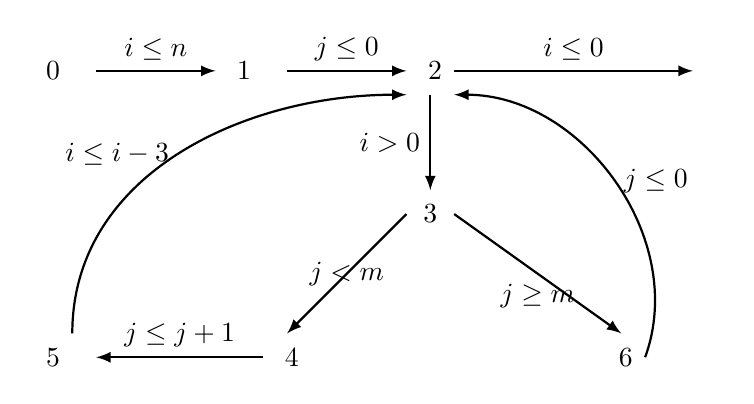
\begin{tikzpicture}[scale=\textwidth/20cm,samples=200]
  \draw[] (-8, 10) circle (0pt) node{{ $0$}};
  \draw[] (-4, 10) circle (0pt) node{{ $1$}};
  \draw[] (0, 10) circle (0pt) node{{ $2$}};
  \draw[] (0, 7) circle (0pt) node{{$3$}};
  \draw[] (-3, 4) circle (0pt) node{{ $4$}};
  \draw[] (-8, 4) circle (0pt) node{{ $5$}};
  \draw[] (4, 4) circle (0pt) node{{ $6$}};
  % Counter Variables
  \draw[] (6, 10) circle (0pt) node {\textbf{$\lex$}};
  % \draw[] (6, 4) circle (0pt) node {{ $ex$}};
  %
  % Control Flow Edges:
  \draw[ thick, -latex] (-7, 10)  -- node [above] {$i \leq n$}(-4.5, 10);
  \draw[ thick, -latex] (-3, 10)  -- node [above] {$j \leq 0$}(-0.5, 10);
  \draw[ thick, -latex] (0, 9.5)  -- node [left] {$i > 0$} (0, 7.5) ;
  \draw[ thick, -latex] (0.5, 7)  -- node [below] {$ j \geq m $}  (4, 4.5);
  \draw[ thick, -latex] (-7.5, 4.5)  to  [out=90,in=180]  node [left] {$i \leq i - 3$ }(-0.5, 9.5);
  \draw[ thick, -latex] (4.5, 4)  to  [out=70,in=0]   node [right] {$j \leq 0 $}(0.5, 9.5);
  \draw[ thick, -latex]  (-0.5, 7) -- node  {$j < m$}  (-3, 4.5) ;
  \draw[ thick, -latex]  (-3.5, 4) -- node [above] {$j \leq j + 1$}  (-7, 4) ;
  \draw[ thick, -latex] (0.5, 10)  -- node [above] {$i \leq 0$}  (5.5, 10);
  % \draw[ thick, -latex] (6, 6.5)  -- node [right] {$\top$} (6, 4.5) ;
  \end{tikzpicture}
  \caption{}
    \end{centering}
    \end{subfigure}
  \caption{
  (a) The Two Paths While Loop Example with Two Coutners
    (b) The Abstract Execution Control Flow Graph}
      \label{fig:twoCountersWhile}
  \end{figure}
  }
\end{example}

\begin{enumerate}
  \item  \textbf{The Abstract Execution Control Flow Graph} is generated in Figure~\ref{fig:twoCountersWhile}(b).

  \item \textbf{Program Rephrase and Refinement}. 
  \\
  The loop free transition paths are computed as follows,
  \[
    \begin{array}{ll}
\tpath_0 = (0 \to 1), (1 \to 2)
&
\tpath_2 = (2 \to 3), (3 \to 6), (6 \to 2)
\\
\tpath_1 = (2 \to 3), (3 \to 4), (4 \to 5), (5 \to 2)
&
\tpath_3 = (2 \to \lex)
\end{array}
\]
\textbf{Rephrased Program}:
\[
\tpath_0 ; LOOP1: \rprepeat(\rpchoose\{\tpath_1, \tpath_2 \}); \tpath_3
\]
\textbf{Refined Program}:
\[
  \tpath_0 ; LOOP1: \rpchoose\{\rprepeat_2(\rprepeat_1(\tpath_1); \tpath_2) , \rprepeat_1(\tpath_1) \}; \tpath_3
  \]
  \item \textbf{Outside-In Algorithm} : Compute Local Bound for Every program and sub programs.
  \[
    \begin{array}{l}
        LB(\tpath_0) = 1
        \\
        LB(\rprepeat_1(\tpath_1)) = m 
        \\
        LB(\rprepeat_2(\rprepeat_1(\tpath_1); \tpath_2)) = \lfloor\frac{n}{m}\rfloor
        \\
        LB(LOOP1: \rpchoose(\rprepeat_2(\cdots), \rprepeat_1(\tpath_1))) 
        = \max\{m, (m  + 1)\times \lfloor\frac{n}{m}\rfloor\}
\end{array}
\]
\item \textbf{Inside-Out Algorithm}
\begin{itemize}
  \item \textbf{Repeat Chain Set}
  \\
  $rp\mathcal{C}(LOOP1, \tpath_1) = \{\rprepeat_1(\tpath_1), \rprepeat_2(\rprepeat_1(\tpath_1); \tpath_2) \to \rprepeat_1(\tpath_1)\}$ \\
  $rp\mathcal{C}(LOOP1, \tpath_2) = \{\rprepeat_2(\cdots; \tpath_2) \to \rprepeat_1(\tpath_1)\}$ \\
  $rp\mathcal{C}(\_, \_) = \emptyset$ 
  % \\
  \item \textbf{{Local Repeat Chain Bound} }for Every Transition Path $\tpath$ on its Repeat Chain
  \\
  $rpLB(LOOP1, \tpath_1) = \max\{m, m \times \lfloor\frac{n}{m}\rfloor\}$ \\
  $rpLB(LOOP1, \tpath_2) = \lfloor\frac{n}{m}\rfloor$ 
  %
  \item \textbf{Loop Chain} Set
  \\
  $lp\mathcal{C}(\tpath_0) = \{\tpath_0\}$ \qquad
  $lp\mathcal{C}(\tpath_1) = \{LOOP1\to \tpath_1\}$ \\
  $lp\mathcal{C}(\tpath_3) = \{\tpath_3\}$ \qquad
  $lp\mathcal{C}(\tpath_2) = \{LOOP1\to \tpath_2\}$ 
  \item \textbf{Nested Loop Bound }for Every Transition Path $\tpath$ on its Loop Chain
  \\
  $rpLB(LOOP1, \tpath_1) = \max\{m, m \times \lfloor\frac{n}{m}\rfloor\}$ \quad
  $rpLB(LOOP1, \tpath_2) = \lfloor\frac{n}{m}\rfloor$  \\
  $rpLB(\bot, \tpath_0) = 1$ \quad
  $rpLB(\bot, \tpath_3) = 1$ 
  \item \textbf{Path Sensitive Reachability Bound For Every Transition Path $\tpath$ }
  \\
  $psRB(\tpath_1) = n$ \quad
  $psRB(\tpath_2) = \lfloor\frac{n}{m}\rfloor$ \quad
  $psRB(\tpath_0) = 1$ \quad
  $psRB(\tpath_3) = 1$ 
\end{itemize}
\item Step 7: Path Sensitive Reachability Bound Computation for Every Location
\\
$psRB(\{0, 1\}) = 1$ \qquad
$psRB(\{\lex\}) = 1$ \qquad
$psRB(\{6 \}) = \lfloor\frac{n}{m}\rfloor$ \\
$psRB(\{4, 5 \}) = \max\{m, m \times \lfloor\frac{n}{m}\rfloor\}$ \quad
$psRB(\{3, 2 \}) = \max\{m, m \times \lfloor\frac{n}{m}\rfloor\} + \lfloor\frac{n}{m}\rfloor + 1 $ \\
\end{enumerate}
\subsection{Three Nested While Loop with Related Iterator Example}
\begin{example}[Nested Loop with Related Iterators]
  \label{ex:threeNestedWhile}
  %
  %
  { \small
\begin{figure}
\centering
\begin{subfigure}{.4\textwidth}
  \begin{centering}
  {\footnotesize
  $
  \begin{array}{l}
      \kw{relatedNestedWhile}(n, m, N) \triangleq \\
      \clabel{ \assign{i}{0} }^{0} ; \\
          \ewhile ~ \clabel{i < n}^{1} ~ \edo ~ \\
          \qquad \Big(
           \clabel{\assign{j}{m}}^{2} ;\\
           \qquad \ewhile ~ \clabel{j > 0}^{3} ~ \edo ~ \\
           \qquad \qquad \Big(
            \clabel{\assign{j}{j-1}}^{4};
            \clabel{\assign{w}{i}}^{5};\\
            \qquad \qquad \ewhile ~ \clabel{w < N}^{6} ~ \edo ~
            \Big(
              \clabel{\assign{w}{w + 1}}^{7}
                \Big); \\
                \qquad \qquad \clabel{\assign{i}{w}}^{8}
                \Big); \\
                \qquad \clabel{\assign{i}{i+1}}^{9}
            \Big)
      \end{array}
  $
  }
  \caption{}
  \end{centering}
  \end{subfigure}
\begin{subfigure}{.5\textwidth}
  \begin{centering}
%   \todo{abstract-cfg for two round}
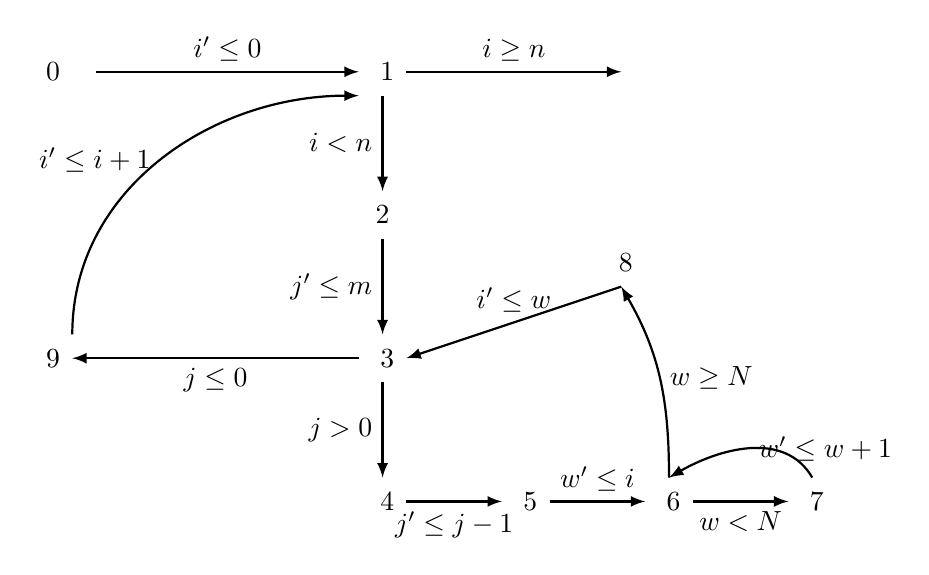
\begin{tikzpicture}[scale=\textwidth/20cm,samples=200]
\draw[] (-7, 10) circle (0pt) node{{ $0$}};
\draw[] (0, 10) circle (0pt) node{{ $1$}};
\draw[] (6, 10) circle (0pt) node {{$\lex$}};
\draw[] (0, 7) circle (0pt) node{{$2$}};
\draw[] (0, 4) circle (0pt) node{{ $3$}};
\draw[] (-7, 4) circle (0pt) node{{ $9$}};
\draw[] (0, 1) circle (0pt) node{{ $4$}};
\draw[] (3, 1) circle (0pt) node{{ $5$}};
\draw[] (6, 1) circle (0pt) node{{ $6$}};
\draw[] (9, 1) circle (0pt) node{{ $7$}};
\draw[] (5, 6) circle (0pt) node{{ $8$}};
% Counter Variables
%
% Control Flow Edges:
\draw[ thick, -latex] (-6, 10)  -- node [above] {$i' \leq 0$}(-0.5, 10);
\draw[ thick, -latex] (0, 9.5)  -- node [left] {$i < n$} (0, 7.5) ;
\draw[ thick, -latex] (0, 6.5)  -- node [left] {$j' \leq m$} (0, 4.5) ;
\draw[ thick, -latex] (0, 3.5)  -- node [left] {$j > 0$} (0, 1.5) ;
\draw[ thick, -latex] (-0.5, 4)  -- node [below] {$j \leq 0$} (-6.5, 4) ;
\draw[ thick, -latex] (-6.5, 4.5)  to  [out=90,in=180]  node [left] {$i' \leq i + 1$ }(-0.5, 9.5);
\draw[ thick, -latex] (0.5, 10)  -- node [above] {$i \geq n$}  (5, 10);
\draw[ thick, -latex] (0.5, 1)  -- node [below] {$j' \leq j - 1$}  (2.5, 1);
\draw[ thick, -latex] (3.5, 1)  -- node [above] {$w' \leq i$}  (5.5, 1);
\draw[ thick, -latex] (6.5, 1)  -- node [below] {$w < N$}  (8.5, 1);
\draw[ thick, -latex] (6, 1.5)  to [out=90,in=-60] node [right] {$w \geq N$}  (5, 5.5);
\draw[ thick, -latex] (9, 1.5)  to  [out=120,in=30] node [right] {$w' \leq w + 1$}  (6, 1.5);
\draw[ thick, -latex] (5, 5.5)  to  node [above] {$i' \leq w$ }(0.5, 4);
\end{tikzpicture}
\caption{}
  \end{centering}
  \end{subfigure}
\caption{
(a) The Example of Nested Loop with Related Iterators
  (b) The Abstract Execution Control Flow Graph}
    \label{fig:threeNestedWhile}
\end{figure}
}
\end{example}

\begin{enumerate}
  \item  \textbf{The Abstract Control Flow Graph}: Figure~\ref{fig:threeNestedWhile}(b).

  \item \textbf{Program Refinement}
  \\
  {Simple Transition Paths:}
  %  are computed as follows,
  \\
$
      \begin{array}{llll}
          \tpath_0 = (0 \to 1)
          &
          \tpath_1 = (1 \to 2 \to 3)
          &           
          \tpath_2 = (3 \to 4 \to 5 \to 6)
          &
          \tpath_3 = (6 \to 7 \to 6)
          \\
          \tpath_6 = (1 \to \lex)
          &
          \tpath_4 = (6 \to 8 \to 3)
          &
          \tpath_5 = (3 \to 9 \to 1)
      \end{array}
$
  \\
  Refined Program:
\\
$
  \rprog = \tpath_0 ; 
1: \rprepeat(\tpath_1; 3: \rprepeat(\tpath_2; 6: \rprepeat(\tpath_3); \tpath_4); \tpath_5); \tpath_6
$
\\
Let $\rprog_1 = \rprepeat(\tpath_1; 3: \rprepeat(\tpath_2; 6: \rprepeat(\tpath_3); \tpath_4); \tpath_5)$
\\
$\rprog_3 = \rprepeat(\tpath_2; 6: \rprepeat(\tpath_3); \tpath_4)$
\\
$\rprog_6 = \rprepeat(\tpath_3)$
  \item {Path Local Reachability-bound}:
\\
$\outinB(1: \rprog_1, \tpath_1) = n - N$ \quad
$\outinB(1: \rprog_1, \tpath_5) = n - N$ \quad
$\outinB(3: \rprog_3, \tpath_2) = m$ \\
$\outinB(3: \rprog_3, \tpath_4) = m$ \quad
$\outinB(6: \rprog_6, \tpath_3) = N$ \quad
%
\\
Loop Bounds:
\\
$BD(\tpath_0) = 1$
\quad
$BD(\tpath_6) = 1$
\quad
$BD( \rprepeat(\tpath_3)) = N $
\quad
$BD(\rprog_3) = m $
\quad
$BD(\rprog_1) = n - N $
%
\item Loop Reachability-bound:
\\
\highlight{
$\lpchB(1: \rprog_1, \tpath_1) = n - N$ \quad
$\lpchB(1: \rprog_1, \tpath_5) = n - N$ \quad
$\lpchB(1: \rprog_1, \tpath_2) = n$ \\ 
$\lpchB(1: \rprog_1, \tpath_4) = n$ \quad
$\lpchB(1: \rprog_1, \tpath_3) = 1$ \quad
$\lpchB(3: \rprog_3, \tpath_4) = m$ \\
$\lpchB(3: \rprog_3, \tpath_2) = m$ \quad
$\lpchB(3: \rprog_3, \tpath_3) = 1$ \quad 
$\lpchB(6: \rprog_6, \tpath_3) = N$
}
%
%
\item Path Global Reachability-bound:
\\
$\inoutB(\rprog, \tpath_1) = n - N$ \quad
$\inoutB(\rprog, \tpath_2) = n \times m$ \quad
$\inoutB(\rprog, \tpath_0) = 1$ 
\quad
$\inoutB(\rprog, \tpath_5) = n - N$ \quad
$\inoutB(\rprog, \tpath_4) = n \times m$ \quad
$\inoutB(\rprog, \tpath_6) = 1$ 
\quad
$\inoutB(\rprog, \tpath_3) = N$
%
\item The Reachability-bound:
\\
$\psRB(0) = \psRB(\lex) = 1$ \quad
$\psRB(1) = n - N + 1$ \quad
$\psRB(2) = \psRB(9) = n - N$ \quad
$\psRB(7) = N$
\\
$\psRB(3) = n - N + n \times m$ \quad
$\psRB(4) = \psRB(5) = \psRB(8) = n \times m$ \quad
$\psRB(6) = N + n \times m$ 
\end{enumerate}
\subsection{Simplified Nested Loop with Related Iterator Example}
\begin{example}[A Simplified Nested Loop with Related Iterator Example]
  \label{ex:relatedNestedWhileSim}
  %
  %
  { \small
\begin{figure}
\centering
\begin{subfigure}{.4\textwidth}
  \begin{centering}
  {\footnotesize
  $
  \begin{array}{l}
      \kw{relatedNestedWhileSim}(n, m, N) \triangleq \\
      \clabel{ \assign{i}{0} }^{0} ; \\
          \ewhile ~ \clabel{i < n}^{1} ~ \edo ~ \\
          \qquad \Big(
            \clabel{\assign{w}{i}}^{2};\\
            \qquad \ewhile ~ \clabel{w < N}^{3} ~ \edo ~
            \Big(
              \clabel{\assign{w}{w + 1}}^{4}
                \Big); \\
                \qquad \clabel{\assign{i}{w}}^{5};
                \clabel{\assign{i}{i+1}}^{6}
            \Big)
      \end{array}
  $
  }
  \caption{}
  \end{centering}
  \end{subfigure}
\begin{subfigure}{.5\textwidth}
  \begin{centering}
%   \todo{abstract-cfg for two round}
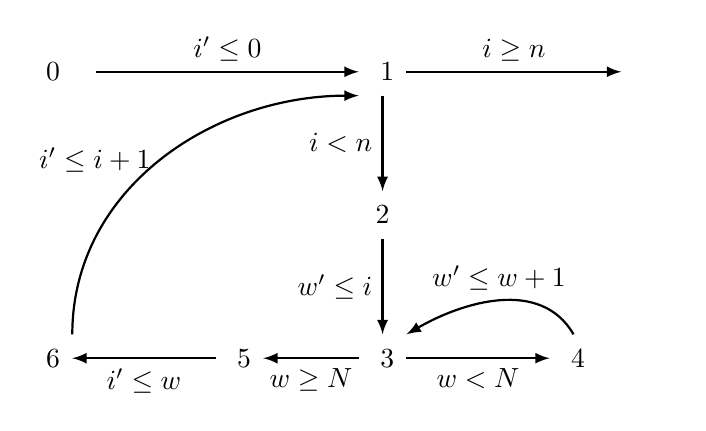
\begin{tikzpicture}[scale=\textwidth/20cm,samples=200]
\draw[] (-7, 10) circle (0pt) node{{ $0$}};
\draw[] (0, 10) circle (0pt) node{{ $1$}};
\draw[] (6, 10) circle (0pt) node {{$\lex$}};
\draw[] (0, 7) circle (0pt) node{{$2$}};
\draw[] (0, 4) circle (0pt) node{{ $3$}};
\draw[] (-7, 4) circle (0pt) node{{ $6$}};
\draw[] (-3, 4) circle (0pt) node{{ $5$}};
\draw[] (4, 4) circle (0pt) node{{ $4$}};
% Counter Variables
%
% Control Flow Edges:
\draw[ thick, -latex] (-6, 10)  -- node [above] {$i' \leq 0$}(-0.5, 10);
\draw[ thick, -latex] (0, 9.5)  -- node [left] {$i < n$} (0, 7.5) ;
\draw[ thick, -latex] (0, 6.5)  -- node [left] {$w' \leq i$} (0, 4.5) ;
\draw[ thick, -latex] (-0.5, 4)  -- node [below] {$w \geq N$} (-2.5, 4) ;
\draw[ thick, -latex] (-3.5, 4)  -- node [below] {$i' \leq w$} (-6.5, 4) ;
\draw[ thick, -latex] (-6.5, 4.5)  to  [out=90,in=180]  node [left] {$i' \leq i + 1$ }(-0.5, 9.5);
\draw[ thick, -latex] (0.5, 10)  -- node [above] {$i \geq n$}  (5, 10);
\draw[ thick, -latex] (4, 4.5)  to  [out=120,in=30] node [above] {$w' \leq w + 1$}  (0.5, 4.5);
\draw[ thick, -latex] (0.5, 4)  -- node [below] {$w < N$}  (3.5, 4);
\end{tikzpicture}
\caption{}
  \end{centering}
  \end{subfigure}
\caption{
(a) The Simplified Example of Nested Loop with Related Iterator
  (b) The Abstract Execution Control Flow Graph}
    \label{fig:relatedNestedWhileSim}
\end{figure}
}
\end{example}

\begin{enumerate}
  \item  \textbf{The Constraint Program (Abstract Control Flow Graph)} is generated in Figure~\ref{fig:threeNestedWhile}(b).

  \item \textbf{Program Refinement}
  \\
  The loop free simple transition paths are computed as follows,
  \[
      % \begin{array}{lllll}
          \tpath_0 = (0 \to 1)
          \quad
          \tpath_1 = (1 \to 2 \to 3)
          \quad           
          \tpath_2 = (3 \to 4 \to 3)
          \quad
          \tpath_3 = (3 \to 5 \to 6 \to 1)
          \quad
          \tpath_4 = (1 \to \lex)
      % \end{array}
      \]
  \textbf{Refined Program}:
  \[
  \rprog = \tpath_0 ; 1: \rprepeat(\tpath_1; 3: \rprepeat(\tpath_2); \tpath_3); \tpath_4
  \]
  \item \textbf{Outside-In Algorithm}: The \emph{OutIn} bound for the $\rprog$ and every nested repeat patterns.
  \\
$\outinB(\tpath_0) = 1$
\quad
$\outinB(3: \rprepeat(\tpath_2)) = N $
\\
$\outinB(1: \rprepeat(\tpath_1; 3: \rprepeat(\tpath_2); \tpath_3)) = n - N $
\item \textbf{Inside-Out Algorithm}
\begin{itemize}
  \item \textbf{Repeat Chain Set}
  \\
  $\rpchset(1, \tpath_1) = \{\rprepeat(\tpath_1; 3: \rprepeat(\tpath_2); \tpath_3)\}$
  \\
  $\rpchset(1, \tpath_3) = \{\rprepeat(\tpath_1; 3: \rprepeat(\tpath_2); \tpath_3)\}$
  \\
  $\rpchset(3, \tpath_2) = \{\rprepeat(\tpath_2)\}$ \quad
  $\rpchset(_, \_) = \emptyset$ 
  % \\
  \item \textbf{Repeat Chain Bound} for every simple transition path $\tpath$ through its \emph{Repeat Chain}s
  \\
  $\rpchB(1, \tpath_1) = n - N$ \quad
  $\rpchB(1, \tpath_3) = n - N$ \quad
  $\rpchB(3, \tpath_2) = N$ \quad
  $\rpchB(_, \_) = \bot $ 
  %
  \item \textbf{Loop Chain}
  \\
  $\lpch(\tpath_1) = 1\to \tpath_1$ \quad
  \highlight{$\lpch(\tpath_2) = 1 \to 3 \to \tpath_2$} \quad
  $\lpch(\tpath_3) = 1 \to \tpath_3$ \\
  $\lpch(\tpath_0) = \tpath_0$ \quad
  $\lpch(\tpath_4) = \tpath_4$
  \item \textbf{{Relative Loop Bound}} for every simple transition path $\tpath$ through its \emph{Loop Chain}
  \\
  $\rpchB(1, \tpath_1) = n - N$ \quad
  $\rpchB(1, \tpath_3) = n - N$ \quad
  \highlight{$\rpchB(1, \tpath_2) = 1$} \quad
  $\rpchB(3, \tpath_2) = N$ \quad
  $\rpchB(_, \_) = 1 $ 
  \item \textbf{Path-Sensitive Reachability-Bound} for every simple transition path $\tpath$
  \\
  $\inoutB(\tpath_1) = n - N$ \quad
  $\inoutB(\tpath_2) = N$ \quad
  $\inoutB(\tpath_0) = 1$ 
  \\
  \highlight{ $\inoutB(\tpath_3) = n - N$} \quad
  $\inoutB(\tpath_4) = 1$ 
  \end{itemize}
\item \textbf{Path Sensitive Reachability-Bound} on every program control location
\\
$\psRB(\{0, \lex\}) = 1$ \quad
$\psRB(\{1\}) = n - N + 1$ \quad
$\psRB(\{2, 5, 6\}) = n - N$ \\
\highlight{$\psRB(\{3\}) = N + 1 + n - N = n + 1$} \quad
$\psRB(\{4\}) = N$
\end{enumerate}
\subsection{Nested Loop with Iterator Reset Chain Example}
\begin{example}[Nested Loop with Variable Reset Chain]
  \label{ex:nestedWhileResetChain}
  %
  %
  { \small
\begin{figure}
\centering
\begin{subfigure}{.4\textwidth}
  \begin{centering}
  {\small
  $
  \begin{array}{l}
      \kw{nestedWhileResetChain}(n) \triangleq \\
      \clabel{ \assign{i}{n} }^{0} ; \\
      \clabel{ \assign{r}{n} }^{1} ; \\
          \ewhile ~ \clabel{i > 0}^{2} ~ \edo ~ \\
          \qquad \Big( \clabel{\assign{r}{r + 1}}^{3};\\
            \qquad  \clabel{\assign{k}{r}}^{4};\\
            \qquad \ewhile ~ \clabel{k > 0}^{5} ~ \edo ~
            \Big( \clabel{\assign{k}{k - 1}}^{6}   \Big); \\
                \qquad \clabel{\assign{r}{k}}^{7};
                \clabel{\assign{i}{i-1}}^{8}
            \Big)
      \end{array}
  $
  }
  \caption{}
  \end{centering}
  \end{subfigure}
\begin{subfigure}{.5\textwidth}
  \begin{centering}
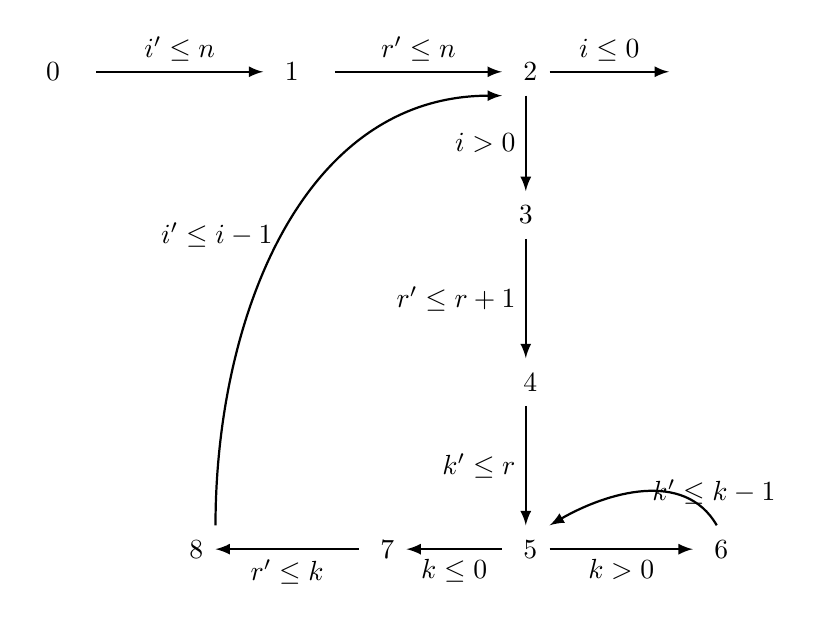
\begin{tikzpicture}[scale=\textwidth/20cm,samples=200]
\draw[] (-10, 10) circle (0pt) node{{ $0$}};
\draw[] (-5, 10) circle (0pt) node{{ $1$}};
\draw[] (0, 10) circle (0pt) node{{ $2$}};
\draw[] (4, 10) circle (0pt) node {{$\lex$}};
%
\draw[] (0, 7) circle (0pt) node{{$3$}};
\draw[] (0, 3.5) circle (0pt) node{{ $4$}};
\draw[] (0, 0) circle (0pt) node{{ $5$}};
\draw[] (4, 0) circle (0pt) node{{ $6$}};
%
\draw[] (-3, 0) circle (0pt) node{{ $7$}};
\draw[] (-7, 0) circle (0pt) node{{ $8$}};
% Counter Variables
%
% Control Flow Edges:
\draw[ thick, -latex] (-9, 10)  -- node [above] {$i' \leq n$}(-5.5, 10);
\draw[ thick, -latex] (-4, 10)  -- node [above] {$r' \leq n$}(-0.5, 10);
\draw[ thick, -latex] (0.5, 10)  -- node [above] {$i \leq 0 $}  (3, 10);
\draw[ thick, -latex] (0, 9.5)  -- node [left] {$i > 0$} (0, 7.5) ;
\draw[ thick, -latex] (0, 6.5)  -- node [left] {$r' \leq r + 1$} (0, 4) ;
\draw[ thick, -latex] (0, 3)  -- node [left] {$k' \leq r$} (0, 0.5) ;
% While Guard True, Loop Body
\draw[ thick, -latex] (0.5, 0)  -- node [below] {$k > 0$}  (3.5, 0);
\draw[ thick, -latex] (4, 0.5)  to  [out=120,in=30] node [right] {$k' \leq k - 1$}  (0.5, 0.5);
% While Guard IS FALSE, RETURN BACK TO THE PREVIOUS CONTROL POINT
\draw[ thick, -latex] (-0.5, 0)  -- node [below] {$k \leq 0$} (-2.5, 0) ;
\draw[ thick, -latex] (-3.5, 0)  -- node [below] {$r' \leq k$} (-6.5, 0) ;
\draw[ thick, -latex] (-6.5, 0.5)  to  [out=90,in=180]  node [left] {$i' \leq i - 1$ }(-0.5, 9.5);
\end{tikzpicture}
\caption{}
  \end{centering}
  \end{subfigure}
\caption{
(a) The Simplified Example of Nested Loop with Related Iterator
  (b) The Abstract Execution Control Flow Graph}
    \label{fig:nestedWhileResetChain}
\end{figure}
}
\end{example}

\begin{enumerate}
  \item  \textbf{Abstract Control Flow Graph} is generated in Figure~\ref{fig:nestedWhileResetChain}(b).

  \item \textbf{Program Refinement}
  \\
  The loop free simple transition paths:
  \[
      % \begin{array}{lllll}
          \tpath_0 = (0 \to 1 \to 2)
          \quad
          \tpath_1 = (2 \to 3 \to 4 \to 5)
          \quad           
          \tpath_2 = (5 \to 6 \to 5)
          \quad
          \tpath_3 = (5 \to 7 \to 8 \to 2)
          \quad
          \tpath_4 = (2 \to \lex)
      % \end{array}
      \]
  \textbf{Refined Program}:
  \[
  \rprog = \tpath_0 ; 2: \rprepeat(\tpath_1; 5: \rprepeat(\tpath_2); \tpath_3); \tpath_4
  \]
Let $\rprog_2 = \rprepeat(\tpath_1; 5: \rprepeat(\tpath_2); \tpath_3)$
\item {Path Local Reachability Bound}:
\\
$\outinB(\rprog, \tpath_0) = 1$ \quad
$\outinB(\rprog, \tpath_4) = 1$ \\
$\outinB(2: \rprog_2, \tpath_1) = n$ \quad
$\outinB(2: \rprog_2, \tpath_3) = n$ \\
$\outinB(5: \rprepeat(\tpath_2), \tpath_2) = n + 1$
%
\\
Loop Bounds:
\\
$BD(\tpath_0) = 1$
\quad
$BD(\tpath_4) = 1$
\quad
$BD(\rprepeat(\tpath_2)) = n + 1 $
\\
$BD(\rprepeat(\tpath_1; 5: \rprepeat(\tpath_2); \tpath_3)) = n $
%
\item Loop Reachability Bound:
\\
\highlight{
$\lpchB(2: \rprog_2, \tpath_1) = n$ \quad
$\lpchB(2: \rprog_2, \tpath_3) = n$ \quad 
$\lpchB(2: \rprog_2, \tpath_2) = \frac{(n + 1) - 0}{n}$ 
\\
$\lpchB(5: \rprepeat(\tpath_2), \tpath_2) = n + 1$ \\
$\lpchB(2: \rprog_2, \tpath_4) = 0$ \quad
$\lpchB(2: \rprog_2, \tpath_0) = 0$ \quad
$\lpchB(2: \rprog_2, \tpath_0) = 0$ \quad
}
%
%
\item Path Global Reachability Bound:
\\
$\inoutB(\rprog, \tpath_0) = 1$ \quad
$\inoutB(\rprog, \tpath_1) = n$ \quad
$\inoutB(\rprog, \tpath_2) = \frac{(n + 1)^2}{n}$ \\
$\inoutB(\rprog, \tpath_3) = n$ \quad
$\inoutB(\rprog, \tpath_4) = 1$
%
\item The Reachability Bound:
\\
$\psRB(0) = \psRB(1) = \psRB(\lex) = 1$ \quad
$\psRB(2) = n + 1$ \\
$\psRB(3) = \psRB(4) =\psRB(7) = \psRB(8) = n$ \quad \\
$\psRB(6) = \frac{(n + 1)^2}{n} $ \quad
\highlight{$\psRB(\{5\}) = n + \frac{(n + 1)^2}{n}$}
\end{enumerate}
\subsection{Two Paths Loop with Nested Loop in One Path}
\begin{example}
  [Example with Two Paths Iterating Alternatively and Nested Loop in One Path]
  \label{ex:nestedWhileOdd}
  { \small
  \begin{figure}
  \centering
  \begin{subfigure}{.4\textwidth}
    \begin{centering}
    {\small
    $
    \begin{array}{l}
      \kw{nestedWhileOdd}(k) \triangleq \\
      \clabel{ \assign{i}{k} }^{0} ; \\
          \ewhile ~ \clabel{i > 0}^{1} ~ \edo ~ \\
          \qquad \Big(
            \eif(\clabel{i \% 2 = 0 }^{2},\\
            \qquad \clabel{\assign{i}{i - 1}}^{3};
            \clabel{\assign{j}{k}}^{4}; \\
            \qquad \ewhile ~ \clabel{j > 0}^{5} ~ \edo ~
            \Big( \clabel{\assign{j}{j - 1}}^{6} \Big),\\
            \qquad \clabel{\assign{i}{i - 3}}^{7});
            \Big)
      \end{array}
    $
    }
    \caption{}
    \end{centering}
    \end{subfigure}
  \begin{subfigure}{.5\textwidth}
    \begin{centering}
  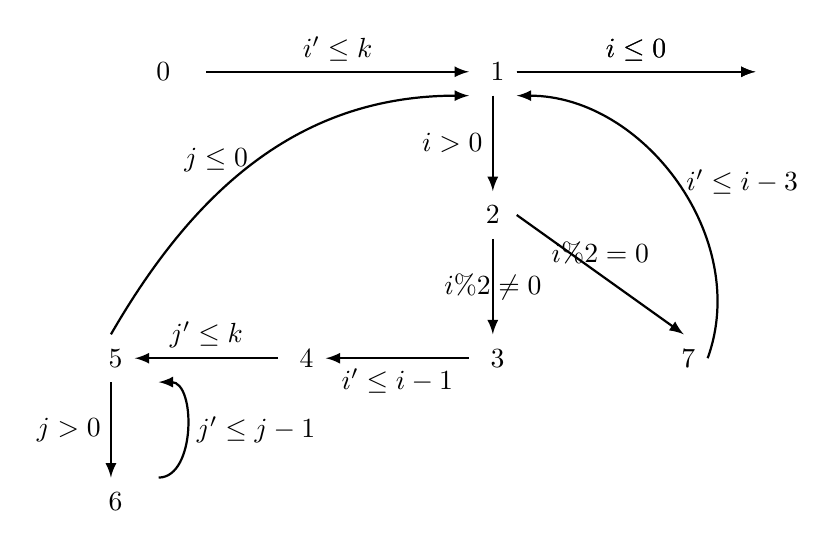
\begin{tikzpicture}[scale=\textwidth/20cm,samples=200]
  \draw[] (-7, 10) circle (0pt) node{{ $0$}};
  \draw[] (0, 10) circle (0pt) node{{ $1$}};
  \draw[] (0, 7) circle (0pt) node{\textbf{$2$}};
  \draw[] (0, 4) circle (0pt) node{{ $3$}};
  \draw[] (-4, 4) circle (0pt) node{{ $4$}};
  \draw[] (-8, 4) circle (0pt) node{{ $5$}};
  \draw[] (-8, 1) circle (0pt) node{{ $6$}};
  \draw[] (4, 4) circle (0pt) node{{ $7$}};
  % Counter Variables
  \draw[] (6, 10) circle (0pt) node {\textbf{$\lex$}};
  % \draw[] (6, 4) circle (0pt) node {{ $ex$}};
  %
  % Control Flow Edges:
  \draw[ thick, -latex] (-6, 10)  -- node [above] {$i' \leq k$}(-0.5, 10);
  \draw[ thick, -latex] (0, 9.5)  -- node [left] {$i > 0$} (0, 7.5) ;
  \draw[ thick, -latex] (0.5, 7)  -- node [above] {$ i \% 2 = 0 $}  (4, 4.5);
  \draw[ thick, -latex] (-8, 4.5)  to  [out=60,in=180]  node [left] {$j \leq 0$ }(-0.5, 9.5);
  \draw[ thick, -latex] (4.5, 4)  to  [out=70,in=0]   node [right] { $i' \leq i - 3$ }(0.5, 9.5);
  \draw[ thick, -latex]  (0, 6.5) -- node  {$i \% 2 \neq 0$}  (0, 4.5) ;
  \draw[ thick, -latex]  (-0.5, 4) -- node [below] {$i' \leq i - 1$ }  (-3.5, 4) ;
  \draw[ thick, -latex]  (-4.5, 4) -- node [above] {$j' \leq k$ }  (-7.5, 4);
  \draw[ thick, -latex] (0.5, 10)  -- node [above] {$i \leq 0$}  (5.5, 10);
  \draw[ thick, -latex] (-8, 3.5)  -- node [left] {$j > 0$}  (-8, 1.5);
  \draw[ thick, -latex] (-7, 1.5)  to  [out=0,in=0] node [right] {$j' \leq j - 1$}  (-7, 3.5);
  \draw[ thick, -latex] (0.5, 10)  -- node [above] {$i \leq 0$}  (5.5, 10);
  % \draw[ thick, -latex] (6, 6.5)  -- node [right] {$\top$} (6, 4.5) ;
  \end{tikzpicture}
  \caption{}
    \end{centering}
    \end{subfigure}
  \caption{
  (a) The program of the two paths loop with a nested Loop in one path
    (b) The Abstract Execution Control Flow Graph}
      \label{fig:nestedWhileOdd}
  \end{figure}
  }
  %
  \end{example}    
  \begin{enumerate}
    \item  \textbf{The Abstract Execution Control Flow Graph} is generated in Figure~\ref{fig:nestedWhileOdd}(b).
    \item \textbf{Program Refinement}
    \\
    The loop free simple transition paths are computed as follows,
      \\ 
    $\tpath_0 = (0 \to 1)$
      \quad
      $\tpath_1 = (1 \to 2 \to 3 \to 4 \to 5)$
      \quad
      $\tpath_2 = (5 \to 6 \to 5)$
      \quad
      $\tpath_3 = (1 \to 7 \to 2 \to 1)$
      \quad
      $\tpath_4 = (1 \to \lex)$
      \quad
      $\tpath_5 = (5 \to 1)$

  \textbf{Refined Program}:
  \[
    \tpath_0 ; \rpchoose{1: \rprepeat(\tpath_1; 5:\rprepeat(\tpath_2); \tpath_3) , 
    1: \rprepeat(\tpath_3; \tpath_1; 5:\rprepeat(\tpath_2); \tpath_5 )}; \tpath_4
    \]
    Let $\rprog_1^1 = \rprepeat(\tpath_1; 5:\rprepeat(\tpath_2); \tpath_3)$
    \\
    $\rprog_1^2 = \rprepeat(\tpath_3; \tpath_1; 5:\rprepeat(\tpath_2) ; \tpath_5 )$
    \item {Path Local Reachability-bound}:
    \\
    $\outinB(\rprog, \tpath_0) = 1$ \\
    $\outinB(\rprog, \tpath_4) = 1$ \\
    $\outinB(1: \rprog_1^1, \tpath_1) = \frac{n}{4}$ \\
    $\outinB(1: \rprog_1^1, \tpath_3) = \frac{n}{4}$ \\
    $\outinB(1: \rprog_1^1, \tpath_5) = \frac{n}{4}$ \\
    $\outinB(1: \rprog_1^2, \tpath_1) = \frac{n}{4}$ \\
    $\outinB(1: \rprog_1^2, \tpath_3) = \frac{n}{4}$ \\
    $\outinB(1: \rprog_1^2, \tpath_5) = \frac{n}{4}$ \\
    $\outinB(5: \rprepeat(\tpath_2), \tpath_2) = n$ 
    \\
    Loop Bounds:
    \\
    $BD(\tpath_0) = 1$
    \quad
    $BD(\tpath_4) = 1$
    \quad
    $BD(\rprepeat(\tpath_2)) = n $
    \quad
    $BD(\rprog_1^1) = \frac{n}{4} $
    \quad
    $BD(\rprog_1^2) = \frac{n}{4} $

    %
    \item Loop Reachability-bound:
    \\
    \highlight{
    $\lpchB(1: \rprog_1^1, \tpath_1) = \frac{n}{4}$ \quad
    $\lpchB(1: \rprog_1^1, \tpath_3) = \frac{n}{4}$ \quad 
    $\lpchB(1: \rprog_1^1, \tpath_5) = \frac{n}{4}$ \quad 
    \highlight{$\lpchB(1: \rprog_1^1, \tpath_2) = \frac{n}{4}$} \\ 
    $\lpchB(1: \rprog_1^2, \tpath_1) = \frac{n}{4}$ \quad
    $\lpchB(1: \rprog_1^2, \tpath_3) = \frac{n}{4}$ \quad 
    $\lpchB(1: \rprog_1^2, \tpath_5) = \frac{n}{4}$ \quad 
    \highlight{$\lpchB(1: \rprog_1^2, \tpath_2) = \frac{n}{4}$} \\
    $\lpchB(5: \rprepeat(\tpath_2), \tpath_2) = n$ \quad
    }
    %
    %
    \item Path Global Reachability-bound:
    \\
    $\inoutB(\rprog, \tpath_0) = 1$ \quad
    $\inoutB(\rprog, \tpath_1) = \frac{n}{4}$ \quad
    $\inoutB(\rprog, \tpath_2) = \frac{n}{4} \times n$ \\
    $\inoutB(\rprog, \tpath_3) = \frac{n}{4}$ \quad
    $\inoutB(\rprog, \tpath_5) = \frac{n}{4}$ \quad
    $\inoutB(\rprog, \tpath_4) = 1$
    %
    \item The Reachability-bound:
    \\
    $\psRB(0) = \psRB(\lex) = 1$ \quad
    $\psRB(1) = \frac{n}{2} + 1$ \quad
    $\psRB(2) = \frac{n}{2} $ \\
    $\psRB(3) = \psRB(4) = \psRB(7) = \frac{n}{4} $ \\
    \highlight{$\psRB(6) = \frac{n}{4} \times n$} \\
    $\psRB(5) =  \frac{n}{4} \times (n + 1)$
  \end{enumerate}

\subsection{Two Paths Loop with Alternative Iterations}
\begin{example}
    [While Odds Algorithm]
    \label{ex:whileOdd}
    \[
      %
      \begin{array}{l}
          \kw{whileOdd}(k) \triangleq \\
          \clabel{ \assign{i}{k} }^{0} ; \\
              \ewhile ~ \clabel{i > 0}^{1} ~ \edo ~ \\
              \qquad \Big(
                \eif(\clabel{i \% 2 == 0 }^{2}, \\
                \qquad \qquad \clabel{\assign{i}{i - 1}}^{3},\\
                \qquad \qquad \clabel{\assign{i}{i - 3}}^{4});
                \Big)
          \end{array}
      \]
    % \end{example}
    { \small
    \begin{figure}
    \centering
    %
    \begin{subfigure}{.4\textwidth}
        \begin{centering}
        \begin{tikzpicture}[scale=\textwidth/15cm,samples=200]
    % Variables Initialization
    \draw[] (5, 1) circle (0pt) node{{ $x^1: {}^1_{1}$}};
    % Variables Inside the Loop
     \draw[] (0, 7) circle (0pt) node{\highlight{ $y^5: {}^{\frac{k}{2}}_{1}$}};
     \draw[] (0, 4) circle (0pt) node{\highlight{ \boldsymbol{$p^6: {}^{\frac{k}{2}}_{1}$}}};
     \draw[] (0, 1) circle (0pt) node{{ $\mathbf{x^7: {}^{k}_{1}}$}};
     % Counter Variables
     \draw[] (5, 7) circle (0pt) node {{$j^0: {}^{1}_{0}$}};
     \draw[] (5, 4) circle (0pt) node {{ $j^3: {}^{k}_{0}$}};
     %
    % Value Dependency Edges:
             % Value Dependency Edges:
             \draw[ thick, -latex,]  (0, 3.5) -- 
             node [] {\highlight{$k $}}(0, 1.5) ;
             \draw[ thick, -Straight Barb] (6.5, 4.5) arc (150:-150:1);
             \draw[](7, 4) node [] {\highlight{$k  $}};
             \draw[ thick, -latex] (5, 4.5)  -- 
             node [right] {\highlight{$k$}}(5, 6.5) ;
             % Value Dependency Edges on Initial Values:
             \draw[ thick, -latex,] (1.5, 1)  -- 
             node [above] {\highlight{$k$}}(4, 1) ;
             %
            \draw[ ultra thick, -latex, densely dotted,] (-0.6, 1.5)  to  [out=-220,in=220]  
            node [left] {\highlight{$k $}}(-0.5, 6.5);
            \draw[ ultra thick, -latex, densely dotted,]  (0.5, 6.5) to  [out=-30,in=30] 
            node [above] {\highlight{$k $}}(0.6, 1.6) ;
             % Control Dependency
            \draw[ thick,-latex] (1.5, 7)  -- 
            node [above] {\highlight{$k$}}(4, 6) ;
            \draw[ thick,-latex] (1.5, 4)  -- 
            node [above] {\highlight{$k$}}(4, 6) ;
             \draw[ thick,-latex] (1.5, 1)  -- 
             node [below] {\highlight{$k $}}(4, 6) ;
    
    \end{tikzpicture}
    \caption{}
    \end{centering}
    \end{subfigure}
    %
            \begin{subfigure}{.5\textwidth}
                \begin{centering}
                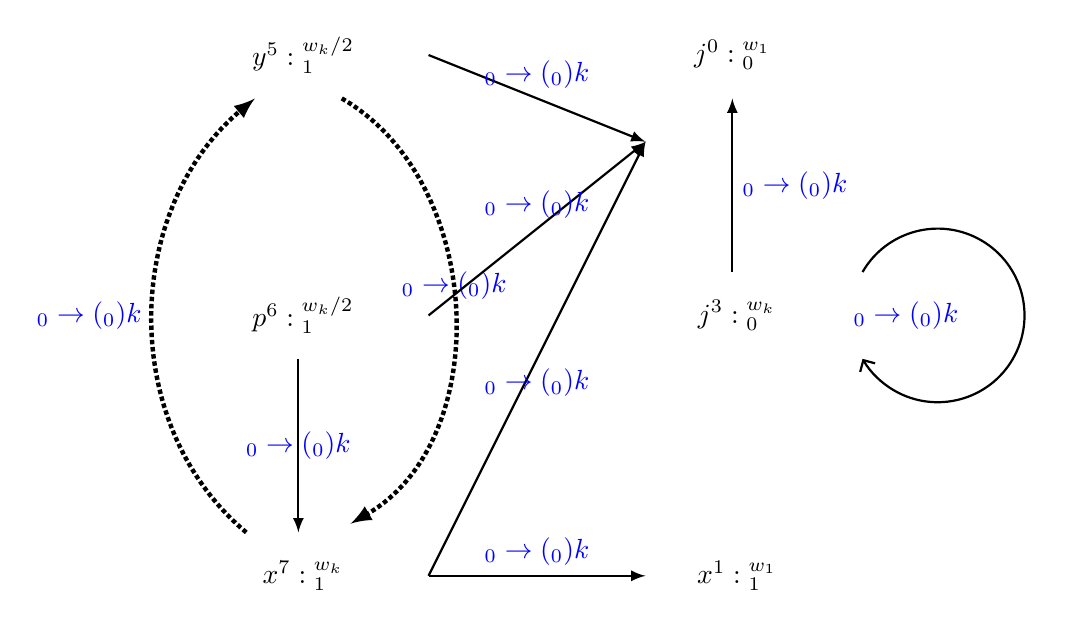
\begin{tikzpicture}[scale=\textwidth/11cm,samples=200]
            % Variables Initialization
             \draw[] (5, 1) circle (0pt) node{{ $x^1: {}^{w_1}_{1}$}};
            % Variables Inside the Loop
             \draw[] (0, 7) circle (0pt) node{{ $y^5: {}^{w_k/2}_{1}$}};
             \draw[] (0, 4) circle (0pt) node{{ $p^6: {}^{w_k/2}_{1}$}};
             \draw[] (0, 1) circle (0pt) node{{ $x^7: {}^{w_k}_{1}$}};
             % Counter Variables
             \draw[] (5, 7) circle (0pt) node {{$j^0: {}^{w_1}_{0}$}};
             \draw[] (5, 4) circle (0pt) node {{ $j^3: {}^{w_k}_{0}$}};
             %
             % Value Dependency Edges:
             \draw[ thick, -latex,]  (0, 3.5) -- 
             node [] {\highlight{$\trace_0 \to \env(\trace_0) k $}}(0, 1.5) ;
             \draw[ thick, -Straight Barb] (6.5, 4.5) arc (150:-150:1);
             \draw[](7, 4) node [] {\highlight{$\trace_0 \to \env(\trace_0) k  $}};
             \draw[ thick, -latex] (5, 4.5)  -- 
             node [right] {\highlight{$\trace_0 \to \env(\trace_0) k $}}(5, 6.5) ;
             % Value Dependency Edges on Initial Values:
             \draw[ thick, -latex,] (1.5, 1)  -- 
             node [above] {\highlight{$\trace_0 \to \env(\trace_0) k $}}(4, 1) ;
             %
            \draw[ ultra thick, -latex, densely dotted,] (-0.6, 1.5)  to  [out=-220,in=220]  
            node [left] {\highlight{$\trace_0 \to \env(\trace_0) k $}}(-0.5, 6.5);
            \draw[ ultra thick, -latex, densely dotted,]  (0.5, 6.5) to  [out=-30,in=30] 
            node [above] {\highlight{$\trace_0 \to \env(\trace_0) k $}}(0.6, 1.6) ;
             % Control Dependency
            \draw[ thick,-latex] (1.5, 7)  -- 
            node [above] {\highlight{$\trace_0 \to \env(\trace_0) k $}}(4, 6) ;
            \draw[ thick,-latex] (1.5, 4)  -- 
            node [above] {\highlight{$\trace_0 \to \env(\trace_0) k $}}(4, 6) ;
             \draw[ thick,-latex] (1.5, 1)  -- 
             node [below] {\highlight{$\trace_0 \to \env(\trace_0) k $}}(4, 6) ;
             \end{tikzpicture}
             \caption{}
                \end{centering}
                \end{subfigure}
    \caption{
    (a) The multiple rounds odd example 
    (b) The program-based dependency graph from $\THESYSTEM$
    (c) The execution-based dependency graph.}
        \label{fig:overappr_example}
    \end{figure}
    }
    %
    \end{example}    
    \begin{enumerate}
      \item Step 1: Abstract Transition Graph:
    
    \item Step 2: Path Insensitive Transition Bound Computation
    
    \item Step 3: Program Rephrase through Path Collection on Abstract CFG
    \\
    $\tpath_0 = (0, 1)$
    \\
    $\tpath_1 = (1 \to 2), (2 \to 3), (3 \to 1)$
    \\
    $\tpath_2 = (1 \to 2), (2 \to 4), (4 \to 1)$
    \\
    $\tpath_3 = (1 \to \lex)$
    \\
    Rephrased Program
    \[
    \tpath_0 ; LOOP1: \rprepeat(\rpchoose\{\tpath_1, \tpath_2 \}); \tpath_3
    \]
    \item Step 4: While Loop Refinement:
    \[
      \tpath_0 ; LOOP1: \rpchoose\{\rprepeat_3(\rprepeat_1(\tpath_1); \tpath_2) , \rprepeat_4(\rprepeat_2(\tpath_2); \tpath_1) \}; \tpath_3
      \]
    \item Step 5: Outside-In Algorithm
    \\
    $LB(\tpath_0) = 1$
    \\
    $LB(\tpath_3) = 1$
    \\
    $LB(\rprepeat_1(\tpath_1)) = 1 $
    \\
    $LB(\rprepeat_3(\rprepeat_1(\tpath_1); \tpath_2)) = \frac{n}{4} $
    \\
    $LB(\rprepeat_2(\tpath_2)) = 1 $
    \\
    $LB(\rprepeat_4(\rprepeat_2(\tpath_2); \tpath_1)) = \frac{n}{4} $
    % \\
    % $LB(LOOP1: \rpchoose(\rprepeat_2(\cdots), \rprepeat_1(\tpath_1))) 
    % = \max\{m, \frac{n}{m}\} $
    % \\
    \item Step 6: Inside-Out Algorithm
    \begin{itemize}
      \item \textbf{Repeat Chain Set}
      \\
      $rp\mathcal{C}(LOOP1, \tpath_1) = \{\rprepeat_4(\cdots, \tpath_1), \rprepeat_3(\rprepeat_1(\tpath_1); \tpath_2) \to \rprepeat_1(\tpath_1)\}$ \\
      $rp\mathcal{C}(LOOP1, \tpath_2) = \{\rprepeat_3(\cdots, \tpath_2), \rprepeat_4(\rprepeat_2(\tpath_2); \tpath_1) \to \rprepeat_2(\tpath_2)\}$ \\
      $rp\mathcal{C}(\_, \_) = \emptyset$ 
      % \\
      \item \textbf{{Local Repeat Chain Bound} for Every Transition Path $\tpath$ on its Repeat Chain}
      $rpLB(LOOP1, \tpath_1) = \frac{n}{4}$ \\
      $rpLB(LOOP1, \tpath_2) = \frac{n}{4}$ 
      %
      \item \textbf{Loop Chain}
      \\
      $lp\mathcal{C}(\tpath_1) = \{LOOP1\to \tpath_1\}$ \\
      $lp\mathcal{C}(\tpath_2) = \{LOOP1\to \tpath_2\}$ \\
      $lp\mathcal{C}(\tpath_0) = \{\tpath_0\}$ \\
      $lp\mathcal{C}(\tpath_3) = \{\tpath_3\}$ 
      \item \textbf{Nested Loop Bound for Every Transition Path $\tpath$ on its Loop Chain}
      \\
      $rpLB(LOOP1, \tpath_1) = \frac{n}{4}$ \\
      $rpLB(LOOP1, \tpath_2) = \frac{n}{4}$  \\
      $rpLB(\bot, \tpath_0) = 1$ \\
      $rpLB(\bot, \tpath_3) = 1$ 
      \item \textbf{Path Sensitive Reachability Bound For Every Transition Path $\tpath$ }
      \\
      $psRB(\tpath_1) = \frac{n}{4}$ \\
      $psRB(\tpath_2) = \frac{n}{4}$ \\
      $psRB(\tpath_0) = 1$ \\
      $psRB(\tpath_3) = 1$ 
    \end{itemize}
    \item Step 7: Path Sensitive Reachability Bound Computation for Every Location
    \\
    $psRB(\{0, 1\}) = 1$ \\
    $psRB(\{2, 3, 1 \}) = \frac{n}{4}$ \\
    $psRB(\{2, 4, 1\}) = \frac{n}{4}$ \\
    $psRB(\{\lex\}) = 1$ 
    \end{enumerate}




\section{Evaluation}
\label{sec:eval}
As a tool which takes a labeled command as input  
and outputs 
This implementation consists of the 
program abstraction from Section~\ref{sec:progabs} in OCaml,

Benchmark sources:
Icra~\hyperlink{https://github.com/icra-team/icra}{Icra}
,
Loopus~\hyperlink{https://forsyte.at/static/people/sinn/loopusJAR/index.html}{Loopus}
,
-ABC : 15
,
-C4B : 15
,
-KoAT : 3
,
-Loopus 11 + 14 + JAR: 10
,
-Rank10 : 3
,
-SPEED : 27
,
-WTC : 37
,
Loopus-challenging~\hyperlink{https://forsyte.at/static/people/sinn/loopusJAR/index.html}{LoopusJAR}
,
: 37
,
Icra~\hyperlink{https://github.com/icra-team/icra}{Icra}
,
-Icra-misc : 
,
-Icra-SV : 
,
Tianhan~\hyperlink{https://zenodo.org/record/5140586\#.Y5pBoC-B1QI}{Tianhan}
,
: 69

Tool Sources:
,
CoFloCo~\hyperlink{https://github.com/aeflores/CoFloCo/tree/master/src}{CoFloCo}
,
Icra~\hyperlink{https://github.com/icra-team/icra}{Icra}
,
Tianhan~\hyperlink{https://zenodo.org/record/5140586\#.Y5pBoC-B1QI}{Tianhan}
,
LoopusJAR~\hyperlink{https://forsyte.at/software/loopus/}{LoopusJAR}
,
KoAT~\hyperlink{https://github.com/s-falke/kittel-koat}{KoAT}

Paper and Technique Reports:
,
PathREFINE~\cite{GulwaniJK09}
,
LoopusJAR~\cite{SinnZV17}
,
CoFloCo~\cite{Montoya17,Flores-Montoya16,Flores-MontoyaH14}
,
KoAT~\cite{BrockschmidtEFFG14,FalkeKS12,FalkeKS11}
,
Icra~\cite{KincaidBCR19,CyphertBKR19}
,
Tianhan~\cite{LuCT21}


\begin{table}[H]
    \caption{The Performance Evaluation of {\THESYSTEM}}
    \label{tb:performance-eval}
    \centering
        {\footnotesize
        \begin{tabular}{ >{\small}c | c | c | c | c | c | c | c | c | c }
        \multirow{2}{*}{Benchmark} & \multirow{2}{*}{\# P}  & \multirow{2}{*}{L.O.C.} & \multirow{2}{*}{M.P.L \#} & Nested  & \multirow{2}{*}{Bounded} & {Success} & \multirow{2}{*}{Failed} & Time  & Total\\
         &  & & & Loop \# & & Rate &  & Outs &   Runtime \\
        \hline
            Loopus & 110 & 492 & 59  & 92  & 79 & 66.3\% & 18 &  13 & 7min42sec \\
            \hline
            Loopus-C & 36 & & 31 & 36 & {34} & {88.1\% -}  & 2 & 3 & {3min27sec} \\
            \hline
            Icra & 28 & & 28 & 3 & {28} & 100.0\% & 0 & 0 & {1min02sec} \\
            % \hline
            % Icra-SV & & & & & & & & \\
            \hline
            Tianhan & 69 & - & 3 & 7 & 68 & 98.5\% & 1 & 0 & 1min12sec \\
            \hline
        \end{tabular}
        }
    \end{table}

\begin{table}[ht]
    \caption{The Accuracy Evaluation of {\THESYSTEM}}
    \label{tb:accuracy-eval}
    \centering
    {\scriptsize
    \begin{tabular}{ >{\scriptsize}c | >{\scriptsize}c | >{\scriptsize}c | >{\scriptsize}c | c | c | c | c | c  }
    {Benchmark} &  {Overall} & \multirow{2}{*}{$\psRB$ on Path Points} & \multirow{2}{*}{$\psRB$ on Points} & \multicolumn{5}{c}{Computed}  \\
    \cline{5-9}
     Suit &  Complexity & & & {\tiny \THESYSTEM} & {\tiny Loopus} & {\tiny CoFloCo} & {\tiny SPEED} & {\tiny Tianhan} \\
    %  & {\tiny Icra} \\
    \hline
    \multirow{5}{*}{Loopus} 
    & $O(1)$            & $O(1)$ & $O(1)$  & 3  & 2 & 3 & 2 & 1 \\
    \cline{2-9}
    & $O(n)$            & $O(1), O(n), \frac{O(n)}{c}, \frac{O(n)}{O(m)} $ & $O(n)$  & 49 & 51 & 45 & 46 & 32 \\
    \cline{2-9}
    & $O(n^2)$          & $O(1), O(n), \frac{O(n)}{c}, \frac{O(n^2)}{c}$ & $O(n), O(n^2)$ & 24 & 27 & 34 & 37 & 49 \\
    \cline{2-9}
    & $O(n^3)$          & $\frac{O(n^2)}{c}, \frac{O(n^3)}{c}$          & $O(n), O(n^2), O(n^3)$  & 2 & 1 & 2 & 5 & 23 \\
    \cline{2-9}
    & $O(n^{\geq 4})$   & $\frac{O(n^4)}{c}$ 
    & $O(n), O(n^2), O(n^3), O(n^4)$  & 1 & 5 & 3 & 5 & 5 \\
    \hline
    % \multirow{2}{*}{Loopus} 
    & $O(1)$            & $O(1)$ & $O(1)$  & 3  & 3 & 1 & 0 & 0 \\
    \cline{2-9}
    Loopus & $O(n)$     & {$O(1), O(n), \frac{O(n)}{c}, \frac{O(n)}{O(m)}$} & $O(1), O(n)$  & 13 & 17 & 17 & 15 & 11 \\
    \cline{2-9}
    % \multirow{2}{*}{Challenging} 
    Challenging
    & $O(n^2)$          & {$O(1), O(n), \frac{O(n)}{c}, \frac{O(n^2)}{c}$} & $O(1), O(n), O(n^2)$ & 15 & 14 & 15 & 16 & 21 \\
    \cline{2-9}
    & $O(n^3)$          & $O(n^3)$ & $O(1), O(n), O(n^2), O(n^2)$ & 1 & 1 & 0 & 2 & 2 \\
    \hline \hline
    \multirow{3}{*}{Icra} 
    & $O(1)$            & $O(1)$ & $O(1)$  & - &  &  & - & \\
    \cline{2-9}
    & $O(n)$            &  $ -$ & $-$  & - &  &  & - & \\
    \cline{2-9}
    & $O(n^2)$          &  $-$ & $ - $ & - &  &  & - \\
    % \hline
    % \multirow{3}{*}{Icra-SV} 
    % & $O(1)$            & $O(1)$ & $O(1)$  & - &  &  & -\\
    % \cline{2-9}
    % & $O(n)$            &  $-$ & $-$  & - &  &  & -  \\
    % \cline{2-9}
    % & $O(n^2)$          &  $-$ & $ - $ & - &  &  & - &  \\
    \hline \hline
    \multirow{3}{*}{Tianhan} 
    & $O(1)$            & $O(1)$ & $O(1)$  & 2  & 2 & 2 & 1 & 2 \\
    \cline{2-9}
    & $O(n)$            &  $ O(n) $ & $O(1), O(n)$  & 63 & 63 & 63 & 62 & 64 \\
    \cline{2-9}
    & $O(n^2)$          &  $O(1), \frac{O(n^2)}{c}$ & $O(1), O(n), O(n^2)$ & 3 & 4 & 3 & 3 & 3\\
    \hline
    \end{tabular}
    }
\end{table}
% \section{Related Work}
% \label{sec:relatedwork}
% % \subsection{Cost Analysis}

\paragraph*{Program Model.}
The semantics model mainly inspired from~\cite{Cousot19a} and~\cite{Cousot19}.
The program abstraction and the abstraction transition graph are inspired from~\cite{SinnZV17}.

There are many other program abstraction techniques, but not efficient and accurate enough.

\paragraph{Type-Based Static Cost Analysis.}
\paragraph{Program Cost Analysis.}
The works in analyzing the program complexity~\cite{GustafssonEL05, HumenbergerJK18} only focus on estimating 
the overall complexity 
by inferring the bounds on the loop iteration numbers.
Similarly, the algorithm of computing a program's worst-case resource cost
such as~\cite{BrockschmidtEFFG16, AlbertAGP08, AliasDFG10, Flores-MontoyaH14} reason the worst-case running time and resource cost of the program's entire execution as well.

The CofloCo~\cite{Montoya17, Flores-MontoyaH14, Flores-Montoya16},

The loop bound analysis algorithm in~\cite{LuCT21} works well in but not in multi-paths loops.
\paragraph{Loop Summarization and Termination.}
Termination~\cite{FalkeKS12, FalkeKS11},
Loop summarization and invariant generate~\cite{HumenbergerJK18}.
Invariant Generation Through Ranking functions~\cite{AliasDFG10} for multipath loops.
Closed-form loop summarization techniques~\cite{KincaidBCR19} which can help to improve the accuracy of the path refinement.
Non-linear loop summarization techniques~\cite{KincaidCBR18} we plan to extend in the future.
Advanced loop summarization considering recurrence in~\cite{BreckCKR20}.
\paragraph{Path Refinement.}
\cite{GulwaniJK09}
Path refinement algorithm we are using.
\cite{SinnZV14}
The contextualization path refinement algorithm, based on the loop termination techniques in~\todo{}.
\cite{CyphertBKR19}
Advanced path refinement techniques we plan to extend in the future.

%
\section{Conclusion and Future Works}
\label{sec:conlusion}
We presented a path-sensitive reachability-bound computation algorithm.
This algorithm can compute the evaluation times of each program point accurately and path-sensitively.
We also implemented this algorithm as a prototype and evaluated it over 5 different benchmarks.
The evaluation results show that we can compute tight bound on the evaluation times of each program point in a program. For program with multi-path loop, we computed different bounds for the points on different paths.

There are many limitations in this algorithm.
\begin{itemize}
    \item The efficiency of the algorithm.
    There are six steps in this algorithm in order to precisely estimate the reaching times of each location. Each step involves at least one iteration over the program, which results in low efficiency.
    The major bottleneck comes from the recursion and potential non-termination in path-refinement algorithm and the ranking function estimation. So in the next step, we will explore new path refinement~\cite{CyphertBKR19} and loop summarization techniques~\cite{BreckCKR20,KincaidBCR19,KincaidCBR18} and design more efficient path refinement algorithm. We also aim to design more efficient ranking estimate in replace of the existing one.
    \item The accuracy of the path refinement algorithm and program abstraction implementation.
    We sacrificed the accuracy in order improve the efficiency of the implementation. For the path refinement algorithm,
    we limited its maximal iteration times to $100$ and same for computing program constraints. 
    In the future, we plan to improve the accuracy of the implementation by extending the implementation with the new efficient algorithm.
    \cite{CyphertBKR19} introduced a precise path refinement techniques over regular expression. Its experiments show that they are accurate for eliminating infeasible loop paths, which can be a potential technique for improvement.
    \item The generality of the prototype is limited. So far we only support the program with integer counters and linear counter transformation. While there are some advanced works reasoning about the non-linear loop summarization and invariant generation. Under this background, we plan to support more complex counter transformation in the next step.
\end{itemize}

\subsubsection*{Acknowledgements}
Acknowledgments is at the end of the paper, preceded by an unnumbered run-in heading (i.e.
3rd-level heading).

%
% ---- Bibliography ----
%
% BibTeX users should specify bibliography style 'splncs04'.
% References will then be sorted and formatted in the correct style.
%
\bibliographystyle{splncs04}
\bibliography{main}
%
\section*{Appendices}
\section{Language and Trace-based Operational Semantics}
\label{apdx:language}
\input{language-appendix}
\clearpage

\section{Reset Graph Based Ranking Function Estimation}
\label{apdx:alg-resetgraph}
\subsection{Reset Graph}
We  compute the reset graph $\resetG(c)$ and the reset chain, $\resetchain(c, x) \in \mathcal{P}(\mathcal{P}(\absevent))$ for every rank $x$.
  The $\resetchain(c, x)$ for every rank $x$ contains all the paths in $\resetG(c)$ that are end at $x$.
  The computation of $\resetG(c)$ and $\resetchain(c, x)$ follows the Definition~20 in~\cite{SinnZV17}.
  \[\resetG(c) = (\resetV(c), \resetE(c))\]
  \[\resetE(c) = \left\{ (x, \absevent, y) ~\vert~ \absevent \in \reset(c, x) \land \absevent = (l, x' \leq y + c, l') \right\} \]
  \[\resetV(c) = \left\{ x ~\vert~ (x, \_, \_) \in \resetE(c) \lor (\_, \_, x) \in \resetE(c) \right\} \]
  In a variable $x$'s reset chain set, $\resetchain(c, x)$, in each chain $(e_0, \ldots, e_m) \in \resetchain(c, x)$
  a variable $x_i$ is reset by another variable $x_{i + 1}$ on edge $e_{i}$
  and $x_{i + 1}$ is reset on edge $e_{i + 1}$ recursively
  for every $i = 0, \ldots, m - 1$.
  $x$ is reset on the first edge $e_0$ of every sequence in $\resetchain(c, x)$.
  {Each edge $e_i$ in a sequence $(e_0, \ldots, e_m) \in \resetchain(c, x)$
  resets a variable $x_i$ by another variable $x_{i + 1}$ such that $x_{i + 1}$
  is reset on edge $e_{i + 1}$ recursively. The first edge $e_0$ of each sequence resets the variable $x$.}
  % 
  % \subsection{Assigning The Ranking Function to An Edge}
  % For each edge in the transition graph $\absG(c)$ of a program $c$,
  % this step assigns the variable that decreases on this edge as the ranking function of this edge.
  % This step adopts the local bound computation method in Section 4 of~\cite{SinnZV17} to assign the local bound to each edge,
  % formally as follows.
  % \begin{defn}[Ranking Function Generatation]
  % \label{def:ranking_gen}
  % For every edge $\absevent$ in the transition graph $\absG(c)$ of a program $c$,
  % its \emph{ranking function/local bound}, $\locbound(\absevent, c)$
  % is the variable that decreases on this edge, computed as follows,
  % %
  % \[ 
  % \begin{array}{ll}
  %   \locbound(\absevent, c) \triangleq 1 
  %   & \absevent \notin SCC(\absG(c))
  %   \\
  %   \locbound(\absevent, c) \triangleq x
  %   & \absevent \in SCC(\absG(c)) \land \absevent \in \dec(c, x) \land  \absevent = (\_, \_ , x' \leq x - v) \\
  %   \locbound(\absevent, c) \triangleq x
  %   & \absevent \in SCC(\absG(c)) \land 
  %   \absevent  \notin \bigcup_{x \in \vardom} \dec(c, x)
  %   \land \absevent \notin SCC(\absG(c) \setminus \dec(c, x))\\
  %   \locbound(\absevent, c) \triangleq \infty
  %   & o.w..
  % \end{array}
  % \]
  % $SCC(\absG(c))$ is the set of all the strong connected components of $\absG(c)$.
  % \end{defn}
  %   The first case is straightforward. 
  %   For the label $l$ which is not in any while loop, 
  %   the labeled command with the label $l$ will be 
  %   evaluated at most once. 
  %   The second and third cases are guaranteed by the \emph{Discussion on Soundness} in Section 4 in~\cite{SinnZV17}.
  %   The soundness is formalized in Lemma~\ref{lem:local_bound_sound} with proof in Appendix~\ref{apdx:pathinsensitive_rb_soundness}.
  % %
  \subsection{Reset Graph Based Ranking Function Estimation}
  This step estimates the upper bound, $\varinvar(x, c) \in \scexpr(c)$
  on the maximum value for each ranking function  $x \in  \vardom \cup \scvar(c)$.
  \\
  For a program $c$, the \emph{ranking function bound},
  $\varinvar(\locbound(\absevent, c), c)$ is 
  the bound on the maximum value of the ranking function  
  assigned to the edge $\absevent \in \absE(c)$, formally in Definition~\ref{def:ranking_bound}.
  \\
  In order to estimate the maximum value of $\locbound(\absevent, c)$ assigned to edge $\absevent \in \absE(c)$,
  the bound on the iteration times of each corresponding edge, $\absclr(\absevent, c)$ 
  is computed interactively in a path-insensitive manner.
  \begin{defn}[Ranking Function Estimation]
    % \label{def:ranking_bound}
  For a program $c$ and an edge $\absevent \in \absE(c)$,
  the \emph{ranking function bound}, 
  $\varinvar(\locbound(\absevent, c), c)$ for the ranking function $x = \locbound(\absevent, c)$
  of this edge
  is computed as follows,
    \[ 
  \begin{array}{lll}
    \varinvar(x, c) & \triangleq x & x \in \scvar(c) \\
    \varinvar(x, c) & \triangleq \incrs(x, c) + \max\left\{\varinvar(y, c) + v ~\mid~ (l, x' \leq y + v, l') \in \reset(c, x) \right\} & x \notin \scvar(c)
  \end{array}
  \]
  %
  where $\incrs(x, c) \triangleq \sum\limits_{\absevent \in \inc(c, x)}\{\absclr(\absevent, c) \times v ~\mid~ \absevent = (l, x' \leq x + v, l')\}$
  The path-insensitive bound, $\absclr(\absevent, c) \in \scexpr(c)$  on the execution times of the transition $\absevent$, is interactively computed as well as below,
\[ 
\begin{array}{lll}
  \absclr(\absevent, c) 
  & \triangleq \varinvar(\locbound(\absevent, c), c)  &  \\
  & \quad \text{if} ~ \locbound(\absevent, c) \in \scvar(c) & \\
  \absclr(\absevent, c) 
  & \triangleq
    \sum \left\{ \incrs(y, c) | ch \in \resetchain(x, c) \land y \in ch \right\} & \\
    & \quad + 
  \sum\limits_{ch \in \resetchain(x, c)}
  \min \left\{\absclr(\absevent', c) ~\mid~ \absevent' \in ch\right\} \times 
  \big(\varinvar(in(ch), c) 
  + \sum\limits_{(\_, (\_, x' \leq y + v, \_), \_) \in ch} v \big) & \\
  &  \quad \text{if} ~\locbound(\absevent, c) = x \land x \notin \scvar(c) & ,
\end{array}
  \]
 where $in(ch)$ is the first vertex of the reset chain $ch$.
\end{defn}
  %
We also have the soundness of this path-insensitive transition bound. For a program $c$ and an edge $\absevent \in \absE(c)$,
$\absclr(\absevent)$ is a sound upper bound
on the execution times of this transition by paper~\cite{SinnZV17}, formally below in Theorem~\ref{thm:pathinsensitive_rb_soundness} with proof in Appendix~\ref{apdx:pathinsensitive_rb_soundness}.
%
\begin{thm}[Soundness of the Path-insensitive Transition Bound]
  \label{thm:pathinsensitive_rb_soundness}
For each program ${c}$ and an edge $\absevent = (l, \_, \_) \in \absG(c)$, if $l$ is the label of an assignment command,
%  label $l \in \lvar(c)$,
then its \emph{path-insensitive transition bound} $\absclr(\absevent, c)$ 
 is a sound upper bound on 
the execution times of this assignment command in $c$.
  \[
    \begin{array}{l}
      \forall \trace_0 \in \ftdom_0(c), \trace \in \tdom, c \in \cdom, l, l' \in \lvar(c) \st
      \Big( \config{c, \trace_0} \rightarrow^{*} \config{\clabel{\eskip}^{l'}, \trace_0 \tracecat \trace} 
        \lor  \config{c, \trace_0} \uparrow^{\infty} \trace_0 \tracecat \trace \Big)
       \\ \qquad \qquad
       \implies
       \exists \absevent = (\_, l, \_) \in \absflow(c) \land
      \counter(\trace, l) \leq \econfig{\absclr(\absevent, c)}(\trace_0)
    \end{array}
  \]
\end{thm}

\clearpage

\section{Program Rewriting Algorithm}
\label{apdx:alg-rewrite}
{
% \vspace{-0.5cm}
\begin{algorithm}
\caption{Program Rewriting $\kw{Rewrite}$}
\label{alg:alg-refine_rewrite}
\begin{algorithmic}[1]
  \REQUIRE program $c$ and all \emph{simple transition path}s, $\tpath_1, \ldots, \tpath_n \in \paths(\absG(c))$.
  % \STATE collects all $c$'s \emph{simple transition path}s from $\absG(c)$, $\tpath_1, \ldots, \tpath_n \in \paths(\absG(c))$.
  \STATE \textbf{init}: candidate set $W = \{c_1, \ldots, c_n\}$, where $c_i = \tpath_i$ and $i = 1, \ldots, n$
  \STATE \textbf{while} $W.size()> 1$:
  \STATE \quad 
  for all $c_i \in W \land c_i.start = c_j.start \land c_i.end = c_j.end, i, j = 1, \ldots, n$.
  \\ \quad create $c' = \rpchoose{c_1, \ldots, c_m}$, \qquad  $W.add(c')$ \qquad $W.remove(c_1, \ldots, c_m)$
  \STATE
  \quad for all $c_i \in W \land c.start = c.end \land c.start \in \loopl(c)$
  \\ \quad create $c' = \rprepeat(c)$, \qquad $W.add(c')$, \qquad $W.remove(c)$
  \STATE \quad for all $c_1, c_2 \in W \land c_1.end = c_2.start$
  \\
  \quad create $c' = c_1; c_2$, \quad $W.add(c')$ \qquad $W.remove(c_1, c_2)$
  % \STATE \textbf{Endwhile}
  \RETURN $W[0]$.
\end{algorithmic}
\end{algorithm}
% \vspace{-0.5cm}
}%
Line-1, we initialize each candidate $c_i$ with a \emph{simple transition path} $\tpath_i$. New candidates generated in Line-3, 4 and 5 correspond to the if,
while and sequence statement in paper~\cite{GulwaniJK09} respectively.
The Line-3:5 are recursively updating the candidate set $W$ until $W$ is stabilized.
\begin{itemize}
  \item
  Line-4: for all the candidates $c_1, \ldots, c_m$ having the same starting and ending vertices, rewrite them into if statement as~\cite{GulwaniJK09}.
  \item
  Line-5: for every candidate $c'$, if it starts and ends with the same vertex, rewrite it into while loop statement as~\cite{GulwaniJK09}.
  \item
  Line-6: for every two candidates $c_1, c_2$, if $c_1$ ends with the same vertex as $c_2$'s starting label, rewrite them into sequence statement as~\cite{GulwaniJK09}.
\end{itemize}

\clearpage


\section{Performance Evaluation}
\label{apdx:eval-performance}
As in Tab.~\ref{tb:performance-eval}, our tool suffers the efficiency problem because of the possible non-terminating in REFINE algorithm and the ranking function estimating algorithm.
Also, since the implementation consists of the 
program abstraction in OCaml and the program refinement, ranking function estimation and the path-sensitive reachability-bound algorithm in Python.
The inter-procedures calls between the functions in different languages also reduce the efficiency to a large scale.


\begin{table}[H]
    \caption{The Performance Evaluation of {\THESYSTEM}}
    \label{tb:performance-eval}
    \centering
        {\footnotesize
        \begin{tabular}{ >{\small}c | c | c | c | c | c | c | c | c | c }
            \multirow{2}{*}{Benchmark} & \multirow{2}{*}{\# P}  & \multirow{2}{*}{M.P.L \#} & Nested  & \multirow{2}{*}{Bounded} & {Success} & \multirow{2}{*}{Failed} & Time  & Total\\
             &  &  & Loop \# & & Rate &  & Outs &   Runtime \\
            \hline
                {Loopus} & {110}  & 53  & 52  & 98 & 89.1\% & 11 & 7 & 7min42sec \\
                \hline
                Loopus-C & 23  & 20 & 20 & {20} & {86\%}  & 2 & 3 & {12min39sec} \\
                \hline
                {Icra} & 118 & 111 & 21 & 107 & 90.1\% & 11 & 1 & {4min48sec} \\
                \hline
                Tianhan & 37 & 2 & 3 & 37 & 100.0\% & 1 & 0 & 1min03sec \\
                \hline
            \end{tabular}    
        }
    \end{table}

\clearpage

\section{Proofs of Lemmas in Language Model}
\label{apdx:lem_language}
\begin{lem}[Uniqueness of the Program Labels]
  For every program $c \in \cdom$ and every two labels such that
  $i, j \in \lvar(c)$, then $i \neq j$.
  \[
    \forall c \in \cdom, i, j \in \ldom \st i, j \in \lvar(c)\implies i \neq j.
    \]
\end{lem}
  \begin{proof}
    The proof is trivially by induction on program $c$.
  \end{proof}
  \begin{lem}[Trace Non-Decreasing]
    % \label{lem:tracenondec}
    For any program $c \in \cdom$ and initial trace $\trace_0 \in \ftdom_0(c)$,
    if there exists $\trace \in \tdom$ and $c' \in \cdom $ such that $\config{c, \trace_0} \rightarrow^{*} \config{c', \trace} $ or 
    $\config{c, \trace_0} \rightarrow^{\infty} \config{c', \trace}$  
    then there exists a trace $\trace' \in \tdom$ such that $\trace_0 \tracecat \trace' = \trace$ formally as follows.
    %
    \[
      \begin{array}{l}
      \forall \trace_0 \in \ftdom_0(c), \trace \in \tdom, c, c' \in \cdom \st
      \Big( \config{c, \trace_0} \rightarrow^{*} \config{c', \trace} 
      \lor  \config{c, \trace_0} \rightarrow^{\infty} \config{c', \trace} \Big)
      \\ \quad
      \implies \exists \trace' \in \tdom \st \trace_0 \tracecat \trace' = \trace 
      \end{array}
      \]
      \end{lem}
    \begin{proof}
      Taking an arbitrary initial trace $\trace_0 \in \ftdom_0(c)$, by induction on program $c$, we have the following cases.
      \caseL{$c = [\assign{x}{\expr}]^{l}$}
      By the evaluation rule $\rname{assn}$, we have
      $
      {
      \config{\clabel{\assign{{x}}{\aexpr}}^{l},  \trace_0 } 
      \xrightarrow{} 
      \config{\clabel{\eskip}^{l}, \trace_0 :: ({x}, l, v)}
      }$, for some $v \in \mathbb{N}$.
      \\
      Let $\trace = \trace_0 ::({x}, l, v)$ and $\trace' =  [({x}, l, v) ]$,
      then we have $\trace_0 \tracecat \trace' = \trace$ and this case is proved.
      \caseL{$c = c_{1};c_{2}$}
      By the first rule applied to $c$ in operational semantics, there are two cases as follows.
      \subcaseL{$\rname{seq1}$}
      If the first rule applied to $c$ is $\rname{seq1}$, we have
      \[
        \inferrule
        {
        \config{{c_1, \trace_0}}
        \xrightarrow{}
        \config{{c_1',  \trace_1}}
        }
        {
        \config{{c_1; c_2, \trace_0}} 
        \xrightarrow{} 
        \config{{c_1'; c_2, \trace_1}}
        }
      \]
      By induction hypothesis on $c_1$, we know 
      \[
        \exists \trace_1' \in \tdom \st \trace_0 \tracecat \trace_1' = \trace_1
      \]
      Let $\trace = \trace_1$ and $\trace' =  \trace_1'$,
      then we have $\trace_0 \tracecat \trace' = \trace$ and this case is proved.
      \subcaseL{$\rname{seq2}$}
      If the first rule applied to $c$ is $\rname{seq2}$, we have
      \[
        \inferrule
        {
        \config{{c_2, \trace_0}}
        \xrightarrow{}
        \config{{c_2',  \trace_2}}
        }
        {
        \config{{\clabel{\eskip}^l; c_2, \trace_0}} 
        \xrightarrow{} 
        \config{{c_2, \trace_2}}
        }
      \]
      By induction hypothesis on $c_2$, we know 
      \[
        \exists \trace_2' \in \tdom \st \trace_0 \tracecat \trace_2' = \trace_2
      \]
      Let $\trace = \trace_2$ and $\trace' =  \trace_2'$,
      then we have $\trace_0 \tracecat \trace' = \trace$ and this case is proved.
      \caseL{$\ewhile \clabel{b}^{l_w} \edo (c_w)$}
      By the first rule applied to $c$ in operational semantics, there are two cases as follows.
      \subcaseL{$\textbf{while-t}$}
      If the first rule applied to $c$ is $\rname{while-t}$, we have
      \[
        \config{{\ewhile \clabel{b}^{l_w} \edo c_w, \trace_0}}
        \xrightarrow{} 
        \config{{
        c_w; \ewhile \clabel{b}^{l_w} \edo c_w,
        \trace_0 :: (b, l_w, \etrue)}}.
      \]
      Let $\trace = \trace_0 ::(b, l_w, \etrue)$ and $\trace' =  [(b, l_w, \etrue)]$,
      then we have $\trace_0 \tracecat \trace' = \trace$ and this case is proved.
      %   \\
      %   Let $\trace_w' \in \tdom$ be the trace satisfying following execution:
      %   \\
      %   $
      %   \config{{
      %   c_w,
      %   \trace :: (b, l_w, \etrue, \bullet)}}
      %   \xrightarrow{*} 
      %   \config{{
      %   \eskip, \trace_w'}}
      % $
      % \\
      % By induction hypothesis on sub program $c_w$ with starting trace 
      % $\trace :: (b, l_w, \etrue, \bullet)$ and ending trace $\trace_w'$, 
      % we know there exist
      % $\trace_w \in \tdom$ such that $\trace_w' = \trace :: (b, l_w, \etrue, \bullet) \tracecat \trace_w$.
      % \\
      % Then we have the following execution continued from $(1)$:
      % \\
      % $
      % \config{{\ewhile \clabel{b}^{l_w} \edo c_w, \trace}}
      %     \xrightarrow{} 
      %     \config{{
      %     c_w; \ewhile \clabel{b}^{l_w} \edo c_w,
      %     \trace :: (b, l_w, \etrue, \bullet)}}
      %     \xrightarrow{*} 
      %     \config{\ewhile \clabel{b}^{l_w} \edo c_w, \trace :: (b, l_w, \etrue, \bullet) \tracecat \trace_w}
      %     ~(2)
      % $
      % By repeating the execution (1) and (2) until the program is evaluated into $\eskip$,
      % with trace $\trace_w^{i'} $ for $i = 1, \cdots, n n \geq 1$ in each iteration, we know 
      % in the $i-th$ iteration,
      %  there exists  $\trace_w^i \in \tdom$ such that  
      % $\trace_w^{i'} = \trace_w^{(i-1)'} :: (b, l_w, \etrue, \bullet) ++ \trace_w^{i'}$
      % \\
      % Then we have the following execution:
      % \\
      % $
      % \config{{\ewhile \clabel{b}^{l_w} \edo c_w, \trace}}
      %     \xrightarrow{} 
      %     \config{{
      %     c_w; \ewhile \clabel{b}^{l_w} \edo c_w,
      %     \trace :: (b, l_w, \etrue, \bullet)}}
      %     \xrightarrow{*} 
      %     \config{\ewhile \clabel{b}^{l_w} \edo c_w, \trace_w^{n'}}
      %     \xrightarrow{}^\rname{{while-f}}
      %     \config{\eskip, \trace_w^{n'}:: (b, l_w, \efalse, \bullet)}
      % $ and $\trace_w^{n'} = \trace :: (b, l_w, \etrue, \bullet) \tracecat \trace_w^{1} :: \cdots :: (b, l_w, \etrue, \bullet) \tracecat \trace_w^{n} $.
      % \\
      % Picking $\trace' = \trace_w^{n'} :: (b, l_w, \efalse, \bullet)$ and $\trace'' = [(b, l_w, \etrue, \bullet)] \tracecat \trace_w^{1} :: \cdots :: (b, l_w, \etrue, \bullet) \tracecat \trace_w^{n}$,
      % we have 
      % $\trace ++ \trace'' = \trace'$.
      % \\
      % This case is proved.
      \subcaseL{$\textbf{while-f}$}
      If the first rule applied to $c$ is $\rname{while-f}$, we have
      \[
        \config{{\ewhile \clabel{b}^{l_w} \edo (c_w), \trace_0}}
        \xrightarrow{}^\rname{while-f}
        \config{{
        \eskip,
        \trace_0 :: (b, l_w, \efalse)}}
      \],
      Let $\trace = \trace_0 ::(b, l_w, \efalse)$ and $\trace' =  [(b, l_w, \efalse)]$,
      then we have $\trace_0 \tracecat \trace' = \trace$ and this case is proved.
      \caseL{$\eif(\clabel{b}^l, c_t, c_f)$}
      By the first rule applied to $\eif(\clabel{b}^l, c_t, c_f)$ in operational semantics,
      we have two cases \rname{if-t} and \rname{{if-f}}.
      Then both of the two cases will append the evaluation result of the guard $\clabel{b}^l$, $(b, l_w, \etrue)$ and $(b, l_w, \efalse)$ respectively.
      \\
      Formally, the two cases will be proved in the same way as \textbf{case: $c = \ewhile \clabel{b}^{l} \edo (c_w)$}.
    \end{proof}
    %
\clearpage
% \section{Soundness of Program Abstraction}
% \label{apdx:abs_sound}
% \begin{lemma}[Soundness of The Abstract Execution Trace]
    % \label{lem:abscfg_sound}
    For every program $c$ and
    a finite execution trace $\trace \in \ftdom$ which is generated w.r.t.
    an initial trace  $\trace_0 \in \ftdom_0(c)$,
    there is an abstract event $\absevent = (l, \_, \_) \in \absflow(c)$ 
    for every event $\event \in \trace$ having the same label $l$, i.e., $\event = (\_, l, \_)$.
    %
    \[
    \begin{array}{l}
      \forall c \in \cdom, \trace_0 \in \ftdom_0(c), \trace \in \ftdom ,  \event = (\_, l, \_) \in \eventset \st
      \big(
        \config{{c}, \trace_0} \to^{*} \config{c', \trace_0 \tracecat \trace} 
      % \lor 
      % \config{{c}, \trace_0} \uparrow^{\infty} \trace_0 \tracecat \trace 
      \big)
      \land \event \in \trace 
      \\
      \qquad \implies \exists \absevent = (l, \_, \_) \in (\ldom\times \dcdom^{\top} \times \ldom) \st 
      \absevent \in \absflow(c)
    \end{array}
    \]
  \end{lemma}
  \begin{proof}
    Taking an arbitrary initial trace $\trace_0 \in \ftdom_0(c)$, an arbitrary event $\event = (\_, l, \_) \in \eventset$ and an execution trace $\trace \in \tdom$
    such that
    \[
      \config{{c}, \trace_0} \to^{*} \config{c', \trace_0 \tracecat \trace} 
      \lor 
      \config{{c}, \trace_0} \to^{\infty} \config{c', \trace_0 \tracecat \trace}.
    \]
    Then it is sufficient to show,
    \[
      \event \in \trace  \implies
      \exists \absevent = (l, \_, \_) \in (\ldom\times \dcdom^{\top} \times \ldom) \st 
      \absevent \in \absflow(c)
    \]
    By induction on program $c$, we have the following cases:
    \caseL{$c = \clabel{\assign{x}{\expr}}^{l'}$}
    By the evaluation rule $\rname{assn}$, we have
    $
    {
    \config{\clabel{\assign{{x}}{\aexpr}}^{l'},  \trace_0 } 
    \xrightarrow{} 
    \config{\clabel{\eskip}^{l'}, \trace_0 :: ({x}, l', v)}
    }$, for some $v \in \mathbb{N}$.
    \\
    There are 2 cases, where $l' = l$ and $l' \neq l$.
    \\
    In case of $l' \neq l$, we know $\event \not\in [({x}, l', v)]$, then this Lemma is vacuously true.
    \\
    In case of $l' = l$, by the abstract execution trace computation in Definition~\ref{def:absevent_compute}, we have 
    \[
      \absflow(c) = \absflow'([x := \expr]^{l'}; \clabel{\eskip}^{\lex}) = \{(l', \absexpr(\expr), \lex)\}
    \]
    Let $\absevent = (l', \absexpr(\expr), \lex) $, then we have $\absevent \in \absflow(c)$ and this case is proved.
    \caseL{$\ewhile \clabel{b}^{l_w} \edo (c_w)$}
    By the first rule applied to $c$ in operational semantics, there are two cases as follows.
    \subcaseL{$\textbf{while-t}$}
    In this case, we have
    \[
      \config{{\ewhile \clabel{b}^{l_w} \edo (c_w), \trace_0}}
      \xrightarrow{} 
      \config{{
      c_w; \ewhile \clabel{b}^{l_w} \edo (c_w),
      \trace_0 :: (b, l_w, \etrue)}}.
    \]
      Then it is sufficient to show.
      \[
        \event \in [(b, l_w, \etrue)]
        \exists \absevent = (l, \_, \_) \in (\ldom\times \dcdom^{\top} \times \ldom) \st 
        \absevent \in \absflow(c)
      \]
      In case of $l \neq l_w$, we know $\event \not \in [(b, l_w, \etrue)]$, and this Lemma is vacuously true.
      \\
      Then, let $\event = (b, l_w, \etrue)$ and $\trace' =  [(b, l_w, \etrue)]$. 
      \\
      By abstract trace computation in Definition~\ref{def:absevent_compute}, we have
      \[
        \absflow(c) = \absflow'(c; \clabel{\eskip}^{\lex}) = \{(l_w, \top, \init(c_w))\} \cup \cdots.
      \]
      Let $\absevent = (l_w, \top, \init(c_w))$, then we have this case is proved.
%     Let $\trace_w \in \tdom$ satisfying following execution:
%     \\
%     $
%     \config{{
%     c_w,
%     \trace_0 \tracecat [(b, l_w, \etrue)]}}
%     \xrightarrow{*} 
%     \config{{
%     \eskip,
%     \trace_0 \tracecat [(b, l_w, \etrue)] \tracecat \trace_w}}
%   $
%   \\
%   Then we have the following execution
% \[
%   \begin{array}{l}
%     \config{{\ewhile \clabel{b}^{l_w} \edo (c_w), \trace}}
%   \xrightarrow{} 
%   \config{{
%   c_w; \ewhile \clabel{b}^{l_w} \edo (c_w),
%   \trace_0 \tracecat [(b, l_w, \etrue)]}} \\
%   \xrightarrow{*} 
%   \config{{
%     \ewhile \clabel{b}^{l_w} \edo (c_w),
%   \trace_0 \tracecat [(b, l_w, \etrue)] \tracecat \trace_w}}
%   \xrightarrow{*} 
%   \config{{
%   \eskip,
%   \trace_0 \tracecat [(b, l_w, \etrue)] \tracecat \trace_w \tracecat \trace_1}}
%   \end{array}
%  \]
%   for some $\trace_1 \in \tdom$ and $\trace = [(b, l_w, \etrue)] \tracecat \trace_w \tracecat \trace_1$.
  % \\
  % Then we have 3 cases: 
  % (1) $\event \eventeq (b, l_w, \etrue)$, 
  % (2) $\event \in \trace_w$ or 
  % (3) $\event \in \trace_1$.
  % \\
  % In case of (1). $\event \eventeq (b, l_w, \etrue)$, since $\absflow(c) = \absflow'(c;\clabel{\eskip}^{\lex}) = \{(l, \top, \init(c_w))\} \cup \cdots $, we have $\absevent = (l, \top, \init(c_w))$ and this case is proved.
  % \\
  % In case of (2). $\event \in \trace_w$,
  % by induction hypothesis on 
  % $c_w$ with the execution 
  %   $\config{{
  %   (c_w),
  %   \trace_0 \tracecat [(b, l_w, \etrue)]}}
  %   \xrightarrow{*} 
  %   \config{{
  %   \eskip,
  %   \trace_0 \tracecat [(b, l_w, \etrue)] \tracecat \trace_w}}$ and trace $\trace_w$, 
  %   we know there is an abstract event of the form 
  %   $\absevent' = (l, \_, \_ ) \in \absflow(c_w)$ where $\absflow(c_w) = \absflow'(c_w;\clabel{\eskip}^{\lex})$.
  %   \\
  %   Let $\absevent' = (l, dc, l')$ for some $dc$ and $l'$ such that $\absevent \in \absflow(c)$.
  %   \\
  %   By definition of $\absflow'$, we have 
  %   $ \absflow'(c_w;\clabel{\eskip}^{\lex}) = 
  %   \absflow'(c_w) \cup  \{ (l', dc, \lex) | (l', dc) \in \absfinal(c_w) \} $.
  %   \\
  %   There are 2 subcases: (2.1) $\absevent' \in \absflow'(c_w)$ or 
  %   $ (2.2) \absevent' \in \{ (l', dc, \lex) | (l', dc) \in \absfinal(c_w) \}$.
  %   \subcaseL{(2.1)}
  %   Since $\absflow(c) = \absflow'(c_w) \cup \{(l', dc, l_w)| (l', dc) \in \absfinal(c_w) \} \cup \cdots $, 
  %   we know the abstract event $\absevent' \in \absflow(c)$. 
  %   \\
  %   This case is proved.
  %   \subcaseL{(2.2) $\absevent' \in \{ (l', dc, \lex) | (l', dc) \in \absfinal(c_w) \}$ }
  %   In this case, we know $(l, dc) \in \absfinal(c_w)$.
  %   \\
  %   Since $\absflow(c) = \absflow'(c_w) \cup \{(l', dc, l_w)| (l', dc) \in \absfinal(c_w) \} \cup \cdots $, 
  %   we know $(l, dc, l_w) \in \{(l', dc, l_w)| (l', dc) \in \absfinal(c_w) \}$, 
  %    i.e., the abstract event $(l, dc, l_w) \in \absflow(c)$ and $(l, dc, l_w)$ has the form $(l, \_, \_)$.
  %   \\
  %   This case is proved.
  %   \\
  %   %
  % In case of (3). $\event \in \trace_1$, we know either $\event = (b, l_w, \_)$, or $\event \in \trace_w'$ where $\trace_w' \in \tdom$ is the trace of executing $c_w$ in an iteration.
  % \\
  % Then this case is proved by repeating the proof in case (1) and case (2).
  %   \\
    \subcaseL{$\rname{while-f}$}
    In this case, we have
    \[
      \config{{\ewhile \clabel{b}^{l_w} \edo (c_w), \trace_0}}
      \xrightarrow{}^\rname{while-f}
      \config{{
      \eskip,
      \trace_0 :: (b, l_w, \efalse)}}.
    \]
    Then it is sufficient to show
      \[
        \event \in [(b, l_w, \efalse)]
        \implies
        \exists \absevent = (l, \_, \_) \in (\ldom\times \dcdom^{\top} \times \ldom) \st 
        \absevent \in \absflow(c).
      \]
      In case of $l \neq l_w$, we know $\event \not\in [(b, l_w, \efalse)]$, and this Lemma is vacuously true.
      \\
      Then we prove the lemma in the case where $l = l_w$, 
      let $\trace = [(b, l_w, \efalse)]$ and $\event = (b, l_w, \efalse)$.
    \\
    By abstract trace computation in Definition~\ref{def:absevent_compute}, we have
    \[
      \absflow(c) = \absflow'(c; \clabel{\eskip}^{\lex}) = \{(l_w, \top, \init(c_w))\} \cup \cdots.
    \]
    Let $\absevent = (l_w, \top, \init(c_w))$, then we have this case is proved.
    \caseL{$\eif(\clabel{b}^l, c_t, c_f)$}
    By the first rule applied to $\eif(\clabel{b}^l, c_t, c_f)$ in operational semantics,
    we have two subcases \rname{if-t} and \rname{{if-f}}.
    \\
    Then both of the two cases will append the evaluation result of the guard $\clabel{b}^l$, i.e., $(b, l_w, \etrue)$ and $(b, l_w, \efalse)$ respectively.
    \\
    By abstract trace computation in Definition~\ref{def:absevent_compute}, we have
    \[
      \begin{array}{l}
        \absflow(c) = \absflow'(c; \clabel{\eskip}^{\lex}) 
        \\ \quad
        = \absflow'(\eif \clabel{b}^l \ethen c_t \eelse c_f) \cup \absflow'(\clabel{\eskip}^{\lex}) 
        \\ \quad \quad 
        \cup \{ (l, dc, \absinit(c_2)) | (l, dc) \in \absfinal(c_1) \} 
        \\ \quad  
        = \{(l, \absexpr(\bexpr, \top),  \absinit(c_t) ) ,  (l, \absexpr(\neg\bexpr, \top), \absinit(c_f)) \}
        \\ \quad \quad 
        \cup \absflow'(c_t) \cup \absflow'(c_f) 
        \cup \{ (l, dc, \lex) | (l, dc) \in \absfinal(c_1) \} 
     \end{array}
    \]
    Let $\absevent = (l, \absexpr(\bexpr, \top),  \absinit(c_t) ) $ or $ (l, \absexpr(\neg\bexpr, \top), \absinit(c_f)) $
    respectively in the two subcases.
    \\
    Then we have both of the two subcases proved.
    \caseL{$c = c_1;c_2$}
    By the first rule applied to $c$ in operational semantics, there are two cases as follows.
    \subcaseL{$\rname{seq1}$}
    In this case, we have the following where $\trace = \trace_1$.
    \[
      \inferrule
      {
      \config{{c_1, \trace_0}}
      \xrightarrow{}
      \config{{c_1',  \trace_0 \tracecat \trace_1}}
      }
      {
      \config{{c_1; c_2, \trace_0}} 
      \xrightarrow{} 
      \config{{c_1'; c_2, \trace_0 \tracecat \trace_1}}
      }
    \]
    By induction hypothesis on $c_1$, we know 
    \[
      \event \in \trace_1
      \implies
      \exists \absevent = (l, \_, \_) \in (\ldom \times \dcdom^{\top} \times \ldom) \st 
      \absevent \in \absflow(c_1)
    \]
    Let $\event = (\_, l_1, \_) \in \trace_1$ and $\absevent_1 = (l_1, \_, \_) \in \absflow(c_1)$,
    Then it is sufficient to show
    \[
      \exists \absevent = (l_1, \_, \_) \in (\ldom \times \dcdom^{\top} \times \ldom) \st 
      \absevent \in \absflow(c)
    \]
    By abstract trace computation in Definition~\ref{def:absevent_compute}, we have
    \[
      \begin{array}{l}
        \absflow(c_1) = \absflow'(c_1; \clabel{\eskip}^{\lex}) 
        \\ \quad
        = \absflow'(c_1) \cup \absflow'(\clabel{\eskip}^{\lex}) 
        \cup \{ (l, dc, \absinit(\clabel{\eskip}^{\lex}))) | (l, dc) \in \absfinal(c_1) \} 
        \\ \quad
        = \absflow'(c_1) \cup  \{ (l, dc, \lex) | (l, dc) \in \absfinal(c_1) \} 
     \end{array}
    \]  
    and 
    \[
      \begin{array}{l}
        \absflow(c) = \absflow'(c; \clabel{\eskip}^{\lex}) 
        \\ \quad
        = \absflow'(c_1;c_2) \cup \absflow'(\clabel{\eskip}^{\lex}) 
        \cup \{ (l, dc, \absinit(\clabel{\eskip}^{\lex})) | (l, dc) \in \absfinal(c_1; c_2) \} 
        \\ \quad  
        = \absflow'(c_1) \cup \absflow'(c_2) 
        \\ \quad \quad
        \cup \{ (l, dc, \absinit(c_2)) | (l, dc) \in \absfinal(c_1) \} 
        \cup \{ (l, dc, \lex) | (l, dc) \in \absfinal(c_1; c_2) \} 
     \end{array}
    \]
    Then we have two subcases where 
    $\absevent_1 \in \absflow'(c_1)$ or $\absevent_1 \in \{ (l, dc, \lex) | (l, dc) \in \absfinal(c_1) \}$.
    \subcaseL{$\absevent_1 \in \absflow'(c_1)$}
    Since $\absflow'(c_1) \subseteq \absflow(c)$, then we know $\absevent_1 \in \absflow(c)$.
    \\
    Let $\absevent = \absevent_1$, then we have $\absevent \in \absflow(c)$ and this subcase is proved.
    \subcaseL{$\absevent_1 \in \{ (l, dc, \lex) | (l, dc) \in \absfinal(c_1) \} $}
    In this case, we know $(l_1, \_) \in \absfinal(c_1)$.
    \\
    Let $\absevent = (l_1, \_, \absinit(c_2))$, then we know 
    \[
      \absevent \in   \{ (l, dc, \absinit(c_2)) | (l, dc) \in \absfinal(c_1) \}. 
    \]
    Since $\{ (l, dc, \absinit(c_2)) | (l, dc) \in \absfinal(c_1) \}  \subset\absflow(c)$,  then we have $\absevent \in \absflow(c)$ and this subcase is proved.
    \subcaseL{$\rname{seq2}$}
    In this case, we have the following where $\trace = \trace_2$.
    \[
      \inferrule
      {
      \config{{c_2, \trace_0}}
      \xrightarrow{}
      \config{{c_2',  \trace_0 \tracecat \trace_2}}
      }
      {
      \config{{\clabel{\eskip}^l; c_2, \trace_0}} 
      \xrightarrow{} 
      \config{{c_2, \trace_0 \tracecat \trace_2}}
      }
    \]
    By induction hypothesis on $c_2$, we know 
    \[
      \event \in \trace_2
      \implies
      \exists \absevent = (l, \_, \_) \in (\ldom \times \dcdom^{\top} \times \ldom) \st 
      \absevent \in \absflow(c_2)
    \]
    Let $\event = (\_, l_2, \_) \in \trace_2$ and $\absevent_2 = (l_2, \_, \_) \in \absflow(c_2)$,
    Then it is sufficient to show
    \[
      \exists \absevent = (l_2, \_, \_) \in (\ldom \times \dcdom^{\top} \times \ldom) \st 
      \absevent \in \absflow(c)
    \]
    By abstract trace computation in Definition~\ref{def:absevent_compute}, we have
    \[
      \begin{array}{l}
        \absflow(c_2) = \absflow'(c_2; \clabel{\eskip}^{\lex}) 
        \\ \quad
        = \absflow'(c_2) \cup \absflow'(\clabel{\eskip}^{\lex}) 
        \cup \{ (l, dc, \absinit(\clabel{\eskip}^{\lex}))) | (l, dc) \in \absfinal(c_2) \} 
        \\ \quad
        = \absflow'(c_2) \cup  \{ (l, dc, \lex) | (l, dc) \in \absfinal(c_2) \} 
     \end{array}
    \]  
    and 
    \[
      \begin{array}{l}
        \absflow(c) = \absflow'(c; \clabel{\eskip}^{\lex}) 
        \\ \quad
        = \absflow'(c_1;c_2) \cup \absflow'(\clabel{\eskip}^{\lex}) 
        \cup \{ (l, dc, \absinit(\clabel{\eskip}^{\lex})) | (l, dc) \in \absfinal(c_1; c_2) \} 
        \\ \quad  
        = \absflow'(c_1) \cup \absflow'(c_2) 
        \\ \quad \quad
        \cup \{ (l, dc, \absinit(c_2)) | (l, dc) \in \absfinal(c_1) \} 
        \cup \{ (l, dc, \lex) | (l, dc) \in \absfinal(c_1; c_2) \} 
     \end{array}
    \]
    Then we have two subcases where 
    $\absevent_2 \in \absflow'(c_2)$ or $\absevent_2 \in \{ (l, dc, \lex) | (l, dc) \in \absfinal(c_2) \}$.
    \subcaseL{$\absevent_2 \in \absflow'(c_2)$}
    Since $\absflow'(c_2) \subseteq \absflow(c)$, then we know $\absevent_2 \in \absflow(c)$.
    \\
    Let $\absevent = \absevent_2$, then we have $\absevent \in \absflow(c)$ and this subcase is proved.
    \subcaseL{$\absevent_2 \in \{ (l, dc, \lex) | (l, dc) \in \absfinal(c_2) \} $}
    In this case, we know $(l_2, \_) \in \absfinal(c_2)$. By abstract continuation state computation in Section~\ref{sec:abs_prog-edge}, we know
    \[
      \absfinal(c_1; c_2) =  \absfinal(c_2) 
    \]
    Then we know $(l_2, \_) \in \absfinal(c_1; c_2)$. Let $\absevent = \absevent_2$, then we know 
    \[
      \absevent = \absevent_2 \in   \{ (l, dc, \lex) | (l, dc) \in \absfinal(c_1; c_2) \}  \subset\absflow(c).
    \]
    Then we have $\absevent \in \absflow(c)$ and this subcase is proved.
  \end{proof}
  
  For every labeled variable in program $c$, $x^l \in \lvar_c$, there is a unique abstract event in program's abstract execution trace $\absevent \in \absflow(c)$ of form $(l, \_, \_)$. 
  \begin{lemma}[Uniqueness of the Abstract execution trace]
  % \label{lem:absevent_unique}
  For every program $c$ and
  a finite execution trace $\trace \in \ftdom$ which is generated w.r.t.
  an initial trace $\trace_0 \in \ftdom_0(c)$,
  there is a unique abstract event $\absevent = (l, \_, \_) \in \absflow(c)$ 
  for every assignment event $\event \in \eventset^{\asn}$ in the
  execution trace having the label $l$, i.e., $\event = (\_, l, \_)$ and $\event \in \trace$.
  %
  \[
    \begin{array}{l}
    \forall c \in \cdom, \trace_0 \in \ftdom_0(c), \trace \in \ftdom ,  \event = (\_, l, \_) \in \eventset^{\asn} \st
    \big(
      \config{{c}, \trace_0} \to^{*} \config{c', \trace_0 \tracecat \trace} 
    % \lor 
    % \config{{c}, \trace_0} \uparrow^{\infty} \trace_0 \tracecat \trace 
    \big)
    \land \event \in \trace 
    \\
    \qquad \implies \exists ! \absevent = (l, \_, \_) \in (\ldom\times \dcdom^{\top} \times \ldom) \st 
    \absevent \in \absflow(c)
    \end{array}
  \]
  \end{lemma}
  \begin{proof}
    This is proved trivially by induction on the program $c$.
  \end{proof}
% \clearpage
\section{Soundness of Ranking Estimation}
\label{apdx:pathinsensitive_rb_soundness}
  \begin{lem}[Soundness of the Local Bound]
    \label{lem:local_bound_sound}
  Given a program ${c}$, we have:
  %
  \[
  \forall \absevent = (l, dc, l') \st 
  \max \left\{ \counter(\vtrace') l ~ \middle\vert~
  \forall \vtrace \in \mathcal{T} \st \config{{c}, \trace} \to^{*} \config{\eskip, \trace\tracecat\vtrace'} \right\} 
  \leq 
  \locbound(\absevent)
  \]
  \end{lem}
  \begin{proof}
    \subcaseL{$l \notin SCC(\absG(c))$}
    In this case, we know variable $x^l$ isn't involved in the body of any $\ewhile$ command. 
    \\
    Taking an arbitrary $\vtrace_0 \in \mathcal{T}$, 
    let $\trace \in \mathcal{T}$ be of resulting trace of executing $c$ with $\trace$, 
    i.e., $\config{{c}, \trace_0} \to^{*} \config{\eskip, \trace}$,
    \\
    we know the
    assignment command at line $l$ associated with the abstract event $\absevent$ will be executed at most once, i.e.,:
    %
    $\counter(\vtrace) l \leq 1$
    \\
    By $\locbound$ definition, we know $\locbound(\absevent) = 1$.
    \\
    This case is proved.
    \subcaseL{$l \in SCC(\absG(c)) \land \absevent \in \dec(x) $}  in this case, we know $\locbound(\absevent) \triangleq x$.
    \subcaseL{$l \in SCC(\absG(c)) \land \absevent 
    \notin \bigcup_{x \in VAR} \dec(x)
    \land \absevent \notin SCC(\absG(c)/\dec(x)) $}  in this case, we know $\locbound(\absevent) \triangleq x$.
    \\
    In the two cases above, the soundness is discussed in~\cite{sinn2017complexity} Section 4 of Paragraph \emph{Discussion on Soundness} in Page 25.
  \end{proof}
  %
  \begin{thm}[Soundness of the Path-insensitive Transition Bound]
    % \label{thm:pathinsensitive_rb_soundness}
  For each program ${c}$ and an edge $\absevent = (l, \_, \_) \in \absG(c)$, 
  its \emph{path-insensitive transition bound} $\absclr(\absevent, c)$ 
   is a sound upper bound on 
  the evaluation times of the command with label $l$ during the execution of $c$.
    \[
      \begin{array}{l}
        \forall c \in \cdom, l \in \lvar(c),\trace_0 \in \mathcal{T}_0(c), 
        \trace \in \mathcal{T}, v \in \mathbb{N}
         \st 
         \config{{c}, \trace_0} \to^{*} \config{\eskip, \trace_0\tracecat\trace} 
         \land \config{\absclr(\absevent, c), \trace_0} \aarrow v
         \land
        \counter(\trace, l) \leq v
      \end{array}
      \]
  \end{thm}
  % \begin{thm}[Soundness of the Path-insensitive Transition Bound]
  %   % \label{thm:pathinsensitive_rb_soundness}
  % Given a program ${c}$, for every label $l \in \lvar(c)$,
  % its \emph{Path-Insensitive Reachability Bound} $w^p$ 
  %  is a sound upper bound for its 
  %  execution-based reachability bound $w^t$ 
  %  where $(l, w^p) \in \absW(c)$ and  $(l, w^t) \in \exeRB(c)$.
  %   \[
  %     \begin{array}{l}
  %       \forall c \in \cdom, l \in \lvar(c),\trace_0 \in \mathcal{T}_0(c), 
  %       \trace' \in \mathcal{T}, v \in \mathbb{N}
  %        \st 
  %       (l, w_p) \in \absW(c)
  %       \land 
  %       (l, w_t) \in \exeRB(c)
  %       \\ \quad
  %       \land \config{{c}, \trace_0} \to^{*} \config{\eskip, \trace_0\tracecat\vtrace'} 
  %       \land 
  %       \config{w_{p}, \trace_0} \earrow v
  %       \implies
  %       % \right\} 
  %       w_{t}(\trace) \leq v
  %     \end{array}
  %     \]
  % \end{thm}
%
\begin{proof}
  Taking an arbitrary program ${c}$, $l \in \lvar(c)$,
  and arbitrary $\vtrace, \trace' \in \mathbb{T}$ satisfying
  \\
  $\config{{c}, \trace} 
  \to^{*} \config{\eskip, \trace\tracecat\vtrace'} 
  % \land 
  $
  \\
  Then it is sufficient to show 
  \[
    \forall v \in \mathbb{N}
    \st \config{\trace, w_p} \earrow v \implies
    \counter(\vtrace', l) \leq v
    \]
  By $(l, w_p) \in \absW(c)$, we know 
  $  w_p = \max \{ \absclr(\absevent) | \absevent = (l, \_, \_)\}$.
  \\
  By Lemma~\ref{lem:abscfg_sound}, there exists an abstract event in $\absflow(c)$ of form $(\absevent) = (l, \_, \_)$,
  corresponding to the assignment command associated to labeled variable $x^l$. 
  \\
  Let $(\absevent) = (l, dc, l') \in \absflow(c)$ be this event for some $dc$ and $l'$ such that  $(\absevent) = (l, dc, l') \in \absflow(c)$,
  by the last step of phase 2, we know
  $
  w_p  \triangleq \absclr(\absevent)
  $.
   Then, it is sufficient to show:
  \[
  \forall v \in \mathbb{N} \st 
  \config{\absclr(\absevent), \trace} \earrow v \implies
  \counter(\vtrace', l) \leq v
  \]
  By definition of $\absclr(\absevent)$:
  \[
 \begin{array}{ll}
  \locbound(\absevent) & \locbound(\absevent) \in \constdom \\
  \inc(\locbound(\absevent)) + 
  \sum\{\absclr(\absevent') \times \max(\varinvar(a) + c, 0) | (\absevent', a, c) \in \reset(\locbound(\absevent))\} 
  & \locbound(\absevent) \notin \constdom
\end{array}
\]
  \caseL{$\locbound(\absevent) \in \constdom$}
  \\
  Proved by the soundness of Local bound in Lemma~\ref{lem:local_bound_sound}.
  \caseL{$\locbound(\absevent) \notin \constdom$}
To show:
\[
  \begin{array}{l}
    \max \left\{ \counter(\vtrace') l ~ \middle\vert~
\forall \vtrace \in \mathcal{T} \st \config{{c}, \trace} \to^{*} \config{\eskip, \trace\tracecat\vtrace'} \right\} 
\\
\leq 
\inc(\locbound(\absevent)) + 
\sum\{\absclr(\absevent') \times \max(\varinvar(a) + c, 0) | (\absevent', a, c) \in \reset(\locbound(\absevent))\} 
\end{array}
\]
  % \caseL{$l \in prel$}
  % \\
  Taking an arbitrary initial trace
  $\trace_0 \in \mathcal{T}$, 
  executing $c$ with $\trace_0$, let $\trace$ be the trace after evaluation, i.e., $\config{{c}, \trace_0} \to^{*} \config{\eskip,\vtrace}$, it is sufficient to show:
  \[ 
    \begin{array}{l}
      \counter(\vtrace') l \leq 
    \inc(\locbound(\absevent)) + 
    \sum\{\absclr(\absevent') \times \max(\varinvar(a) + c, 0) | (\absevent', a, c) \in \reset(\locbound(\absevent))\}
  \end{array}
  \]
%
 By the soundness of the (1) Transition Bound and (2) Variable Bound Invariant 
 in~\cite{sinn2017complexity} Theorem 1, 
This case is proved.
\end{proof}


%
\clearpage

\section{Path-sensitive Reachability Bounds Analysis Soundness Proofs}
\label{apdx:pathsensitive_rb_soundness}

\subsection{Loop Bound Soundness}
\label{apdx:loopbound-sound}

The three loop bound computation methods all computes the sound upper bounds, $BD(\rprepeat(\rprog'))$ for every loop $\rprepeat(\rprog')$ in a refined program $\rprog$:
\begin{enumerate}
    \item The Equation~\ref{eq:absBD} in Section~\ref{sec:rank} is path-insensitively and sound.
    Its soundness relies on the soundness of the $\absclr(\absevent, c)$ in Definition~\ref{def:ranking_bound} in Section~\ref{sec:rank}.
    For a program $c$ and an edge $\absevent \in \absE(c)$, $\absclr(\absevent, c)$ is a sound upper bound on the execution times of this transition, formally in Theorem~\ref{thm:pathinsensitive_rb_soundness} with proof in Appendix~\ref{apdx:pathinsensitive_rb_soundness}    
    \item The second computation fully relies on the soundness of $BOUND(\rprepeat(\rprog'))$ from paper\cite{GulwaniJK09}, we do not repeat their soundness in this paper.
    \item   The soundness of the alternative computation method we provided in Definition~\ref{def:loopbound} is presented below.
  \end{enumerate}

For every transition path $\rprog$, the $BD(\rprog)$
is a sound upper bound on its execution times.
\\
This bound is sound locally by assuming
that all the loops and transition paths where $\rprog$ is nested execute only once.
This assumption comes from the computation of the $\varGD$ and the depth first search strategy.
\\
%
\begin{lemma}[Soundness of Loop Bound]
    % \label{lem:loopbound_sound}
    For every program $c$ with it refined program $\rprog$,
    for every loop $\rprepeat(\rprog')$ inside $\rprog$, 
    $BD(\rprepeat(\rprog'))$ is a sound upper bound on the execution times of this loop when executing the program $c$.
  \end{lemma}
\begin{proof}
Lemma~\ref{lem:loopbound_sound} guarantees that
the bound for every transition path $\rprog$, the $BD(\rprog)$
is a sound upper bound on its execution times, by assuming
that all the loops and transition paths where $\rprog$ is nested execute only once.
\caseL{$\rprog' = \tpath$ is a simple transition path}
For every base case, i.e., a simple transition path, 
$\varGD(\rprog) =  \rfinit(\tpath) - \rfnext(\rprog)$
counts the variables' changes only once. In this way, it assumes all the outside patterns and loops execution only once.
In paper \cite{sinn2017complexity} Definition~9, they informally discussed the local bound soundness.
$v$ is a local bound if it has the same decreasing time as the transition's execution time.
By assuming that certain program parts (those were e increases) are not executed,
then value of $v$ can limit the execution time of that transition.
\\
In our soundness, we assume all the code pieces not inside this transition path are executed at most once (once if they show up in front of the program
zero time if not).
In this case, this bound limits the execution time of this transition path.
\\
The soundness also relies on the operation $\frac{\rfinit(\rprog) - \rffinal(\rprog)}{\varGD(\rprog)}$,
which can be solved by external SMT solver,
or solved by Definition~\ref{def:ranking_bound} in Section~\ref{sec:rank}.
\caseL{$\rprog' = \rpchoose{\rprog_1, \ldots}$}
Sound by taking the maximum.
\caseL{$\rprog' = \rprog_1; \rprog_2$}
Sound by taking the sum.
\end{proof}
\clearpage

\subsection{Local Path Reachability-Bound Soundness}
\label{apdx:pathlocalrb-sound}
\begin{lemma}[Soundness of the Path Local Reachability-Bound]
    For any refined program $\rprog$ and a simple transition path $\tpath$ in this program,
    if $l: \rprog_l = \kw{enclosed}(\rprog, \tpath)$ is the closest loop where $\tpath$ is nested,
    then the execution times of $\tpath$ when executing the $\rprog_l$ is bounded by $\outinB(\rprog_l, \tpath)$.
  \end{lemma}
\begin{proof}
\emph{Path Local Reachability-Bound} Soundness.
\\
Taking an arbitrary program $c$, let $\rprog$ be its refined program and $\tpath$ be an arbitrary transition path in this program.
\\
Let $l: \rprog_l = \kw{enclosed}(\rprog, \tpath)$ be the closest loop program where $\tpath$ is nested.
\\
Let $\trace_0 \in \tdom_0(c)$ be an arbitrary initial trace.
\\
To show $\outinB(\rprog_l, \tpath) \geq \counter(\trace, L(\tpath))$, by induction on the loop program $\rprog_l$,
we have the following cases:
\caseL{$\rprog_l = \tpath$}
$\outinB(\tpath, \tpath) = 1$
\caseL{$\rprog_l = \tpath'$}
$\outinB(\tpath', \tpath) = \highlight{0} $
\caseL{$\rprog_l = \rprog_1;\rprog_2$}
$\outinB(\rprog_1;\rprog_2, \tpath) = \outinB(\rprog_1, \tpath) + \outinB(\rprog_2, \tpath) $
\caseL{$\rprog_l = \rpchoose{\rprog_1, \ldots, \rprog_m }$}
$\outinB(\rpchoose{\rprog_1, \ldots, \rprog_m }, \tpath) = \max\left\{ \outinB(\rprog_1, \tpath), \ldots, \outinB(\rprog_m, \tpath) \right\}$ 
Sound by induction hypothesis and the $\max$ operation.
\caseL{$\rprog_l = \rprepeat(\rprog')$ }
$\outinB(\rprepeat(\rprog'), \tpath) = BD(\rprepeat(\rprog')) \times \outinB(\rprog', \tpath)$
For a simple transition path $\tpath$ only enclosed by one transition path $\rprepeat(\tpath)$, 
we know $\outinB(\rprog, \tpath) = \outinB(\rprepeat(\tpath), \rprog)$.
Since $\outinB(\rprepeat(\tpath), \rprog)$ is a sound local bound on the iteration times
of $\rprepeat(\tpath)$ by assuming all the outside loops executes only once.
In this sense, $\outinB(\rprepeat(\tpath), \rprog)$ is also a sound bound on the iteration times globally.
\\
For a simple transition path $\tpath$ nested in multiple transition paths $\rprog_1, \ldots, \rprog_m$,
we know $\outinB(\rprog, \tpath) = \prod\limits_{i = 1, \ldots, m}\outinB(\rprog_i, \rprog)$.
By the same guarantee from $\outinB(\rprog_i, \rprog)$, it is sound to multiply each of them.
\caseL{$\rprog_l = l': \rprog'$}
$\outinB(l': \rprog', \tpath) = \outinB(\rprog', \tpath)$ 
\text{this case always equals to } 0 because $\rprog_l$ is the enclosed loop where $\tpath$ is nested, and there doesn't exist two different $\kw{enclosed}(\rprog, \tpath)$.

\end{proof}
\clearpage

\subsection{Path Reachability-Bound Soundness}
\label{apdx:pathrb-sound}
\begin{lemma}[Soundness of Path Reachability Bound]
  % \label{lem:pathrb-sound}
  For any program $c$ with its refined program $\rprog$ and a simple transition path $\tpath$ in this program,
  the execution times of $\tpath$ when executing the $\rprog$ under initial trace $\trace_0 \in \ftdom_0(c)$ is bounded by $\econfig{\inoutB(\rprog, \tpath)}(\trace_0)$.
  \[
    \begin{array}{l}
    \forall c, c_r \in \cdom, \tpath \in \absG(c), \trace_0 \in \ftdom_0(c),  \trace_r \in \ftdom_0(c_r), \trace \in \tdom, l \in \ldom, \rprog, \rprog_r \st 
    \\ \qquad
    \rprog = REFINE(\algrewrite(c))
    \land 
    \rprog = \algrewrite(c_r)
    \land
    \\ \qquad
    \land 
    \Big(
      \config{c_r, \trace_r} \rightarrow^* \config{\clabel{\eskip}^{l}, \trace_r \tracecat \trace}
      \lor \config{c_r, \trace_r} \uparrow^{\infty} \trace_r \tracecat \trace 
      \Big)
  \\ \qquad
    \implies
    \econfig{\inoutB(\rprog, \tpath)}(\trace_0) \geq \lcounter(\trace, \pathl(\tpath)).
    \end{array}
  \]
\end{lemma}
%
\begin{proof}
\emph{Soundness} of the \emph{Path Reachability Bound}.
  \\
  Taking an arbitrary global program $c$, let $\rprog = REFINE(\algrewrite(c))$ be its refined program and $\tpath$ be an arbitrary transition path in this program.
  Let $c_r$ be the while language program where $\rprog = \algrewrite(c_r)$.
  \\
  Taking an arbitrary initial trace of $c$, $\trace_0 \in \ftdom_0(c)$ and an arbitrary initial trace of $c_r$, $\trace_r \in \ftdom_0(c_r)$, 
 an execution trace $\trace \in \tdom$ and label $l \in \lvar(c_r)$
 such that 
 \[
  \config{{c_r}, \trace_r} \to^{*} \config{\clabel{\eskip}^{l}, \trace_r \tracecat \trace} \lor \config{c_r, \trace_r} \uparrow^{\infty} \trace_r \tracecat \trace,
  \]
 we have two cases.
\\
\textbf{$\bullet$ The execution terminates and {$\config{{c_r}, \trace_r} \to^{*} \config{\clabel{\eskip}^{l}, \trace_r \tracecat \trace}$}.} 
\\
 In this case we know $\trace \in \ftdom$ and is sufficient to show,
 %
 \[
 \econfig{\inoutB(\rprog, \tpath)}(\trace_0) \geq \lcounter(\trace, \pathl(\tpath)) .
 \]
By induction on program $\rprog$, we have the same cases as in the proof of \emph{Path Local Reachability-Bound} Soundness in Appendix~\ref{apdx:pathlocalrb-sound}.
The proof of the first four cases are almost the same as the proof of Lemma~\ref{lem:pathlocalrb-sound}, I don't unfold and repeat all the detail in this proof.
\caseL{$\rprog = \tpath$}
By Definition~\ref{def:pathrb}, we have $\inoutB(\tpath, \tpath) = 1$, which is sound.
\caseL{$\rprog = \tpath'$}
By Definition~\ref{def:pathrb}, we have $\inoutB(\tpath', \tpath) = \highlight{0}$.
\\
Since $\tpath' \neq \tpath$, we know $\tpath$ isn't executed when executing $\tpath'$, which is sound.
\caseL{$\rprog = \rprog_1;\rprog_2$}
By Definition~\ref{def:pathrb}, we have $\inoutB(\rprog_1;\rprog_2, \tpath) = \inoutB(\rprog_1, \tpath) + \inoutB(\rprog_2, \tpath) $.
\\
Then we have this case proved by induction hypothesis on $\inoutB(\rprog_1, \tpath)$ and $\inoutB(\rprog_2, \tpath)$ in the same way as in Appendix~\ref{apdx:pathlocalrb-sound}.
\caseL{$\rprog = \rpchoose{\rprog_1, \ldots, \rprog_m }$}
By Definition~\ref{def:pathrb}, we have $\inoutB(\rpchoose{\rprog_1, \ldots, \rprog_m }, \tpath) = 
\max\left\{ \inoutB(\rprog_1, \tpath), \ldots, \inoutB(\rprog_m, \tpath) \right\}$ 
By induction hypothesis on $\rprog_1, \ldots, \rprog_m$, we have this case proved in the same way.

\caseL{$\rprog = l': \rprog'$ }
By Definition~\ref{def:pathrb}, we have 
\[  
  \begin{array}{rcll}
  \inoutB(l': \rprog', \tpath) & \triangleq & 
  \highlight{\outinB(\rprog', \tpath)}, & \text{if }~ l = \kw{enclosed}(\tpath)
  \\ &  & 
  \highlight{
    \lpchB(l':\rprog', \tpath )
  \times \max\limits_{l': \rprog' = \kw{enclosed}(l'':\rprog'')}
  \{\inoutB(l'':\rprog'', \tpath)\} }, & o.w.
  \end{array}
\]
%
Then, we have the following three cases:
\subcaseL{$l': \rprog' = \kw{enclosed}(\tpath)$ }
In this case, we have $\inoutB(l': \rprog', \tpath) = {\outinB(\rprog, \tpath)}$.
\\
Since $l': \rprog' = \kw{enclosed}(\tpath)$, we know $l': \rprog'$ is the closet loop where $\tpath$ is nested.
\\
By Lemma~\ref{lem:pathlocalrb-sound}, we know $\outinB(\rprog', \tpath)$ is the
sound upper bound on $\tpath$'s reaching times when executing $l': \rprog'$. 
\\
So we have this case proved by
\[
  \econfig{\inoutB(\rprog, \tpath)}(\trace_0) = \econfig{\outinB(\rprog, \tpath)}(\trace_0) \geq \lcounter(\trace, \pathl(\tpath)).
\]
%
% \subcaseL{$\kw{enclosed}(\tpath) \notin \kw{enclosing}(\rprog')$}
% In this case, we have $\inoutB(l: \rprog_l, \tpath) = 0$.
% \\
% Since $\tpath$ doesn't belong to this loop, $0$ is sound because $\tpath$ will not be executed during the execution of $\rprog_l$.
% %
\subcaseL{ $o.w.$ }
In this case, we have 
\[
  \inoutB(l': \rprog', \tpath) = \lpchB(l':\rprog', \tpath )
  \times \max\limits_{l': \rprog' = \kw{enclosed}(l'':\rprog'')}
  \{\inoutB(l'':\rprog'', \tpath)\}.
\]
Then we need to show:
\[
  \econfig{\lpchB(l':\rprog', \tpath )
  \times \max\limits_{l': \rprog' = \kw{enclosed}(l'':\rprog'')}
  \{\inoutB(l'':\rprog'', \tpath)\}}(\trace_0) 
  \geq \lcounter(\trace, \pathl(\tpath)).
  \]
%
Since $\rprog = l': \rprog'$, according to Algorithm~\ref{alg:alg-refine_rewrite}, we know $c$ has the form
$\ewhile \clabel{\bexpr}^{l'} \edo c'$ for some boolean expression $\bexpr$.
\\
For each $l'':\rprog''$ such that $l': \rprog' = \kw{enclosed}(l'':\rprog'')$, 
let $c''\in \cdom$ be the while program corresponding to $\rprog''$ such that $\algrewrite(c'') = \rprog''$,
$c_1, c_2 \in \cdom$ such that $c' = c_1; c''; c_2$
$\trace'' \in \tdom$ be the execution trace of $c''$ and $\trace_1, \trace_2 \in \tdom$ be the execution traces before and after executing $c''$, then we have
\[
  \begin{array}{l}
  \config{c, \trace_r} \to \config{c';c, \trace_r \tracecat [(\bexpr, l', \etrue)]} \\
  \to^* \config{c'';c_2;c, \trace_r \tracecat [(\bexpr, l', \etrue)] \tracecat \trace_1} \\
  \to^* \config{c_2;c, \trace_r \tracecat [(\bexpr, l', \etrue)] \tracecat \trace_1 \tracecat \trace''} \\
  \to^* \config{\eskip, \trace_r \tracecat [(\bexpr, l', \etrue)] \tracecat \trace_1 \tracecat \trace'' \tracecat \trace_2}
  \end{array}
\]
By the trace non-decreasing property in Lemma~\ref{lem:tracenondec},
we know $\trace = [(\bexpr, l', \etrue)] \tracecat \trace_1 \tracecat \trace'' \tracecat \trace_2$.
\\
By induction hypothesis on $\inoutB(l'':\rprog'', \tpath)$ and $c''$, we have
\[
  \econfig{\inoutB(l'':\rprog'', \tpath)}(\trace_0) 
  \geq \counter(\trace'', L(\tpath)).
\]
Then for all $l'':\rprog''$ such that $l': \rprog' = \kw{enclosed}(l'':\rprog'')$, we have 
\[
  \begin{array}{l}
  \econfig{\max\limits_{l': \rprog' = \kw{enclosed}(l'':\rprog'')} \{\inoutB(l'':\rprog'', \tpath)\}}
  (\trace_0)
  \geq \counter(\trace'', L(\tpath))
  \end{array}
\]
Since $\trace''$ is the execution trace for $c''$ in one iteration of $c'$,
we know $\trace_2$ contains multiple execution traces of  $c''$ in all iterations of $c'$.
\\
There are two ways to prove the soundness.
\\
By Lemma~\ref{apdx:loopbound-sound}, we know $BD(l':\rprog') \geq$ the iteration numbers of $c'$. Then we have
\[
  \begin{array}{l}
  \econfig{ BD(l':\rprog', c)}(\trace_0) \times \counter(\trace'', L(\tpath)) \\
  \geq \counter(\trace'' \tracecat \trace_2, L(\tpath)) \\
  = \counter([(\bexpr, l', \etrue)] \tracecat \trace_1 \tracecat \trace'' \tracecat \trace_2)\\
  = \lcounter(\trace, \pathl(\tpath))
  \end{array}
\]
Then we have this case proved as the following.
\[
  \begin{array}{l}
  \econfig{ BD(l':\rprog', c) \times \max\limits_{l': \rprog' = \kw{enclosed}(l'':\rprog'')} \{\inoutB(l'':\rprog'', \tpath)\}}(\trace_0)\\
  \geq \econfig{ BD(l':\rprog')}(\trace_0) \times 
  \econfig{\max\limits_{l': \rprog' = \kw{enclosed}(l'':\rprog'')} \{\inoutB(l'':\rprog'', \tpath)\}}
  (\trace_0 \tracecat [(\bexpr, l', \etrue)] \tracecat \trace_1)\\
  \geq \econfig{ BD(l':\rprog')}(\trace_0) \times \counter(\trace'', L(\tpath)) \\
  \geq \lcounter(\trace, \pathl(\tpath))
  \end{array}
\]
However, this isn't precise enough since $\tpath$ might not be executed in every iteration of $c'$ because it is located in nested loops. 
\\
In this sense, we prove the soundness of the tighter bound based on $\lpchB(l:\rprog', \tpath)$ and Lemma~\ref{lem:looprb-sound}.
\\
By Lemma~\ref{lem:looprb-sound}, we know $\lpchB(l:\rprog', \tpath)$ is a sound upper bound on the maximum number of $l': \rprog'$'s iteration times such that during these iterations, the $\tpath$ is executed.
\\
In this sense, $\lpchB(l:\rprog', \tpath) \times \inoutB(\rprog, \tpath)$ is a sound upper bound on $\tpath$'s execution times during the execution of $l': \rprog'$.
\\
Then we have
\[
  \begin{array}{l}
  \econfig{ \lpchB(l:\rprog', \tpath)}(\trace_0) \times \counter(\trace'', L(\tpath)) \\
  \geq \counter(\trace'' \tracecat \trace_2, L(\tpath))\\
  = \counter([(\bexpr, l', \etrue)] \tracecat \trace_1 \tracecat \trace'' \tracecat \trace_2)\\
  = \lcounter(\trace, \pathl(\tpath))
  \end{array}
\]
Then we have this case proved as the following.
\[
  \begin{array}{l}
  \inoutB(l':\rprog') \\
  = \econfig{ \lpchB(l:\rprog', \tpath) \times \max\limits_{l': \rprog' = \kw{enclosed}(l'':\rprog'')} \{\inoutB(l'':\rprog'', \tpath)\}}(\trace_0) \\
  \geq \econfig{ \lpchB(l:\rprog', \tpath) }(\trace_0) \times
  \econfig{\max\limits_{l': \rprog' = \kw{enclosed}(l'':\rprog'')} \{\inoutB(l'':\rprog'', \tpath)\}} 
  (\trace_0 \tracecat [(\bexpr, l', \etrue)] \tracecat \trace_1) \\
  \geq \econfig{ \lpchB(l:\rprog', \tpath)}(\trace_0) \times \counter(\trace'', L(\tpath)) \\
  \geq \lcounter(\trace, \pathl(\tpath))
  \end{array}
\]
%
\caseL{$\rprog = \rprepeat(\rprog')$}
By Definition~\ref{def:pathrb}, we have
\[
  \inoutB(\rprepeat(\rprog'), \tpath) = \inoutB(\rprepeat(\rprog'), \rprog) \times \inoutB(\rprog', \tpath).
\]
We will never meet this case by the program rewriting in Algorithm~\ref{alg:alg-refine_rewrite}.
\\
Because $\rprepeat(\rprog')$ only shows up in a loop, we always match the case $l' : \rprepeat(\rprog')$ in the previous case before match this case.
%
\\
\textbf{$\bullet$ The execution is non-terminating and {$\config{{c_r}, \trace} \uparrow^{\infty} \trace_r \tracecat \trace$}.} 
\\
 In this case we know $\trace \in \inftdom$ and is sufficient to show,
\[
  \econfig{\inoutB(\rprog_l, \tpath)}(\trace_0) \geq \lcounter(\trace, \pathl(\tpath)).
\]
By induction on the loop program $\rprog_l$,
we have the following cases:
\caseL{$\rprog_l = \tpath$}
In this case, we have $\inoutB(\tpath, \tpath) = 1$ by Definition~\ref{def:pathlocalrb}. 
\\
Since $\tpath$ doesn't contain any loop, we know it will be executed at most once and terminates.
\\
Then this case is vacuously true.
\caseL{$\rprog_l = \tpath' \land \tpath' \neq \tpath$}
This case is vacuously true as well for the same reason as above.
\caseL{$\rprog_l = \rprog_1;\rprog_2$}
In this case, we have $\inoutB(\rprog_1;\rprog_2, \tpath) = \inoutB(\rprog_1, \tpath) + \inoutB(\rprog_2, \tpath) $ by Definition~\ref{alg:alg-refine_rewrite}, and
it is sufficient to show
\[
  \econfig{\inoutB(\rprog_1, \tpath) + \inoutB(\rprog_2, \tpath)}(\trace_0) \geq \lcounter(\trace, \pathl(\tpath)) 
\]
Let $c_1, c_2 \in \cdom$ be the while program corresponding to $\rprog_1$ and $\rprog_2$ such that $\algrewrite(c_1) = \rprog_1$ and $\algrewrite(c_2) = \rprog_2$.
According to the Algorithm~\ref{alg:alg-refine_rewrite}, we have $c_l = c_1; c_2$.
\\
According to the operational semantics, let $\trace_1 \in \ftdom, \trace_2 \in \inftdom$ be two execution traces, we have
\[
  \config{c_1; c_2, \trace_l} \uparrow^{\infty} \trace_l \tracecat \trace
  \lor
  \config{c_1; c_2, \trace_l} \to^* \config{c_2, \trace_l \tracecat \trace_1} \uparrow^{\infty} \trace_l \tracecat \trace_1 \tracecat \trace_2
\]
By the trace non-decreasing property in Lemma~\ref{lem:tracenondec}, we have in the second case $\trace = \trace_1 \tracecat \trace_2$ and in both cases,
\[
  \lcounter(\trace, \pathl(\tpath))  = \lcounter(\trace_1,  \pathl(\tpath))  + \lcounter(\trace_2,  \pathl(\tpath)) = \infty
\]
By induction hypothesis on $\trace_l$, $c_1$, $\trace_1$ and $c_2$, we have
either 
\[
  \econfig{\inoutB(\rprog_1, \tpath)}(\trace_0) = \infty \geq \lcounter(\trace,  \pathl(\tpath)) 
\]
or
\[
  \econfig{\inoutB(\rprog_1, \tpath)}(\trace_0) \geq \lcounter(\trace_1,  \pathl(\tpath)) 
  \land 
  \econfig{\inoutB(\rprog_2, \tpath)}(\trace_0)  = \infty \geq \lcounter(\trace_2,  \pathl(\tpath))  
\]
Then we have this case proved as
\[
  \begin{array}{l}
  \econfig{\inoutB(\rprog_1, \tpath) + \inoutB(\rprog_2, \tpath)}(\trace_0)
  \\
  \geq \econfig{\inoutB(\rprog_1, \tpath)}(\trace_0) + \econfig{\inoutB(\rprog_2, \tpath)}(\trace_0)
  \\
  \geq \lcounter(\trace_1,  \pathl(\tpath))  + \lcounter(\trace_2,  \pathl(\tpath)) 
  \\
  = \lcounter(\trace, \pathl(\tpath))
  \end{array}
  \] 
\caseL{$\rprog_l = \rpchoose{\rprog_1, \ldots, \rprog_m }$}
We have $\inoutB(\rpchoose{\rprog_1, \ldots, \rprog_m }, \tpath) = \max\left\{ \inoutB(\rprog_1, \tpath), \ldots, \inoutB(\rprog_m, \tpath) \right\}$ by Definition~\ref{alg:alg-refine_rewrite}, and
it is sufficient to show
\[
  \econfig{\max\left\{ \inoutB(\rprog_1, \tpath), \ldots, \inoutB(\rprog_m, \tpath) \right\}}(\trace_0) \geq \lcounter(\trace, \pathl(\tpath)) 
\]
Let $c_1, \ldots, c_m \in \cdom$ be the while program corresponding to $\rprog_1, \ldots, \rprog_m$ such that $\algrewrite(c_1) = \rprog_1$, $\ldots$ and  $\algrewrite(c_m) = \rprog_m$.
\\
Then we have this case proved in the same procedure as the previous case by induction hypothesis and taking the maximum value overall bounds.
\caseL{$\rprog_l = \rprepeat(\rprog')$ }
We have $\inoutB(\rprepeat(\rprog'), \tpath) = BD(\rprepeat(\rprog'), c) \times \inoutB(\rprog', \tpath)$
by Definition~\ref{alg:alg-refine_rewrite}, and
it is sufficient to show
\[
  \econfig{ BD(\rprepeat(\rprog'), c) \times \inoutB(\rprog', \tpath)} (\trace_0) \geq \lcounter(\trace, \pathl(\tpath)) 
\]
Since execution of $\rprepeat(\rprog')$ non-terminates, and it is a loop program,
by Lemma~\ref{lem:loopbound_sound} second sub0case in the non-terminating case, we know
\[
  BD(\rprepeat(\rprog'), c) = \infty.
\]
Then we have this case proved by
\[
  \begin{array}{l}
  \econfig{BD(\rprepeat(\rprog'), c) \times \inoutB(\rprog', \tpath)}(\trace_0) 
  \\
  =
  \econfig{ \infty }(\trace_0) 
  \\
  \geq \lcounter(\trace, \pathl(\tpath)) 
  \end{array}
  \]
  \caseL{$\rprog = l : \rprog_l$}
  In this case, we have
  \[
    \inoutB(l: \rprog_l, c) = \inoutB(\rprog_l, c)
  \]
  Let $c_l \in \cdom$ be the while program corresponding to $\rprog_l$ such that $\algrewrite(c_l) = \rprog_l$.
  \\
  According to the Algorithm~\ref{alg:alg-refine_rewrite} and the program refinement algorithm REFINE, we know
  $c_l = c_l$.
  \\
  Then we have this case proved trivially by induction hypothesis on $\rprog_l$ and $c_l$ with the same initial and execution trace $\trace_l$.
\caseL{$\rprog_l = l': \rprog'$ and $l':\rprog' \neq \kw{enclosed}(\tpath)$}
$\inoutB(l': \rprog', \tpath) = \inoutB(\rprog', \tpath)$ 
Since $l': \rprog' \neq \kw{enclosed}(\tpath)$, we know $\tpath$ isn't executed when executing $c_l$, i.e., $\lcounter(\trace, \pathl(\tpath)) = 0$.
\\
Then we have
\[
  \econfig{\inoutB(l': \rprog', \tpath)}(\trace_0) = 0 = \lcounter(\trace, \pathl(\tpath)),
  \]
and this case is proved.
\end{proof}




\clearpage

\subsection{Path-sensitive Reachability Bound Soundness}
\label{apdx:psrb-sound}
\begin{theorem}[Soundness of the Path-sensitive Reachability Bound]
% \label{thm:pathsensitive_rb_soundness}
For every program ${c}$ and every label $l$ in this program,
$\econfig{\psRB(c, l)}$ is a \emph{Reachability-Bound} for $l$ in $c$.
%
\[
    \begin{array}{l}
      \forall c, c_r \in \cdom, \tpath \in \absG(c), \trace_0 \in \ftdom_0(c),  \trace_r \in \ftdom_0(c_r), \trace \in \tdom, l, l' \in \ldom, \rprog \st 
      \\ \qquad
      \rprog = REFINE(\algrewrite(c))
      \land 
      \rprog = \algrewrite(c_r)
      \land
      \\ \qquad
      \land
      \Big(
      \config{c_r, \trace_0} \rightarrow^* \config{\clabel{\eskip}^{l'}, \trace_0 \tracecat \trace}
      \lor \config{c_r, \trace_0} \uparrow^{\infty} \trace_0 \tracecat \trace 
      \Big)
      \\ \qquad
      \implies \econfig{\psRB(c, l)}(\trace_0) \geq \counter(\trace, l).
    \end{array}
  \]
\end{theorem}
%
\begin{proof} \emph{Path-sensitive Reachability Bound} Soundness.

    Taking arbitrary program $c$, a program point $l \in \lvar(c)$,
    Let $c_r$ be the while language program where $\rprog = \algrewrite(c_r)$.
    \\
    Taking an arbitrary initial trace of $c$, $\trace_0 \in \ftdom_0(c)$, an arbitrary initial trace of $c_r$, $\trace_r \in \ftdom_0(c_r)$, and an execution trace $\trace \in \tdom$ and label $l' \in \lvar(c_r)$
   such that 
   \[
    \config{{c_r}, \trace_r} \to^{*} \config{\clabel{\eskip}^{l'}, \trace_r \tracecat \trace} \lor \config{c_r, \trace_r} \uparrow^{\infty} \trace_r \tracecat \trace,
    \]
   we have two cases.
  \\
  \textbf{$\bullet$ The execution terminates and {$\config{{c_r}, \trace_r} \to^{*} \config{\clabel{\eskip}^{l'}, \trace_r \tracecat \trace}$}.} 
  \\
  In this case we know $\trace \in \ftdom$ and is sufficient to show,
  %
    \[
    \econfig{\psRB(c, l)}(\trace_0) \geq \counter(\trace, l) .
    \]
    By Definition~\ref{def:point_psrb}, it is sufficient to show 
    \[
    \econfig{
        \sum \left\{ \inoutB(\rprog, \tpath) ~\vert~ \tpath \in \rprog \land l \in \tpath \right\}
        }(\trace_0)  \geq  \counter(\trace, l)
    \]
    According to whether the program point $l$ is in any loop, there are two cases as follows.
    \caseL{$l \not\in SCC(\absG(c))$}
    In this case, we know $l$ isn't in any loop, and it will be executed at most once. So we have
    \[ 
        \counter(\trace, l) \leq 1
    \]
    Since $l \not\in SCC(\absG(c))$, we also know there is only one $\tpath$ contains $l$ by Definition~\ref{def:abs_cfg}.
    \\
    By Definition~\ref{def:pathrb}, we know $\inoutB(\rprog, \tpath) = 1$.
    \\
    Then we have 
    \[
        \begin{array}{l}
        \econfig{
        \sum \left\{ \inoutB(\rprog, \tpath) ~\vert~ \tpath \in \rprog \land l \in \tpath \right\}
        }(\trace_0)
        \\ =  \econfig{ \sum \left\{ 1 \right\}(\trace_0)}(\trace_0)
        \\ =  1 \geq \counter(\trace, l).
        \end{array}
        \]
    This case is proved.
    \caseL{$l \in SCC(\absG(c))$}
    In this case, let $TP$ be the set of all transition paths containing 
    label $l$ in program $\rprog$, then it is sufficient to show 
    \[
        \econfig{\sum \left\{ \inoutB(\rprog, \tpath) ~\vert~ \tpath \in TP \right\}}(\trace_0)  
        \geq   \counter(\trace, l)
    \]
    By Definition~\ref{def:tpath}, we know for each $\tpath \in TP$, $l \in \pathl(\tpath)$ and $l$ shows up at most once on $\pathl(\tpath)$. 
    \\
    Then we have
    \[
    \counter(\trace, l) \leq \sum\left\{ \lcounter(\trace, \pathl(\tpath)) ~\vert~ \tpath \in TP \right\}.
    \]
    By the soundness of path global reachability-bound in Lemma~\ref{lem:pathrb-sound}, we know for each $\tpath \in TP$,
    \[
        \econfig{\inoutB(\rprog, \tpath)}(\trace_0)  \geq  \lcounter(\trace, \pathl(\tpath)).
    \]
    Then we have the soundness proved by
    \[
        \begin{array}{l}
        \econfig{\psRB(c, l)}(\trace_0) 
        \\ =
        \econfig{\sum \left\{ \inoutB(\rprog, \tpath) ~\vert~ \tpath \in TP \right\}}(\trace_0) 
        \\ \geq 
        \sum\left\{ \econfig{\inoutB(\rprog, \tpath)}(\trace_0) ~\vert~ \tpath \in TP \right\}
        \\ \geq 
        \sum\left\{ \lcounter(\trace, \pathl(\tpath)) ~\vert~ \tpath \in TP \right\}
        \\ \geq \counter(\trace, l)
        \end{array}
    \]
    \textbf{$\bullet$ The execution is non-terminating and {$\config{{c_r}, \trace} \uparrow^{\infty} \trace_r \tracecat \trace$}.} 
    \\
     In this case we know $\trace \in \inftdom$ and is sufficient to show,
    \[
      \econfig{\psRB(c, l)}(\trace_0) \geq \counter(\trace, l).
    \]
    By Definition~\ref{def:counter}, we know $\counter(\trace, l) = \bot$ and this case is proved.
    \end{proof}
  
% \begin{lem}[Uniqueness of the Enclosed Loop]
% \label{lem:nestloop_unique}
%     For every program $c$, let $\rprog$ be the corresponded refined program, 
%     then for each of the transition path $\tpath \in \rprog$, there is at most one nested loop chain $lpch(\tpath) \in lp\mathcal{C}(\tpath)$.
%     \[
%     \forall c \in \cdom \st \rprog = REFINE(c) \land \tpath \in \rprog \implies 
%     |lp\mathcal{C}(\tpath)| \leq 1
%     \]
% \end{lem}
% Proof Summary:
% \\
% By induction on the program.
% \\
% Or by showing contradiction.
% \begin{proof}
%     Taking an arbitrary program $c$, let $\rprog$ be its  refined program.
%     By the label consistency, for any transition path $\tpath$, $\tpath$ cannot be in two different while commands.
%     \\
%     It is sufficient to show the existence of a contradiction by assuming that 
%     $\tpath$ is contained in two different while commands as follows,
%     \\
%     $c_1 = \ewhile \clabel{b_1}^{l_1} \edo c_{w1}$ and $c_2 = \ewhile \clabel{b_2}^{l_2} \edo c_{w2}$, 
%     \\
%     such that $c_1 \not\in c_2$ and $c_2 \not\in c_1$,
%     $c_1 \in c$ and $c_2 \in c$.
%     \\
%     By $c_1 \not\in c_2$ and $c_2 \not\in c_1$ and the label consistency, we know 
%     $\lvar(c_{w1}) \cap \lvar(c_2) = \emptyset$.
%     \\
%     By $\tpath \in c_{w1}$ and $\tpath \in c_{w2}$, we know 
%     % \\
%     $\lvar(c_{w1}) \cap \lvar(c_2) = \lvar(\tpath) \neq \emptyset$.
%     \\
%     Then we have a contradiction and this Lemma is proved.    
% \end{proof}
\clearpage

\subsection{Loop Reachability-Bound Soundness}
\label{apdx:looprb-sound}
In a refined program $\rprog$,
for its every loop at the program point $l$ and a transition path $\tpath$ inside this loop,
the \emph{Relative Loop Bound} $\lpchB(l: \rprog, \tpath)$ is a symbolic bound
on the number of $l$'s iteration numbers,
%  will 
% bound the execution times of $L_{t_0}$
% in each single execution of the $L_{t_i}$ for every
such that during these iterations, the closest loop $l'$ enclosing $\tpath$ will be executed.
\\
The soundness is guaranteed by the operation
 $\frac{\lpinit(\rprog, \tpath) - \rffinal(\rprog, \tpath)}{\lpinit(\rprog, \tpath) - \lpnext(\rprog, \tpath)}$.
 In this operation, $\lpnext(\rprog, \tpath)$ computes the variables states of the $\tpath$
after visited the program point $l$ the second time and before visiting any other program point.
% it is 
In the same time, the soundness also relies on an external solver. 
\clearpage


\end{document}
